% -*- coding: utf-8 -*-
%-------------------------designed by zcf--------------
\documentclass[UTF8,a4paper,10pt]{ctexart}
\usepackage[top=25.4mm,bottom=25.4mm,left=25mm,right=25mm,headsep=5mm]{geometry}
\usepackage{amsmath}
\usepackage{graphicx,subfig}
\usepackage{float}
\usepackage{cite}
\usepackage{caption}

\usepackage{listings}
\usepackage{mdframed}
\usepackage{xcolor}

\usepackage{minted}
% 兼容补丁：lineno 由 minted 的依赖 fvextra 自动加载，其输出例程在"连续多个没有正文
% 的标题排满一整页"时会陷入无限分页（产生数万张空白页）。在每个标题开始前复位一次
% 禁止分页状态即可规避；标题与其后第一段正文之间的分页保护仍然保留，对正常排版无影响。
\usepackage{etoolbox}
\makeatletter
\pretocmd{\section}{\@nobreakfalse}{}{}
\pretocmd{\subsection}{\@nobreakfalse}{}{}
\pretocmd{\subsubsection}{\@nobreakfalse}{}{}
\makeatother

\usepackage{booktabs}
\usepackage{array} %表格
\usepackage{multirow}
\newcommand{\tabincell}[2]{\begin{tabular}{@{}#1@{}}#2\end{tabular}}  %表格强制换行
%-------------------------字体设置--------------
\usepackage{ctex}
% 使用 Windows 自带中文字体（宋体正文、楷体斜体、黑体粗体、新宋体代码）
\setCJKmainfont[ItalicFont=KaiTi, BoldFont=SimHei]{SimSun}
\setCJKmonofont{NSimSun}
\newcommand{\yihao}{\fontsize{26pt}{36pt}\selectfont}           % 一号, 1.4 倍行距
\newcommand{\erhao}{\fontsize{22pt}{28pt}\selectfont}          % 二号, 1.25倍行距
\newcommand{\xiaoer}{\fontsize{18pt}{18pt}\selectfont}          % 小二, 单倍行距
\newcommand{\sanhao}{\fontsize{16pt}{24pt}\selectfont}  %三号字
\newcommand{\xiaosan}{\fontsize{15pt}{22pt}\selectfont}        % 小三, 1.5倍行距
\newcommand{\sihao}{\fontsize{14pt}{21pt}\selectfont}            % 四号, 1.5 倍行距
\newcommand{\banxiaosi}{\fontsize{13pt}{19.5pt}\selectfont}    % 半小四, 1.5倍行距
\newcommand{\xiaosi}{\fontsize{12pt}{18pt}\selectfont}            % 小四, 1.5倍行距
\newcommand{\dawuhao}{\fontsize{11pt}{11pt}\selectfont}       % 大五号, 单倍行距
\newcommand{\wuhao}{\fontsize{10.5pt}{15.75pt}\selectfont}    % 五号, 单倍行距
%-------------------------章节名----------------
\usepackage{ctexcap}
% section 用中文数字（一、二、），subsection/subsubsection 用阿拉伯数字（2.1、2.1.1）
\CTEXsetup[name={,、},number={\chinese{section}}]{section}
\CTEXsetup[name={},number={\arabic{section}.\arabic{subsection}}]{subsection}
\CTEXsetup[name={},number={\arabic{section}.\arabic{subsection}.\arabic{subsubsection}}]{subsubsection}
\setcounter{secnumdepth}{3}
\setcounter{tocdepth}{3}
%-------------------------页眉页脚--------------
\usepackage{fancyhdr}
\pagestyle{fancy}
\lhead{\kaishu \leftmark}
\rhead{\kaishu 编译系统原理实验报告}
\lfoot{}
\cfoot{\thepage}
\rfoot{}
\renewcommand{\headrulewidth}{0.1pt}
\renewcommand{\footrulewidth}{0pt}%去掉横线
\newcommand{\HRule}{\rule{\linewidth}{0.5mm}}%标题横线
\newcommand{\HRulegrossa}{\rule{\linewidth}{1.2mm}}
%-----------------------伪代码------------------
\usepackage{algorithm}
\usepackage{algorithmicx}
\usepackage{algpseudocode}
\floatname{algorithm}{Algorithm}
\renewcommand{\algorithmicrequire}{\textbf{Input:}}
\renewcommand{\algorithmicensure}{\textbf{Output:}}
\usepackage{lipsum}
\makeatletter
\newenvironment{breakablealgorithm}
  {% \begin{breakablealgorithm}
  \begin{center}
     \refstepcounter{algorithm}% New algorithm
     \hrule height.8pt depth0pt \kern2pt
     \renewcommand{\caption}[2][\relax]{%
      {\raggedright\textbf{\ALG@name~\thealgorithm} ##2\par}%
      \ifx\relax##1\relax
         \addcontentsline{loa}{algorithm}{\protect\numberline{\thealgorithm}##2}%
      \else
         \addcontentsline{loa}{algorithm}{\protect\numberline{\thealgorithm}##1}%
      \fi
      \kern2pt\hrule\kern2pt
     }
  }{% \end{breakablealgorithm}
     \kern2pt\hrule\relax
  \end{center}
  }
\makeatother
%------------------------代码-------------------
\usepackage{xcolor}
\usepackage{listings}
\graphicspath{{images/}}
% LLVM IR 语言定义
\lstdefinelanguage{LLVM}{
  sensitive=true,
  morekeywords={define,declare,global,constant,target,triple,datalayout,source_filename,
    br,ret,call,alloca,load,store,getelementptr,icmp,phi,sext,zext,trunc,bitcast,
    add,sub,mul,sdiv,srem,udiv,urem,and,or,xor,shl,ashr,lshr,to,ptr,label,void,
    i1,i8,i16,i32,i64,float,double,align,inbounds,nsw,nuw,exact,eq,ne,slt,sle,sgt,sge,
    ult,ule,ugt,uge,oeq,tail,musttail,dso_local,noundef,noinline,nounwind,optnone,
    uwtable,readnone,readonly,private,internal,local_unnamed_addr,unnamed_addr,
    attributes,module,true,false,null,undef,zeroinitializer,insertvalue,extractvalue,
    memcpy,memset,struct,array,nocapture,nonnull,willreturn,nofree,nosync,norecurse,
    opaque,sideeffect,convergent,argmemonly,mustprogress},
  morecomment=[l]{;},
  morestring=[b]"
}
% MLIR 语言定义
\lstdefinelanguage{MLIR}{
  sensitive=true,
  morekeywords={module,func.func,return,arith.constant,arith.addi,arith.muli,
    arith.addf,arith.mulf,arith.maximumf,arith.cmpi,linalg.fill,linalg.matmul,
    linalg.generic,linalg.yield,affine.for,affine.load,affine.store,affine_map,
    scf.for,memref.load,memref.store,cf.br,cf.cond_br,llvm.func,llvm.mlir.undef,
    llvm.mlir.constant,llvm.insertvalue,llvm.getelementptr,llvm.load,llvm.store,
    llvm.add,llvm.mul,llvm.br,llvm.alloca,ins,outs,step,slt,sgt,eq,f32,f64,i1,i32,
    i64,index,parallel,reduction,iterator_types,indexing_maps,memref,tensor,
    dense,tensor_store,to,call,private},
  morecomment=[l]{//},
  morestring=[b]"
}
% RISC-V 汇编语言定义
\lstdefinelanguage{riscv}{
  sensitive=true,
  morekeywords={.file,.option,.attribute,.section,.align,.globl,.type,.size,.word,
    .zero,.text,.rodata,.data,.bss,.ident,.p2align,.byte,.short,.long,.quad,
    .balign,.skip,.space,.set,.macro,.endm,.equ,
    add,addi,addw,addiw,sub,subw,subi,mul,mulw,mulh,div,divw,divu,rem,remw,remu,
    sd,ld,sw,lw,sh,sb,lh,lb,slli,srli,srai,sll,srl,sra,slliw,sllw,
    lla,li,lui,la,mv,neg,negw,sext,bgt,blt,bge,ble,beq,bne,bgez,bltz,bgtz,blez,
    beqz,bnez,j,jr,jal,jalr,call,ret,and,andi,or,ori,xor,xori,not,seqz,snez,
    ecall,fmv,flw,fsw,fadd,fsub,fmul,fdiv,fcvt,feq,flt,fle,fgt},
  morecomment=[l]{\#},
  morestring=[b]"
}
% 代码高亮颜色定义
\definecolor{codekeyword}{RGB}{0,0,180}
\definecolor{codestring}{RGB}{150,30,30}
\definecolor{codecomment}{RGB}{30,130,30}
\definecolor{codenumber}{RGB}{80,80,160}
% 表头加粗（无灰色背景）
\newcommand{\headcol}{\bfseries}

\lstset{
  frame=single,
  basicstyle=\small\ttfamily,
  keywordstyle=\color{codekeyword}\bfseries,
  stringstyle=\color{codestring},
  commentstyle=\color{codecomment}\itshape,
  numberstyle=\color{codenumber},
  showstringspaces=false,
  breaklines=true,
  breakatwhitespace=true,
  tabsize=4,
  columns=fullflexible,
  keepspaces=true,
  basewidth=0.6em,
  aboveskip=6pt,
  belowskip=6pt,
  numbers=left,
  extendedchars=true,
  linewidth=\textwidth,
  escapeinside=``,
}
% 四级小标题（不加编号、不进目录）
\newcommand{\hfour}[1]{\par\vspace{0.55em}\noindent{\bfseries #1}\par\vspace{0.25em}}
%------------超链接----------
\usepackage[colorlinks,linkcolor=black,anchorcolor=blue,urlcolor=blue]{hyperref}
%------------------------TODO-------------------
\usepackage[shortlabels]{enumitem}
\usepackage{amssymb}
\newlist{todolist}{itemize}{2}
\setlist[todolist]{label=$\square$}
\usepackage{pifont}
\newcommand{\cmark}{\ding{51}}
\newcommand{\xmark}{\ding{55}}
\newcommand{\done}{\rlap{$\square$}{\raisebox{2pt}{\large\hspace{1pt}\cmark}}\hspace{-2.5pt}}
\newcommand{\wontfix}{\rlap{$\square$}{\large\hspace{1pt}\xmark}}
%------------------------水印-------------------
\usepackage{tikz}
\usepackage{eso-pic}

\newcommand{\watermark}[3]{\AddToShipoutPictureBG{
\parbox[b][\paperheight]{\paperwidth}{
\vfill
\centering
\tikz[remember picture, overlay]
  \node [rotate = #1, scale = #2] at (current page.center)
    {\textcolor{gray!80!cyan!30!magenta!30}{#3}};
\vfill}}}

\begin{document}
\begin{titlepage}
  \begin{center}
    
\includegraphics[width=0.8\textwidth]{NKU.png}\\[1cm]
    \textsc{\Huge \kaishu{\textbf{南开大学}}}\\[0.9cm]
    \textsc{\huge \kaishu{\textbf{密码与网络空间安全学院}}}\\[1.5cm]
    \textsc{\LARGE \kaishu{\textbf{编译系统原理实验报告}}}\\[0.8cm]
    \HRule \\[0.9cm]
    { \LARGE \bfseries \kaishu{Lab1：了解编译器，LLVMIR 编程及汇编编程。}}\\[0.4cm]
    \HRule \\[3.6cm]
    \centering
    \textsc{\LARGE \kaishu{成员一\ :\ 马伊汀\ \ 2410826}}\\[0.4cm]
    \textsc{\LARGE \kaishu{成员二\ :\ 吴佳璐\ \ 2410439}}\\[0.5cm]
    \textsc{\LARGE \kaishu{年级\ :\ 2024级}}\\[0.4cm]
    \textsc{\LARGE \kaishu{指导教师\ :\ 王刚}}\\[0.5cm]
    \vfill
    {\Large \today}
  \end{center}
\end{titlepage}
%-------------摘------要--------------
\newpage
\thispagestyle{empty}
\renewcommand{\abstractname}{\kaishu \sihao \textbf{摘要}}
\begin{abstract}
  本实验以 GCC/Clang 与 LLVM 工具链为研究对象，系统完成了编译系统预备实验的三个任务与一个进阶要求。

  任务一以一个计算阶乘的 C 程序为对象，依次执行预处理、编译、汇编、链接四个阶段，利用 gcc -E/-S/-c、clang -dump-tokens/-ast-dump/-emit-llvm、opt、llc、as、readelf、objdump、ld 等工具逐阶段取证，观察并分析了预处理器的文本替换、编译器六个子阶段（词法/语法/语义分析、中间代码生成、优化、目标代码生成）的产物、汇编器的节区组织与符号表/重定位表生成、链接器的符号解析与重定位及 PLT/GOT 动态链接机制。

  任务二中，我们共同设计了一个覆盖全局常量/变量、递归函数、条件分支、循环、一维数组与全部算术运算的 SysY 示例程序 demo.c，由吴佳璐手写等价的 LLVM IR，用 llvm-as 验证语法、与 SysY 运行库一起编译链接并运行，通过 diff 证明与 C 参考实现逐字节一致；同时将手写 IR 与 Clang 自动生成的 -O0/-O2 IR 对照，分析了 alloca 内存模型、getelementptr、SSA 与 PHI 节点、常量折叠、循环求值等优化技术。

  任务三中，马伊汀手写等价的 RV64GC 汇编程序，在 QEMU 模拟器上运行验证，并与交叉编译器生成的汇编交叉比对；此外扩展实现了参数超过 8 个、需要经栈传递实参的十参数函数程序。

  进阶要求以矩阵乘加 ReLU 的 AI 负载为例，吴佳璐使用 MLIR 观察其从 linalg 方言经 affine、scf、cf 到 llvm 方言、最终桥接为标准 LLVM IR 的完整渐进式下降过程，并观察了常量折叠、公共子表达式消除与死代码消除等中端优化。

  \noindent \textbf{关键字：} GCC；编译四阶段；LLVM IR；RISC-V 汇编；QEMU；MLIR；渐进式下降
\end{abstract}
%----------------------------------------------------------------
\newpage
\tableofcontents
%----------------------------------------------------------------
\newpage
\setcounter{page}{1}

%================================================================
\section{实验介绍}
%================================================================

\subsection{实验目的}

本次实验是本学期编译系统原理实验课程的预备实验，主要目的是让我们熟悉自己的编译器，为后续 SysY 编译器的实现打下基础。

\begin{itemize}
  \item \textbf{理解编译过程}：通过本实验，深入理解从源代码到可执行文件的整个编译过程，包括预处理、编译、汇编和链接等各个阶段。
  \item \textbf{掌握编译器工作机制}：学习如何使用编译器的不同阶段选项来观察和分析程序在每个阶段的输出，弄清预处理器、编译器、汇编器、链接器各自的职责，从而理解编译器究竟是如何工作的。
  \item \textbf{熟悉 LLVM IR 编程}：通过编写 LLVM IR 程序，熟悉 LLVM IR 这种中间语言的语法、语义与 SSA 形式，了解其在“前端—中间表示—后端”三段式结构中的枢纽作用。
  \item \textbf{熟练编写汇编语言}：通过编写 RISC-V 汇编程序，掌握 RV64 汇编语言的基本语法、寄存器分工与函数调用约定，理解底层硬件操作的基本原理。
  \item \textbf{探索编译器优化}：通过对照不同优化级别下的中间代码，探索编译器的优化技术（常量折叠、循环求值、PHI 节点等），了解优化参数对程序性能和效率的影响。
  \item \textbf{观察 AI 编译器中端}：以 MLIR 为对象，理解多级中间表示与方言、处理趟的概念，观察 AI 负载从高层算子渐进式下降到 LLVM IR 的完整中端处理过程。
\end{itemize}

\subsection{问题描述}

任务一，以 GCC 为研究对象，深入地探究语言处理系统的完整工作过程，其中包括：完整的编译过程、预处理器的任务、编译器的任务、汇编器的任务、链接器的任务、如何执行程序。

任务二，通过编写 LLVM IR 程序，熟悉 LLVM IR 中间语言。

任务三，通过编写汇编程序，熟悉 RISC-V 汇编语言。

进阶要求，观察 AI 编译器 MLIR 的中端处理过程：让一个贴近 AI 负载的 MLIR 样例依次流经从高层 linalg 方言到 LLVM 方言的完整趟流水线，逐阶段转储并分析中间表示的变化。

\subsection{分工}

本组选题为 RISC-V 框架，小组成员为吴佳璐(2410439) 和马伊汀(2410826)。

两人分别独立完成“任务一：了解你的编译器中的编译过程”的复现，共同完成了该部分实验报告的撰写。

吴佳璐(2410439) 负责完成“任务二：LLVM IR 编程”中斐波那契数列程序和“进阶要求：观察 AI 编译器 MLIR 的中端处理过程”的代码和报告的编写；

马伊汀(2410826) 负责完成“任务三：RISC-V 汇编编程”中斐波那契数列程序和参数超过 8 个的函数程序（扩展）的代码和报告的编写；

最后的总结部分由两人共同合作完成。

本实验的实验代码文件均已存放到 GitHub 仓库，您可以通过 \url{https://github.com/LuoisaWu/compiler-system-labs} 来查阅我们的代码文件。

\subsection{实验环境}

两人均在 Windows 上使用 WSL2（Ubuntu 发行版）完成实验，编辑与终端统一使用 VSCode 及其 WSL 集成终端；由于实验任务各有侧重，两人机器上安装的工具链版本略有差异，合并整理如表~\ref{tab:env} 所示。

\begin{table}[H]
  \centering
  \small
  \setlength{\tabcolsep}{4pt}
  \begin{tabular}{>{\centering\arraybackslash}p{2.5cm}>{\centering\arraybackslash}p{5.3cm}>{\centering\arraybackslash}p{5.3cm}}
    \toprule
\headcol 项目 & \headcol 马伊汀（2410826） & \headcol 吴佳璐（2410439） \\
    \midrule
宿主环境 & \multicolumn{2}{l}{Windows + WSL2，Ubuntu 发行版；VSCode + WSL 集成终端} \\
    WSL 内核 & 6.6.114.1 & 6.6.87.2（Ubuntu 24.04.4 LTS） \\
    GCC & GCC 15.2.0（预处理、RISC-V 交叉编译） & 任务中主要使用 Clang/LLVM \\
    Clang/LLVM & Clang/LLVM 21.1.8（词法、语法、语义与中间代码观察）；Graphviz 14.1.2 & Clang/LLVM 18.1.3（手写 IR 及自动 IR 对照） \\
    MLIR 工具 & —— & MLIR 18.1.3（mlir-opt-18、mlir-translate-18） \\
    RISC-V 工具链 & riscv64-linux-gnu-gcc (GCC 15.2.0)、qemu-riscv64 10.2.1，目标架构 RV64GC & —— \\
    二进制工具 & \multicolumn{2}{l}{as、readelf、objdump、ld、size、ldd（GNU binutils）} \\
    \bottomrule
\end{tabular}
  \caption{两位成员的实验环境配置}
  \label{tab:env}
\end{table}

各任务所用工具链的版本信息截图如图~\ref{fig:envversions} 所示，用于佐证上述实验环境。

\begin{figure}[H]
  \centering
  \subfloat[GCC 15.2.0 与 Clang 21.1.8（任务一）]{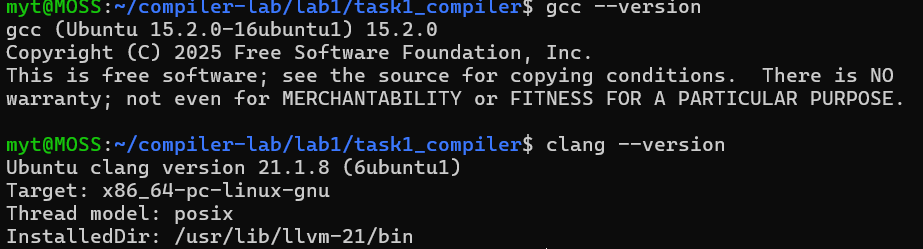
\includegraphics[width=0.82\textwidth]{task1/ma/截图2.png}}\\[0.4cm]
  \subfloat[Clang/LLVM 18.1.3（任务二）]{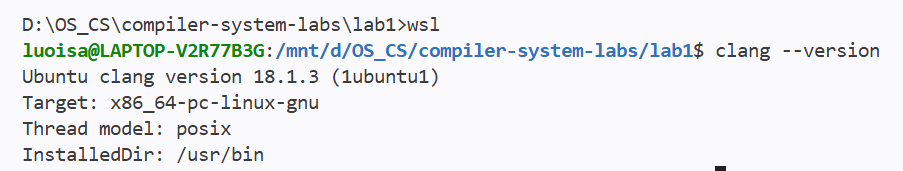
\includegraphics[width=0.82\textwidth]{task2_llvm/1.png}}\\[0.4cm]
  \subfloat[riscv64-linux-gnu-gcc 与 qemu-riscv64 版本（任务三）]{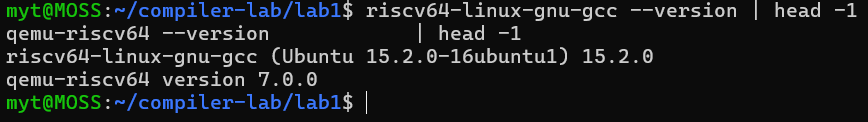
\includegraphics[width=0.82\textwidth]{task2_riscv/截图1.png}}\\[0.4cm]
\end{figure}
\begin{figure}[H]
  \centering
  \subfloat[MLIR 18.1.3（进阶要求）]{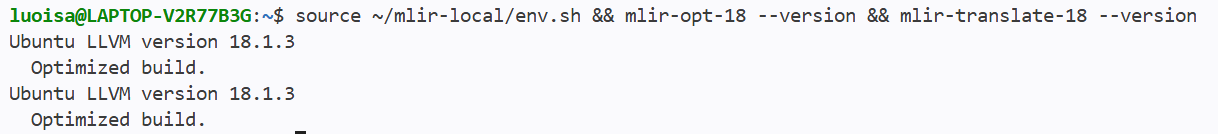
\includegraphics[width=0.82\textwidth]{advanced/1.png}}
  \caption{两位成员各任务工具链版本信息佐证}
  \label{fig:envversions}
\end{figure}

%================================================================
\section{任务一：了解你的编译器}
%================================================================

\subsection{实验原理}

\subsubsection{四个阶段的总体划分}

GCC 表面上只是一条命令，内部却把工作拆成四个依次衔接的阶段，每个阶段以上一阶段的输出作为输入：

\begin{lstlisting}
main.c --预处理--> main.i --编译--> main.s --汇编--> main.o --链接--> main
        (-E)             (-S)            (-c)            (无选项)
\end{lstlisting}

四个阶段各自的分工如表~\ref{tab:fourstage} 所示。

\begin{table}[H]
  \centering
  \small
  \setlength{\tabcolsep}{4pt}
  \begin{tabular}{>{\centering\arraybackslash}p{1.4cm}>{\centering\arraybackslash}p{2.6cm}>{\centering\arraybackslash}p{4.2cm}>{\centering\arraybackslash}p{2.2cm}>{\centering\arraybackslash}p{2.4cm}}
    \toprule
\headcol 阶段 & \headcol 执行者 & \headcol 输入 → 输出 & \headcol 产物性质 & \headcol 令流程停在此处的选项 \\
    \midrule
预处理 & 预处理器 & main.c → main.i & 文本 → 文本 & gcc -E \\
    编译 & 编译器 cc1 & main.i → main.s & 文本 → 汇编 & gcc -S \\
    汇编 & 汇编器 as & main.s → main.o & 汇编 → 二进制 & gcc -c \\
    链接 & 链接器 ld（由 collect2 封装调用） & main.o + 启动文件 + 库 → main & 二进制 → 二进制 & gcc（默认） \\
    \bottomrule
\end{tabular}
  \caption{编译过程四个阶段的划分}
  \label{tab:fourstage}
\end{table}

每完成一次转换，磁盘上都会留下一个形态不同的中间产物，正因为如此，我们才可以用 -E、-S、-c 把这条流水线在任意一步叫停、把平时被自动丢弃的中间结果保留下来逐一观察。

\subsubsection{预处理器的功能}

预处理器只在\textbf{文本层面}工作，它不理解 C 语言的语法，处理的是一行行字符，其主要职责可归纳为五类，如表~\ref{tab:cpp} 所示。

\begin{table}[H]
  \centering
  \small
  \setlength{\tabcolsep}{4pt}
  \begin{tabular}{>{\centering\arraybackslash}p{2.6cm}>{\centering\arraybackslash}p{4.6cm}>{\centering\arraybackslash}p{6cm}}
    \toprule
\headcol 功能 & \headcol 指令 & \headcol 说明 \\
    \midrule
宏定义替换 & \#define & 查询所有宏定义，用对应文本替换程序中的宏名 \\
    文件包含处理 & \#include & 把指定文件的全部内容插入到该指令所在位置，可多层嵌套 \\
    条件编译 & \#if / \#ifdef / \#else / \#elif / \#endif & 按条件决定某段代码是否参与编译 \\
    去除注释 & —— & 删除全部单行注释与多行注释 \\
    生成预处理文件 & —— & 产出 .i（C）或 .ii（C++）文件，交下一阶段使用 \\
    \bottomrule
\end{tabular}
  \caption{预处理器的五项功能}
  \label{tab:cpp}
\end{table}

\subsubsection{编译器的六个子阶段}

编译器接收预处理后的文本，输出汇编代码，这一过程被划分为六个子阶段，如表~\ref{tab:sixphase} 所示。

\begin{table}[H]
  \centering
  \small
  \setlength{\tabcolsep}{4pt}
  \begin{tabular}{>{\centering\arraybackslash}p{2.4cm}>{\centering\arraybackslash}p{2.6cm}>{\centering\arraybackslash}p{3.2cm}>{\centering\arraybackslash}p{4.6cm}}
    \toprule
\headcol 子阶段 & \headcol 输入 & \headcol 输出 & \headcol 职责 \\
    \midrule
词法分析 & 字符流 & 记号流 & 切词并标注类别 \\
    语法分析 & 记号流 & 抽象语法树 & 判断结构是否合法 \\
    语义分析 & 语法树 & 带语义信息的语法树 & 建符号表、类型检查 \\
    中间代码生成 & 语法树 & 中间表示 & 用与机器无关的形式表达 \\
    代码优化 & 中间表示 & 等价但更优的中间表示 & 提高效率、减小体积 \\
    目标代码生成 & 中间表示 & 汇编代码 & 分配存储、选择指令 \\
    \bottomrule
\end{tabular}
  \caption{编译器的六个子阶段}
  \label{tab:sixphase}
\end{table}

这六个阶段是编译原理的经典概念划分，用于描述编译器的逻辑功能。实际工具的中间表示与模型并不完全一致（GCC 内部依次为 GENERIC、GIMPLE、RTL，Clang/LLVM 则使用 LLVM IR），但每一步在概念上仍可归入上述六个阶段。

\subsubsection{汇编器的功能}

编译器产出的 main.s 仍然是\textbf{文本}，CPU 无法直接执行。汇编器（GNU 工具链中的 as）负责把这种文本形态的汇编程序翻译成\textbf{二进制目标文件}（main.o）。

汇编器与编译器的工作性质截然不同：编译器要“理解”程序的结构与含义，而汇编器只做\textbf{逐行翻译}——每一行汇编指令与一段机器码之间几乎是查表式的固定对应，汇编器既不看语法树，也不建符号的作用域，它甚至不知道这段代码究竟在做什么。

汇编器的主要职责可归纳为五类：

\begin{table}[H]
  \centering
  \small
  \setlength{\tabcolsep}{4pt}
  \begin{tabular}{>{\centering\arraybackslash}p{3cm}>{\centering\arraybackslash}p{10.2cm}}
    \toprule
\headcol 功能 & \headcol 说明 \\
    \midrule
指令编码 & 把每条汇编助记符按目标机器的指令格式翻译成二进制机器码 \\
    节（Section）组织 & 按内容性质分别放入 .text、.data、.bss、.rodata 等节 \\
    符号表构建 & 记录本文件\textbf{定义}的符号（如 main）与\textbf{引用}的外部符号（如 printf） \\
    重定位表生成 & 对地址尚不能确定的引用，留下“待填写”的记录，交链接器处理 \\
    伪指令与字面量处理 & 处理 .globl、.type、.string 等伪指令，把字符串集中在 .rodata \\
    \bottomrule
\end{tabular}
\end{table}

其中\textbf{符号表}与\textbf{重定位表}是理解后续链接过程的关键，值得单独说明。

汇编器在翻译 call printf 这条指令时，面临一个它无法解决的问题：printf 的代码位于 libc 中，此刻尚未被链接进来，它的地址根本无从得知。汇编器的做法是——先把这条指令的目标地址\textbf{填成 0}，同时在本文件的\textbf{重定位表}里登记一条记录：“在 .text 偏移这样的位置，将来需要填入 printf 的地址”。凡是跨文件、跨模块的引用（外部函数、外部变量），以及指向本文件内其他节的引用（如字符串常量所在的 .rodata），都会产生这样的“空位 + 登记”。

因此，汇编器的产物是一个“\textbf{残缺的、等待拼接的零件}”：机器码已经就绪，但凡涉及地址的地方都留了空位。正因如此，.o 文件被称为\textbf{可重定位目标文件（Relocatable Object File）}，它的 ELF 类型被标为 REL，入口地址为 0，不含任何程序头（Program Header），也就是说它根本不能被执行。

一句话概括这一阶段：\textbf{汇编器负责“翻译”，但不负责“定位”。}

\subsubsection{链接器的功能}

一个 .o 文件无法直接运行，原因有二：其一，其中的地址都是待填的“空位”；其二，它既没有程序入口 \_start，也不包含 printf 等库函数的实现。链接器（GNU 工具链中的 ld，通常由 gcc 通过 collect2 封装调用）负责把若干目标文件、启动代码与库文件拼装成一个完整的可执行文件。

链接器的工作主要有三项：

\noindent\textbf{(1)符号解析（Symbol Resolution）。} 把参与链接的全部目标文件与库视为一个整体，为每一个\textbf{未定义符号}找到唯一的\textbf{定义}。例如 main.o 中 printf、\_\_isoc99\_scanf、\_\_stack\_chk\_fail 都标记为 UND，链接器要到 libc.so.6 中把它们一一找出并绑定。若某个符号在所有输入中均无定义，就报出经典的 undefined reference to ... 错误——这条错误恰恰是符号解析过程的直接产物。

\noindent\textbf{(2)重定位（Relocation）。} 各目标文件的节区被拼装到最终虚拟地址空间之后，每个符号都有了确定的地址，链接器便\textbf{回过头把重定位表里登记的空位逐一填上}：改写目标文件中的机器码字节，并（在静态可执行文件中）删除这些已经兑现的重定位条目。

\noindent\textbf{(3)节区合并与地址分配（Section Merging \& Layout）。} 把所有输入文件的 .text 合并为最终的一个 .text，.data 合并为 .data……再依据链接脚本（linker script）规定的内存布局，为每个节区分配最终的虚拟地址，并生成\textbf{程序头（Program Header）}，描述各段在装入内存时的位置、大小与访问权限（只读/可执行/可读写）。

除这三项核心工作外，链接器还承担了若干容易被忽视的任务：

\begin{itemize}
  \item \textbf{引入启动代码。} 链接命令里会自动带上 Scrt1.o、crti.o、crtn.o 等启动文件，真正的入口 \_start 就定义在其中。\_start 并不直接调用 main，而是先调用 \_\_libc\_start\_main，由后者完成运行时初始化后，再回调我们写的 main。这就是为什么 main 既不是程序入口、也不需要自己写退出逻辑。
  \item \textbf{生成动态链接所需的 PLT 与 GOT。} 对动态库中的函数，链接器为其建立“过程链接表（PLT）”与“全局偏移表（GOT）”，使调用得以在运行时完成地址绑定。
  \item \textbf{记录运行时依赖。} 在动态段 .dynamic 中写入 NEEDED libc.so.6，并通过 INTERP 段指定动态加载器 /lib64/ld-linux-x86-64.so.2。
\end{itemize}

链接可分为两种方式，如表~\ref{tab:linktype} 所示。

\begin{table}[H]
  \centering
  \small
  \setlength{\tabcolsep}{4pt}
  \begin{tabular}{>{\centering\arraybackslash}p{1.8cm}>{\centering\arraybackslash}p{5.2cm}>{\centering\arraybackslash}p{4.4cm}>{\centering\arraybackslash}p{2cm}}
    \toprule
\headcol 方式 & \headcol 做法 & \headcol 特点 & \headcol 命令 \\
    \midrule
静态链接 & 把库函数的机器码直接复制进可执行文件 & 体积大、不依赖外部库、独立性强 & gcc -static \\
    动态链接 & 只登记“需要哪个库”，函数代码运行时才加载 & 体积小、多进程可共享、需要 PLT/GOT 支持 & gcc（默认） \\
    \bottomrule
\end{tabular}
  \caption{静态链接与动态链接}
  \label{tab:linktype}
\end{table}

动态链接之所以必须借助 PLT 与 GOT，是因为共享库在编译期无法确定加载地址（受地址空间随机化 ASLR 影响）。于是采用“\textbf{延迟绑定}”：程序中调用函数的指令并不指向函数本体，而是指向一个小小的 PLT 桩；PLT 桩再通过 GOT 表项跳转。首次调用时，GOT 表项尚指向加载器的解析代码，解析出真实地址后写回 GOT，此后调用便直接命中。这一机制将在 2.2.4 节通过反汇编直接观察到。

\subsection{实验步骤与结果}

本任务的观察对象为 task1\_compiler/src/main.c，其全部内容（14 行）如图~\ref{fig:mainc} 所示：程序读入整数 n，用 while 循环累乘得到 $n!$ 并输出，它将作为后续四个阶段全部分析的对象。

\begin{figure}[H]
  \centering
  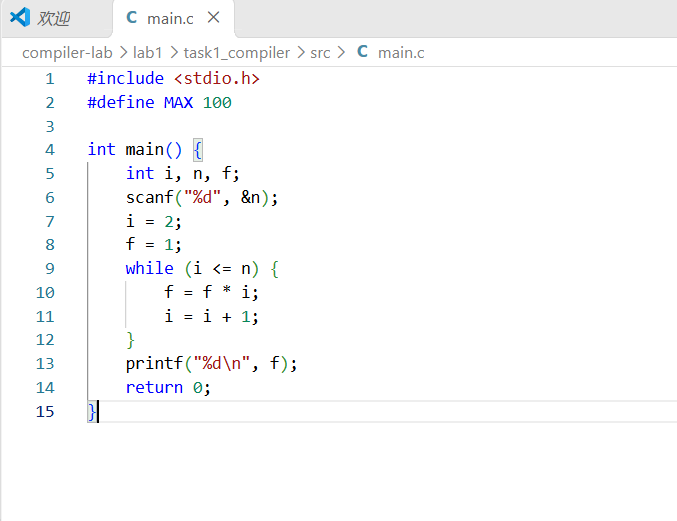
\includegraphics[width=0.72\textwidth]{task1/ma/截图1.png}
  \caption{源程序 src/main.c 的全部内容}
  \label{fig:mainc}
\end{figure}

\subsubsection{预处理阶段}

\textbf{执行命令：}

\begin{lstlisting}[language=bash]
cd ~/compiler-lab/lab1/task1_compiler
gcc src/main.c -E -o outputs/main.i
\end{lstlisting}

其中 -E 指示只进行预处理，-o 改变输出文件名。命令执行完毕，并以 ls -l outputs/ 查看，可见 main.i 已经生成，如图~\ref{fig:pre-gen} 所示。

\begin{figure}[H]
  \centering
  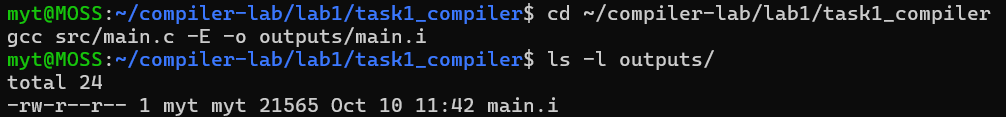
\includegraphics[width=0.85\textwidth]{task1/ma/截图3.png}
  \caption{执行预处理命令并确认 main.i 生成}
  \label{fig:pre-gen}
\end{figure}

\hfour{1、整体规模的变化}

源文件 main.c 只有 \textbf{14 行}，而预处理产物 main.i 达到 \textbf{853 行}，行数膨胀了约 60 倍。

造成这一膨胀的直接原因是第 1 行的 \#include <stdio.h>，该指令把系统头文件 stdio.h 的全部内容嵌入进来，而 stdio.h 内部又层层包含 features.h、bits/wordsize.h、sys/cdefs.h 等文件，形成一棵庞大的包含树，最终产生了远超源文件本身的文本量。\textbf{这本身就验证了预处理器“文件包含处理”的功能。}

\hfour{2、行标记（linemarker）}

main.i 第 1--20 行如图~\ref{fig:pre-linemarker} 所示，这一段 20 行之内没有出现 C 代码，全部是以 \# 开头、后接数字与文件名的结构，例如 \# 28 “/usr/include/stdio.h” 3 4，这类结构称为\textbf{行标记（linemarker）}，它不是 C 语句，而是预处理器留下的“位置记录”，用于告知后续编译器每一段文本原本来自哪个文件的第几行。

\begin{figure}[H]
  \centering
  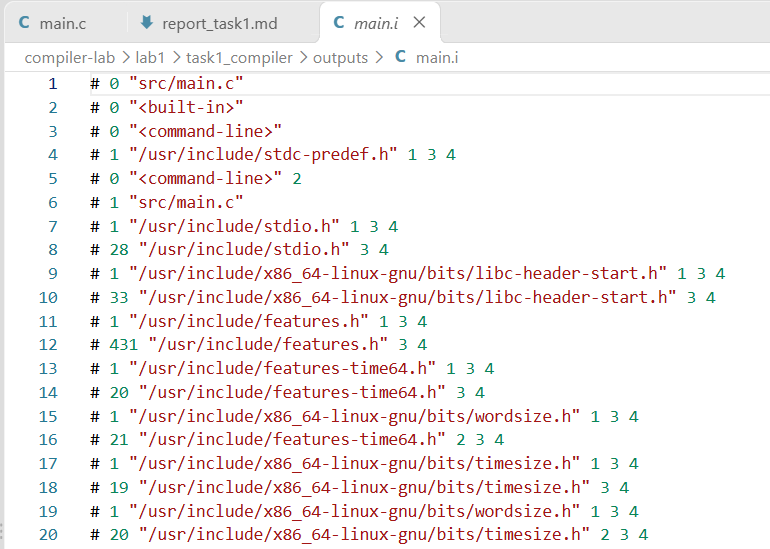
\includegraphics[width=0.8\textwidth]{task1/ma/截图4.png}
  \caption{main.i 第 1--20 行：预处理生成的行标记}
  \label{fig:pre-linemarker}
\end{figure}

其中第 1～7 行中，开头的 \# 0 "src/main.c" 表示它后面的内容归属于源文件 src/main.c；到第 7 行的 \# 1 “/usr/include/stdio.h” 1 3 4 精确标记出 \#include <stdio.h> 生效、stdio.h 内容开始被嵌入的位置；紧接着第 9、11、13 行出现的 libc-header-start.h、features.h、features-time64.h，展示了头文件“一层套一层”的展开顺序。

正是依靠这些标记，编译器在报错时才能把错误定位回用户书写的 main.c，而不是定位到展开后数百行之外的位置。整个 main.i 中共有 \textbf{117} 个行标记。

\hfour{3、真实声明的堆积}

main.i 第 45--75 行如图~\ref{fig:pre-decls} 所示。越过标记区之后，文件中开始出现真正的 C 声明。第 52 行的 typedef long unsigned int size\_t; 是全文第一句 C 代码，它来自 stddef.h；第 58 行的 typedef \_\_builtin\_va\_list \_\_gnuc\_va\_list; 来自 stdarg.h；第 72～74 行的 \_\_u\_char、\_\_u\_short、\_\_u\_int 则来自 bits/types.h。

\begin{figure}[H]
  \centering
  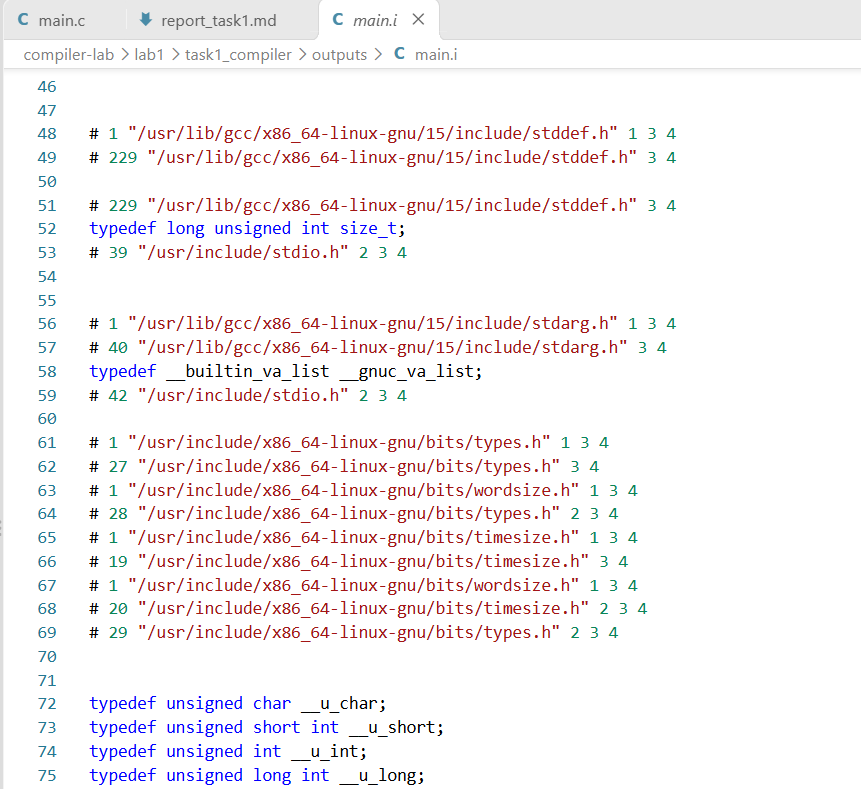
\includegraphics[width=0.8\textwidth]{task1/ma/截图5.png}
  \caption{main.i 第 45--75 行：头文件展开后堆积的真实声明}
  \label{fig:pre-decls}
\end{figure}

这些声明与源程序没有关系，都是被第 1 行的 \#include <stdio.h> 连带卷入的，段内 typedef 与行标记交替出现，恰好呈现出“进入某个头文件 → 处理其内容 → 返回上一层”的嵌套过程。

\hfour{4、宏替换与注释去除的验证}

在 main.i 中搜索 MAX，结果为空，如图~\ref{fig:pre-max} 所示。源程序中定义了 \#define MAX 100，但在预处理产物中检索 MAX，结果为 \textbf{0 处}；源程序中的注释同样为 0 处。

\begin{figure}[H]
  \centering
  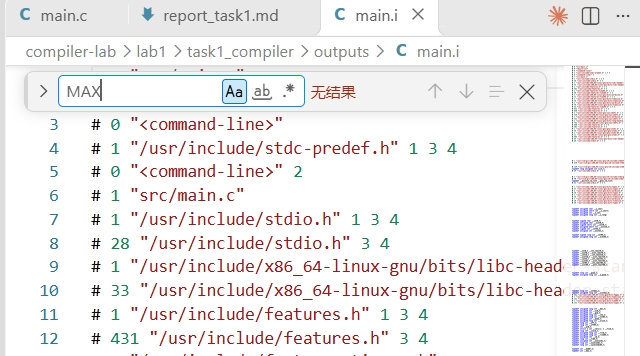
\includegraphics[width=0.65\textwidth]{task1/ma/截图6.png}
  \caption{在 main.i 中搜索 MAX，结果为空}
  \label{fig:pre-max}
\end{figure}

这一组检索验证了预处理器另外两项功能：

\begin{itemize}
  \item \textbf{宏定义替换}：宏名在预处理阶段已被替换为对应文本，\#define 指令本身也随之消失，宏只是供编译器使用的替换规则，不会作为实体保留在产物中。
  \item \textbf{去除注释}：单行注释与多行注释在预处理阶段被彻底删除，不会进入后续任何阶段。
\end{itemize}

由于 MAX 在源程序中从未被引用，替换后没有留下任何痕迹，因此在 main.i 中完全检索不到。

跳转到 main.i 第 \textbf{842} 行，即 int main() 所在位置，如图~\ref{fig:pre-main} 所示。可以看到，我们自己书写的代码被推到了文件末尾，int main() 出现在第 \textbf{842} 行，前面的 841 行全部来自头文件展开。源文件中短短 14 行的程序，预处理后变成了近八百行陌生代码之中。

\begin{figure}[H]
  \centering
  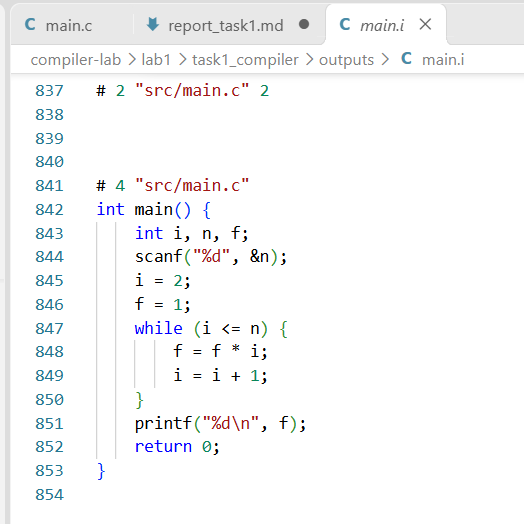
\includegraphics[width=0.65\textwidth]{task1/ma/截图7.png}
  \caption{main.i 第 842 行：int main() 位于文件末尾}
  \label{fig:pre-main}
\end{figure}

\subsubsection{编译阶段}

编译阶段的观察我们选择借助 Clang/LLVM 工具链完成，因为它提供了逐阶段导出内部表示的选项，便于对每个子阶段单独取证。

\hfour{1、词法分析}

\textbf{执行命令：}

\begin{lstlisting}[language=bash]
clang -E -Xclang -dump-tokens src/main.c
\end{lstlisting}

该命令令 Clang 在不真正编译的前提下，把源程序扫描得到的全部记号（token）打印出来，由于预处理会展开头文件，输出共有 \textbf{3042 行}，其中绝大部分来自 stdio.h。下面是位于末尾、对应我们自己所写代码的部分：

\begin{lstlisting}
int 'int'          [StartOfLine]  Loc=<src/main.c:4:1>
identifier 'main'  [LeadingSpace] Loc=<src/main.c:4:5>
l_paren '('                        Loc=<src/main.c:4:9>
r_paren ')'                        Loc=<src/main.c:4:10>
l_brace '{'        [LeadingSpace] Loc=<src/main.c:4:12>
int 'int'          [StartOfLine] [LeadingSpace] Loc=<src/main.c:5:5>
identifier 'i'     [LeadingSpace] Loc=<src/main.c:5:9>
...
identifier 'i'     [StartOfLine]  Loc=<src/main.c:7:5>
equal '='          [LeadingSpace] Loc=<src/main.c:7:7>
numeric_constant '2' [LeadingSpace] Loc=<src/main.c:7:9>
semi ';'                          Loc=<src/main.c:7:10>
...
while 'while'      [StartOfLine]  Loc=<src/main.c:9:5>
l_paren '('        [LeadingSpace] Loc=<src/main.c:9:11>
identifier 'i'                    Loc=<src/main.c:9:12>
lessequal '<='     [LeadingSpace] Loc=<src/main.c:9:14>
identifier 'n'     [LeadingSpace] Loc=<src/main.c:9:17>
r_paren ')'                       Loc=<src/main.c:9:18>
l_brace '{'        [LeadingSpace] Loc=<src/main.c:9:20>
...
string_literal '"%d\n"'           Loc=<src/main.c:13:12>
...
return 'return'    [StartOfLine]  Loc=<src/main.c:14:5>
numeric_constant '0' [LeadingSpace] Loc=<src/main.c:14:12>
semi ';'                          Loc=<src/main.c:14:13>
r_brace '}'        [StartOfLine]  Loc=<src/main.c:15:1>
eof ''                            Loc=<src/main.c:15:2>
\end{lstlisting}

上述输出中对应源程序第 4～15 行（即整个 main 函数）的部分如图~\ref{fig:lex} 所示。

\begin{figure}[H]
  \centering
  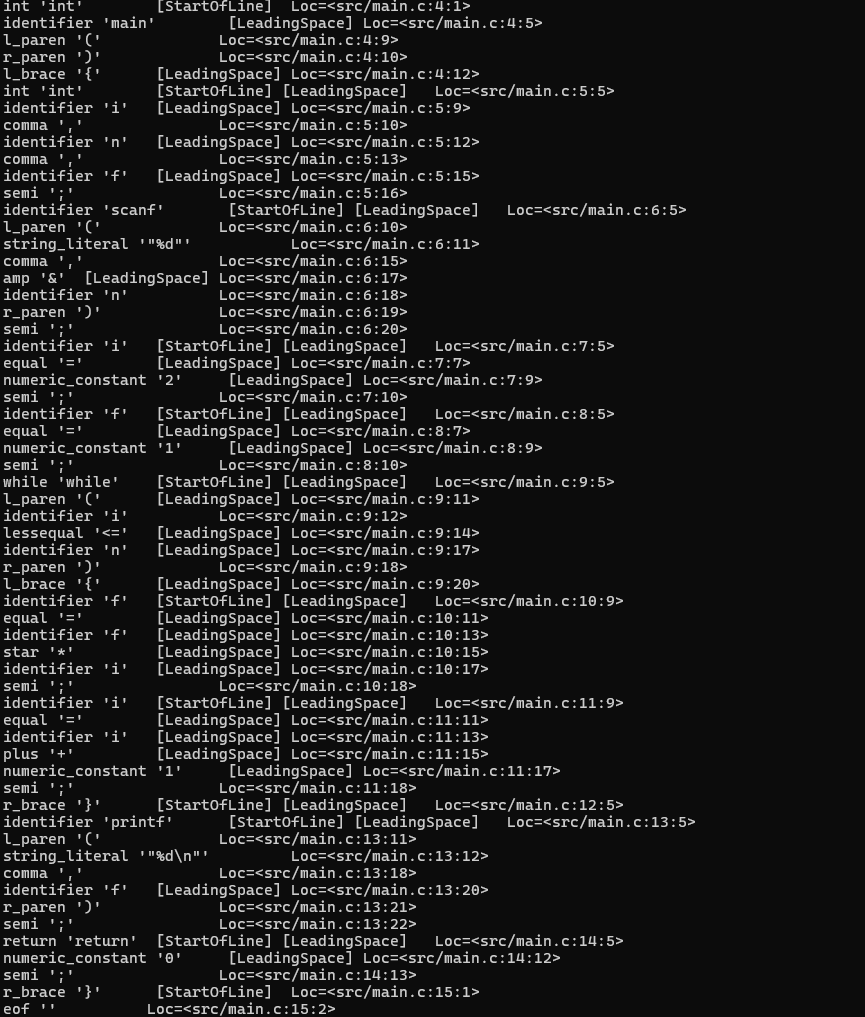
\includegraphics[width=0.8\textwidth]{task1/ma/截图8.png}
  \caption{词法分析输出中对应 main 函数的记号序列}
  \label{fig:lex}
\end{figure}

我们的结果分析如下：

（1）\textbf{源程序被扫描并切分为一个个记号，每个记号都标注了类别}。观察可知，类别包括：identifier（标识符，如 i、n、f、printf）、numeric\_constant（数值常量，如 2、1、0）、string\_literal（字符串字面量，如 “\%d\textbackslash n”）、以及 while、return 这类\textbf{关键字}，此外还有 l\_paren、r\_paren、l\_brace、r\_brace、equal、semi、lessequal、plus、star、comma、amp 等运算符与界符。可以看出，源码中出现的每个单词都被赋予了确定的类型。

（2）\textbf{记号带有位置信息}。每个记号末尾的 Loc=<src/main.c:9:14> 记录了它来自哪个文件的第几行第几列，这正是编译器能够精确定位报错位置的原因。

（3）\textbf{词法分析阶段无法判断标识符的具体含义}。i、n、f 三者都被统一标为 identifier，此时无法区分它们是变量、函数名还是别的什么；printf 同样只是一个 identifier，符号要留待语义分析阶段建立符号表后才能确定。

（4）\textbf{eof 记号表示程序结束}，最后一行 eof '' Loc=<src/main.c:15:2> 说明词法分析器已扫描到文件末尾。

至此，词法分析“将源程序转化为单词序列”的功能得到验证。

\hfour{2、语法分析}

\textbf{执行命令：}

\begin{lstlisting}[language=bash]
clang -E -Xclang -ast-dump src/main.c
\end{lstlisting}

该命令打印出 Clang 构建的\textbf{抽象语法树}。输出共 944 行，其中前 890 余行来自头文件；我们自己代码对应的 main 函数从第 895 行开始，如图~\ref{fig:ast} 所示。

\begin{figure}[H]
  \centering
  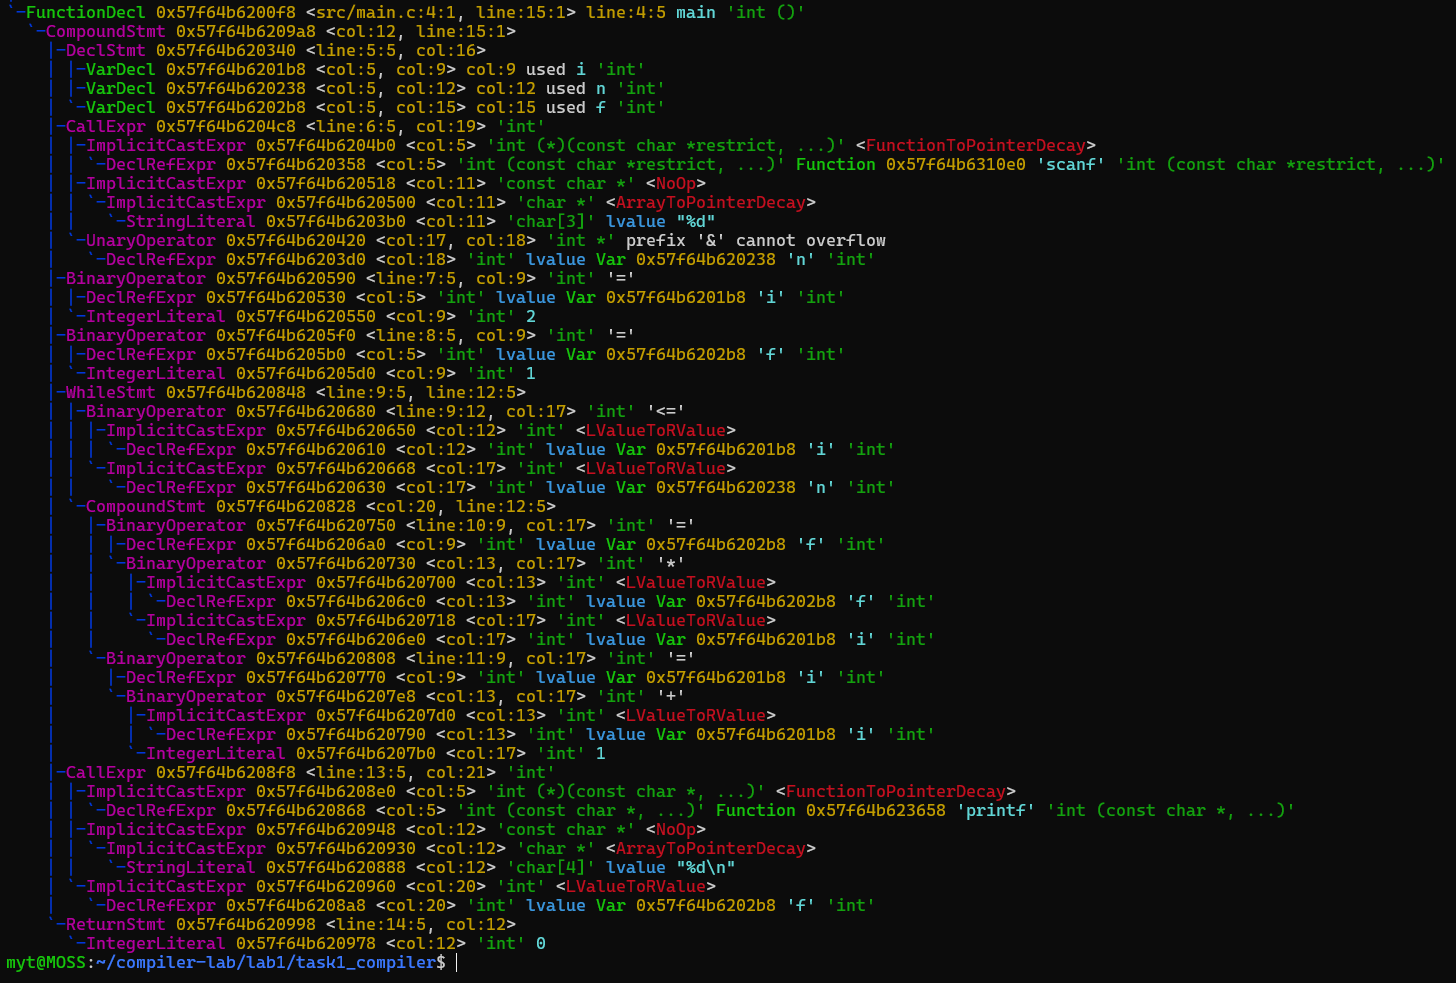
\includegraphics[width=0.78\textwidth]{task1/ma/截图9.png}
  \caption{AST 输出中 main 函数对应的部分}
  \label{fig:ast}
\end{figure}

我们的结果分析如下：

（1）\textbf{树形结构清晰地反映了源程序的语法层次}。FunctionDecl 表示函数声明，其下唯一的子结点 CompoundStmt 是函数体（复合语句）；函数体内部平级排列着：一个 DeclStmt（变量声明语句块）、两个赋值 BinaryOperator、一个 WhileStmt（循环语句）、以及函数调用 CallExpr。各结点后面的 <line:9:5, line:12:5> 说明该结点在源程序中的起止位置。

（2）\textbf{循环的语法结构被直接体现}。WhileStmt 有两个子结点：第一个是条件表达式 BinaryOperator 'int' '<='，第二个是循环体 CompoundStmt。循环体内部又包含两个赋值 BinaryOperator，其中 f = f * i 的右子树是 BinaryOperator '*'，i = i + 1 的右子树是 BinaryOperator '+'。

（3）\textbf{运算符的优先级与结合性由树的形状直接体现}。语句 f = f * i 被构造成“赋值号 = 为父结点、乘法 * 为其右子结点”，而不是 (f = f) * i，这说明优先级问题在语法分析阶段就已由文法结构解决。

（4）\textbf{语法分析只检查结构是否合法，不检查含义是否合理}。例如若把源码写成 int i = "abc";，它的结构完全符合 C 的文法，能够顺利通过语法分析，问题要到语义分析阶段才会被发现。反之，若把 while 误写成 whlie，或漏写某个分号，语法分析器就会立刻报错并指出位置——这正是语法分析“检查代码语法”的功能所在。

\hfour{3、语义分析}

语义分析在语法树的基础上，结合符号表检查源程序是否符合语言的语义定义。它主要完成类型检查、作用域解析、名称解析、控制流分析、数据流分析、符号表构建以及错误检测报告等工作。

本程序中的符号表内容如表~\ref{tab:symtab} 所示。

\begin{table}[H]
  \centering
  \small
  \setlength{\tabcolsep}{4pt}
  \begin{tabular}{>{\centering\arraybackslash}p{1.8cm}>{\centering\arraybackslash}p{3.6cm}>{\centering\arraybackslash}p{4.6cm}>{\centering\arraybackslash}p{1.8cm}}
    \toprule
\headcol 名字 & \headcol 种类 & \headcol 类型 & \headcol 作用域 \\
    \midrule
i & 变量 & int & main \\
    n & 变量 & int & main \\
    f & 变量 & int & main \\
    MAX & 宏定义（预处理后已消解） & 100 & —— \\
    scanf & 函数 & int(const char *restrict, ...) & 全局 \\
    printf & 函数 & int(const char *, ...) & 全局 \\
    \bottomrule
\end{tabular}
  \caption{main.c 中的符号表}
  \label{tab:symtab}
\end{table}

AST 中 WhileStmt 条件部分的局部放大如图~\ref{fig:while-cond} 所示。

\begin{figure}[H]
  \centering
  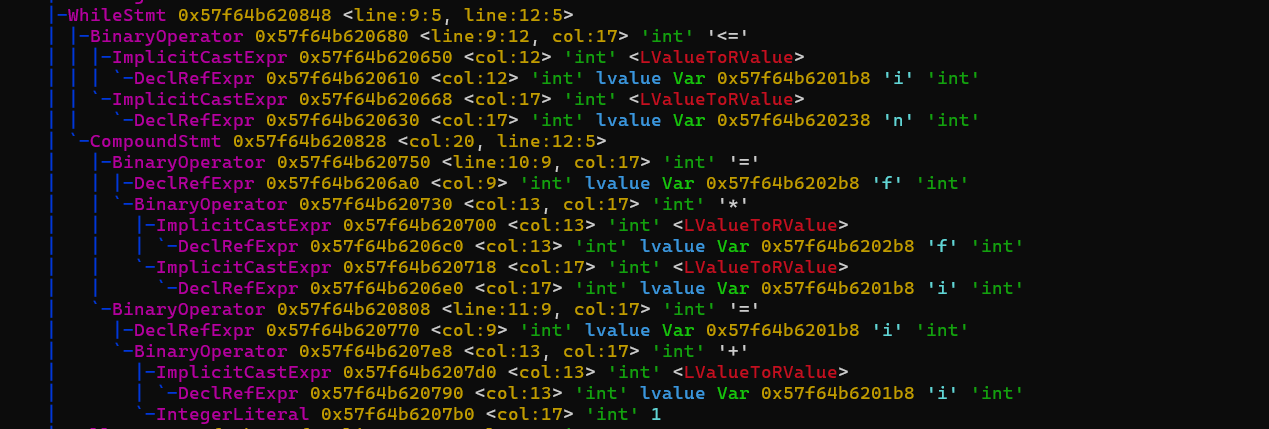
\includegraphics[width=0.85\textwidth]{task1/ma/截图10.png}
  \caption{AST 中 WhileStmt 条件部分的局部放大}
  \label{fig:while-cond}
\end{figure}

对比源码与 AST 可以发现，源码第 9 行只写了：

\begin{lstlisting}[language=C]
while (i <= n) {
\end{lstlisting}

而 AST 中对应的每个变量引用外面都被套了一层 ImplicitCastExpr <LValueToRValue>：

\begin{lstlisting}
| |-BinaryOperator <line:9:12, col:17> 'int' '<='
| | |-ImplicitCastExpr <col:12> 'int' <LValueToRValue>
| | | `-DeclRefExpr <col:12> 'int' lvalue Var 'i' 'int'
| | `-ImplicitCastExpr <col:17> 'int' <LValueToRValue>
| |   `-DeclRefExpr <col:17> 'int' lvalue Var 'n' 'int'
\end{lstlisting}

ImplicitCastExpr 表示\textbf{隐式类型转换}，<LValueToRValue> 表示“从左值取出右值”，源程序中没有书写任何转换语句，这些结点是语义分析阶段\textbf{自动插入}的——它确定了 i 和 n 都是左值，需要通过取值操作才能参与比较。

同类证据在 AST 中还有多处：
\begin{itemize}
  \item 每个 BinaryOperator 后面都标有类型 'int'。例如 BinaryOperator <line:10:9, col:17> 'int' '='，说明这个赋值运算的结果类型是 int。\textbf{这是类型检查的结果}，若两侧类型不一致，AST 上会标出相应的转换结点或直接报错。
  \item scanf 调用中，字符串字面量 “\%d” 的外面套了两层 ImplicitCastExpr：内层 <ArrayToPointerDecay>（数组退化为指针），外层 <NoOp>（仅改变类型、不产生实际代码）。源程序中写的只是 “\%d” 三个字符，编译器却知道它实际是 char[3]，需要退化成 const char * 才能作为实参。
  \item 取地址运算被标注为 UnaryOperator <col:17, col:18> 'int *' prefix '\&' cannot overflow。类型 'int *' 是语义分析推断出来的，cannot overflow 则是分析得出的额外结论。
\end{itemize}

此外，AST 中的 VarDecl ... used i 'int' 带有 used 标记，说明 i 确实被使用了；反观源码中定义的宏 MAX，由于在预处理阶段即已失去实体，语义分析阶段不会见到它，也就无法得知“定义了一个从未使用的宏”。这需要另开 -Wall 选项，由 -Wunused-macros 提示才能发现。\textbf{这印证了预处理与编译是两个彼此独立、先后衔接的过程。}

至此，语义分析阶段类型检查与符号表构建的功能得到验证。

\hfour{4、中间代码生成}

\textbf{执行命令：}

\begin{lstlisting}[language=bash]
clang -S -emit-llvm src/main.c -o outputs/main.ll
\end{lstlisting}

该命令生成 LLVM 中间表示，文件 main.ll 共 \textbf{60 行}，完整内容如图~\ref{fig:mainll} 所示，其核心部分如下：

\begin{figure}[H]
  \centering
  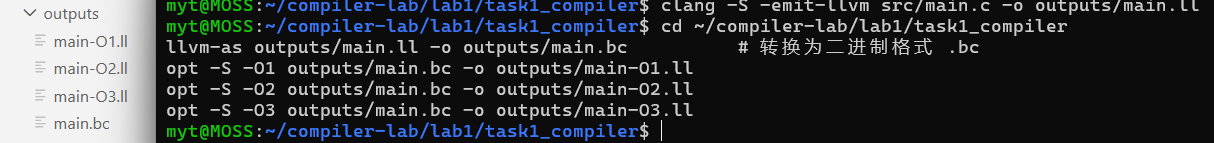
\includegraphics[width=0.78\textwidth]{task1/ma/截图11.png}
  \caption{main.ll 的完整内容}
  \label{fig:mainll}
\end{figure}

\begin{lstlisting}[language=LLVM]
; ModuleID = 'src/main.c'
source_filename = "src/main.c"
target datalayout = "e-m:e-p270:32:32-p271:32:32-..."
target triple = "x86_64-pc-linux-gnu"

@.str = private unnamed_addr constant [3 x i8] c"%d\00", align 1
@.str.1 = private unnamed_addr constant [4 x i8] c"%d\0A\00", align 1

; Function Attrs: noinline nounwind optnone uwtable
define dso_local i32 @main() #0 {
  %1 = alloca i32, align 4
  %2 = alloca i32, align 4
  %3 = alloca i32, align 4
  %4 = alloca i32, align 4
  store i32 0, ptr %1, align 4
  %5 = call i32 (ptr, ...) @__isoc99_scanf(ptr noundef @.str, ptr noundef %3)
  store i32 2, ptr %2, align 4
  store i32 1, ptr %4, align 4
  br label %6

6:                                                ; preds = %10, %0
  %7 = load i32, ptr %2, align 4
  %8 = load i32, ptr %3, align 4
  %9 = icmp sle i32 %7, %8
  br i1 %9, label %10, label %16

10:                                               ; preds = %6
  %11 = load i32, ptr %4, align 4
  %12 = load i32, ptr %2, align 4
  %13 = mul nsw i32 %11, %12
  store i32 %13, ptr %4, align 4
  %14 = load i32, ptr %2, align 4
  %15 = add nsw i32 %14, 1
  store i32 %15, ptr %2, align 4
  br label %6, !llvm.loop !6

16:                                               ; preds = %6
  %17 = load i32, ptr %4, align 4
  %18 = call i32 (ptr, ...) @printf(ptr noundef @.str.1, i32 noundef %17)
  ret i32 0
}
\end{lstlisting}

我们的结果分析如下：

（1）\textbf{文件开头给出了模块信息与目标信息}。第 1～2 行说明了模块 ID 与源文件名，第 3～4 行给出了目标数据布局（datalayout，描述各类型的对齐方式与字节序）与目标三元组（x86\_64-pc-linux-gnu，指明目标平台为 x86-64 的 Linux 系统），这说明中间代码虽然与具体机器相对解耦，但仍需记录目标平台以便后续生成代码。

（2）\textbf{两个全局变量 @.str 与 @.str.1 对应源码中的两个格式化字符串}。@.str 是 [3 x i8] c"\%d\textbackslash00"，对应 scanf 的 "\%d"；@.str.1 是 [4 x i8] c“\%d\textbackslash0A\textbackslash00”，其中 \textbackslash0A 是换行符，对应 printf 的 “\%d\textbackslash n”，源程序中的字符串常量在此被提升为全局实体。

（3）\textbf{局部变量在 LLVM 中被表示为栈上分配}。\%1 至 \%4 共四条 alloca 指令，分别对应返回值槽位、i、n、f。对照后面的 store i32 2, ptr \%2（即 i = 2）、store i32 1, ptr \%4（即 f = 1）、以及 scanf 的目标 \%3，可以确定对应关系如表~\ref{tab:varmap} 所示。

\begin{table}[H]
  \centering
  \small
  \setlength{\tabcolsep}{4pt}
  \begin{tabular}{>{\centering\arraybackslash}p{3cm}>{\centering\arraybackslash}p{8cm}}
    \toprule
\headcol 源码变量 & \headcol LLVM 中的位置 \\
    \midrule
n & \%3（scanf 读入的目标） \\
    i & \%2（被赋值为 2，并在循环中自增） \\
    f & \%4（被赋值为 1，并在循环中累乘） \\
    \bottomrule
\end{tabular}
  \caption{源码变量与 LLVM 栈位置的对应}
  \label{tab:varmap}
\end{table}

（4）\textbf{循环被表示为基本块之间的跳转}。标号 6、10、16 是三个基本块：br label \%6 进入块 6；块 6 完成条件判断，icmp sle 比较 i 与 n，br i1 \%9, label \%10, label \%16 根据结果选择跳入循环体（块 10）或跳出（块 16）；块 10 是循环体，执行乘法和自增后 br label \%6 跳回。

（5）\textbf{中间代码中出现了源码里没有的临时量与标记}。\%1～\%18 这些编号值都是编译器引入的临时名字；@\_\_isoc99\_scanf 是标准库函数的实现名；!llvm.loop !6 附在跳转指令上，是给后续优化阶段使用的循环元信息（!7 = !\{!"llvm.loop.mustprogress"\} 表示该循环必须能够推进），这些都说明中间代码是\textbf{编译器内部使用的表示}。

\hfour{5、代码优化}

代码优化是在与机器无关的层面上改进中间代码，使之运行更快、体积更小，我们用两种方式进行了观察。

\noindent\textbf{方式一：使用 opt 对已有中间代码施加优化遍。}

\begin{lstlisting}[language=bash]
cd ~/compiler-lab/lab1/task1_compiler
llvm-as outputs/main.ll -o outputs/main.bc          # 转换为二进制格式 .bc
opt -S -O1 outputs/main.bc -o outputs/main-O1.ll
opt -S -O2 outputs/main.bc -o outputs/main-O2.ll
opt -S -O3 outputs/main.bc -o outputs/main-O3.ll
\end{lstlisting}

opt 的执行过程及生成的文件如图~\ref{fig:opt} 所示。

\begin{figure}[H]
  \centering
  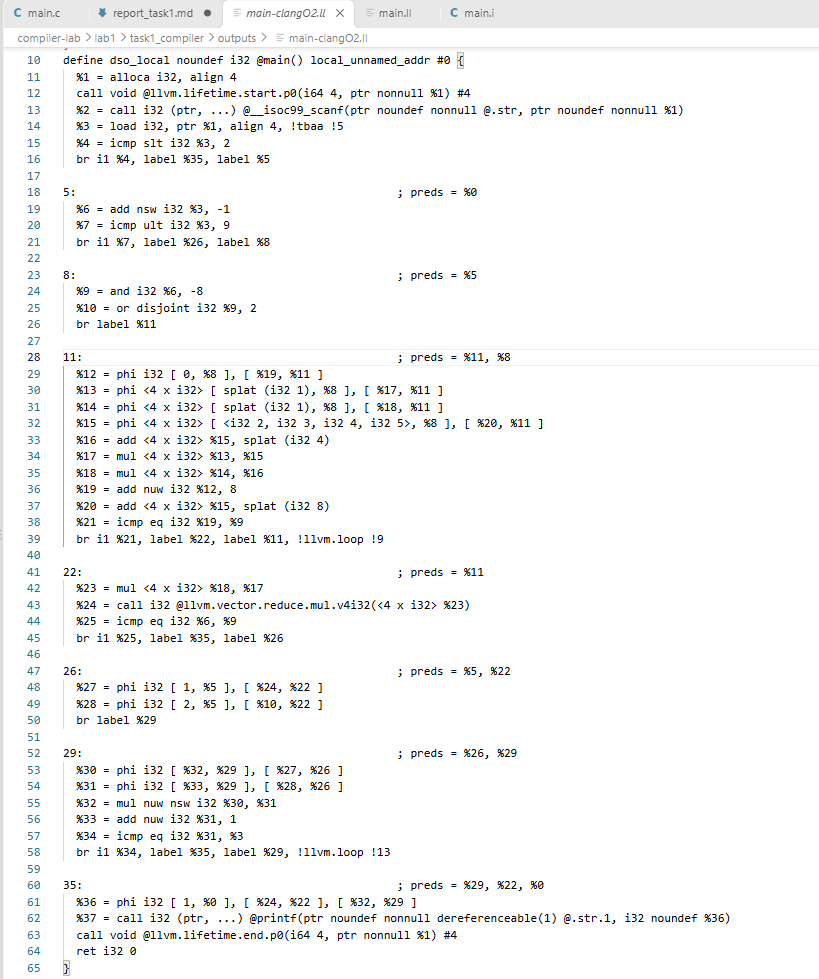
\includegraphics[width=0.85\textwidth]{task1/ma/截图12.png}
  \caption{opt 执行过程及生成的各级优化 IR 文件}
  \label{fig:opt}
\end{figure}

用 diff outputs/main.ll outputs/main-O1.ll 比较优化前后，发现差异很小，主要集中在函数与库函数声明的属性上：

\begin{itemize}
  \item \texttt{define dso\_local i32 @main() \#0 \{} 变为 \texttt{define dso\_local i32 @main() local\_unnamed\_addr \#0 \{}，新增的 local\_unnamed\_addr 表示该符号不会在链接时被外部引用，只在当前模块内可见。
  \item scanf 与 printf 的声明上新增了 captures(none)、readonly 等属性。readonly 表示函数不会修改指针所指向的内存，ncapture 表示传入的指针不会被函数保存。
  \item 属性列表中新增了 nofree、nounwind，分别表示函数不会释放内存、不会抛出异常。
\end{itemize}

但是循环部分\textbf{几乎没有变化}，原因在于 main.ll 是由 clang -S -emit-llvm 在默认（即 -O0）条件下生成的，函数带有 optnone 属性：

\begin{lstlisting}[language=LLVM]
; Function Attrs: noinline nounwind optnone uwtable
\end{lstlisting}

optnone 明确告知优化器不要对此函数做任何优化，因此 opt 只能改动函数属性，无法触及函数体。

\noindent\textbf{方式二：在生成中间代码时直接开启优化。}

\begin{lstlisting}[language=bash]
clang -O2 -S -emit-llvm src/main.c -o outputs/main-clangO2.ll
\end{lstlisting}

main-clangO2.ll 中 main 函数的完整内容如图~\ref{fig:clango2} 所示。

\begin{figure}[H]
  \centering
  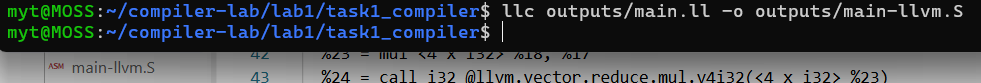
\includegraphics[width=0.78\textwidth]{task1/ma/截图13.png}
  \caption{main-clangO2.ll 中 main 函数的完整内容}
  \label{fig:clango2}
\end{figure}

优化后的 main 函数发生了三处变化：

（1）\textbf{栈上分配从 4 个减少到 1 个}。原本 \%1～\%4 四条 alloca 只剩一条，其余变量都被提升到寄存器中直接以 SSA 值的形式参与运算，不再需要内存读写。

（2）\textbf{出现了 phi 指令}。形如 \%12 = phi i32 [ 0, \%8 ], [ \%19, \%11 ] 的语句表示：从块 \%8 进入时取值为 0，从块 \%11 进入时取值为 \%19。这是\textbf{静态单赋值形式（SSA）}的标志，每个值只被赋值一次，变量的“变化”通过 phi 指令在不同控制流路径上选择取值来体现。

（3）\textbf{循环被展开并向量化}。优化后的代码使用了 <4 x i32> 类型的向量，一次处理 4 个迭代：

\begin{lstlisting}[language=LLVM]
%17 = mul <4 x i32> %13, %15
%18 = mul <4 x i32> %14, %16
...
%24 = call i32 @llvm.vector.reduce.mul.v4i32(<4 x i32> %23)
\end{lstlisting}

原程序中逐个相乘的循环，被改写为\textbf{每次完成 8 次迭代、并以 4 路 SIMD 并行计算}的形式，最后由 llvm.vector.reduce.mul 把向量中的四个乘积归约成一个结果，此外，代码中还保留了处理“不足一批的剩余迭代”的回退循环（块 \%29）。

这一对比说明同样的源代码，是否开启优化所产生的中间代码\textbf{在结构与效率上有差异}，也说明编译器的“代码优化”是决定最终程序性能的关键环节。

\hfour{6、目标代码生成}

目标代码生成以中间表示为输入，将其映射到目标机器的指令集，我们用了两种途径生成目标代码：

\begin{lstlisting}[language=bash]
# 途径一：由 LLVM 中间代码生成汇编
llc outputs/main.ll -o outputs/main-llvm.S

# 途径二：由 C 源程序经 GCC 直接生成汇编
gcc src/main.c -S -o outputs/main.s
\end{lstlisting}

llc 的执行过程及 main-llvm.S 的生成如图~\ref{fig:llc} 所示。

\begin{figure}[H]
  \centering
  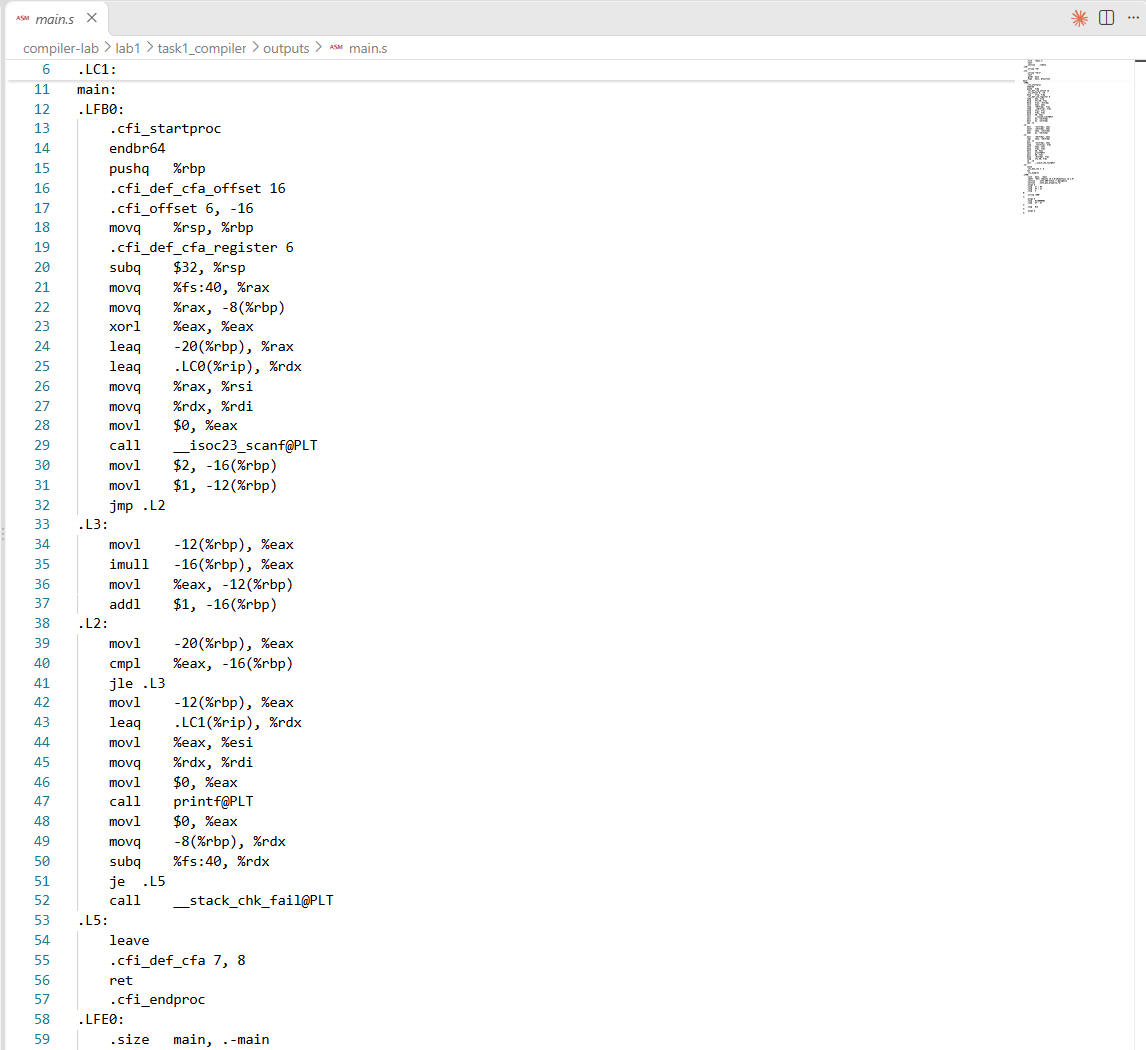
\includegraphics[width=0.85\textwidth]{task1/ma/截图14.png}
  \caption{llc 执行过程及 main-llvm.S 的生成}
  \label{fig:llc}
\end{figure}

GCC 生成的 main.s 共 \textbf{77 行}，为 AT\&T 语法的 x86-64 汇编。与 main.i 相比行数由 853 行降至 77 行，这是因为预处理产物中占据绝大部分篇幅的头文件声明，在编译阶段只用于确定类型与函数原型，本身并不产生任何指令。

该文件结构可分为三部分：开头第 4～7 行把两个字符串字面量 “\%d” 与 “\%d\textbackslash n” 集中放入 .rodata 只读数据段；第 11～59 行为 main 函数本体；其余为编译器自动附加的标识与元信息。

在 main 函数内部，源码变量与栈帧位置一一对应：n 位于 -20(\%rbp)，i 位于 -16(\%rbp)，f 位于 -12(\%rbp)。循环部分的汇编如下：

\begin{lstlisting}[language={[x86masm]Assembler}]
    movl    $2, -16(%rbp)          # i = 2
    movl    $1, -12(%rbp)          # f = 1
    jmp     .L2                        # 先跳到条件判断
.L3:                                # -- 循环体 --
    movl    -12(%rbp), %eax        #   eax = f
    imull   -16(%rbp), %eax        #   eax = eax * i
    movl    %eax, -12(%rbp)        #   f = eax
    addl    $1, -16(%rbp)          #   i = i + 1
.L2:                                # -- 条件判断 --
    movl    -20(%rbp), %eax        #   eax = n
    cmpl    %eax, -16(%rbp)        #   比较 i 与 n
    jle     .L3                        #   i <= n 则跳回循环体
\end{lstlisting}

由此可以读出目标代码生成阶段完成的三件事：

\textbf{（1）存储分配。} 三个局部变量 i、n、f 全部被分配在栈帧中，偏移分别为 -16、-20、-12。因为此处未开启优化，编译器不做寄存器分配，所有变量一律落栈，仅在需要运算时才临时调入 \%eax，这与 LLVM 中的四条 alloca 指令是同一件事的两种表示。

\textbf{（2）指令选择。} 关系运算 <= 选用 cmpl 配合 jle，乘法选用 imull，加法选用 addl。中间代码里抽象的运算，到此才落实为具体的机器指令。对照中间代码生成部分，icmp sle 对应 cmpl + jle，mul nsw 对应 imull，add nsw 对应 addl，可见两个阶段的对应关系清晰可辨。

\textbf{（3）中间表示的痕迹被消除。} LLVM 中间代码中的标号与临时值，在汇编中已换成了 .L2、.L3 这样的局部标号，\%1～\%18 这类临时值则被寄存器与栈位置取代。

此外还有两个由编译器自行决定的细节值得注意：

\textbf{循环条件的判断被安排在了循环体之后。} 源码的书写顺序是“先判断、后执行”，而在 main.s 中，标号 .L2（条件判断）位于 .L3（循环体）之后，函数入口处先用 jmp .L2 跳过去完成首次判断，此后每轮循环体执行完毕自然落入 .L2，再由 jle .L3 决定是否跳回。这说明\textbf{高级语言的程序结构与目标代码结构之间不是一一对应}，编译过程包含大量重新组织。

\textbf{部分指令与源码无关，由编译器自动插入。} 第 29 行调用的并非源码中的 scanf，而是 \_\_isoc99\_scanf@PLT；第 21～22 行与第 49～52 行出现的 \%fs:40 及 \_\_stack\_chk\_fail，则是编译器默认开启的栈保护机制，这些内容均由 GCC 自动加入，源程序中并无对应语句。

\subsubsection{汇编阶段}

\textbf{执行命令：}

\begin{lstlisting}[language=bash]
cd ~/compiler-lab/lab1/task1_compiler
as outputs/main.s -o outputs/main.o
\end{lstlisting}

as 正是 GCC 内部所使用的汇编器。执行 gcc -v 观察完整调用链时，可以清楚地看到这一步的真实命令：

\begin{lstlisting}
 as -v --64 -o /tmp/ccUkrtB5.o /tmp/ccxTwsNt.s
\end{lstlisting}

即：把编译器（cc1）产出的临时汇编文件 /tmp/ccxTwsNt.s 汇编成临时目标文件 /tmp/ccUkrtB5.o。可见前一阶段输出的 main.s，在本阶段被逐行翻译成了二进制。为展示 main.o 的生成过程，我们先将之前实验过程产生的 main.o 删除，再重新汇编生成，如图~\ref{fig:as-gen} 所示。

\begin{figure}[H]
  \centering
  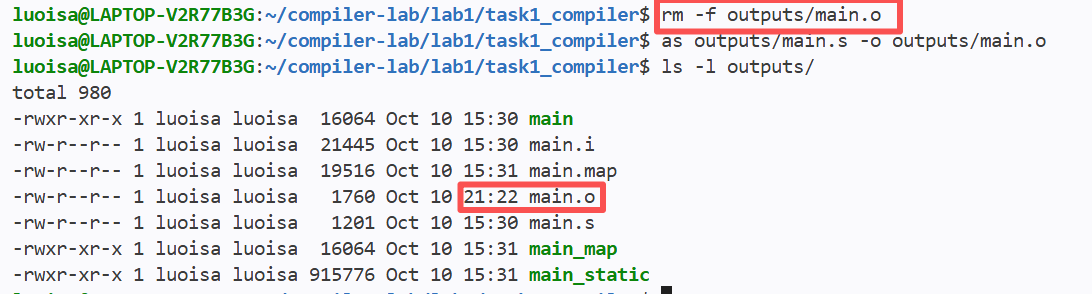
\includegraphics[width=0.85\textwidth]{task1/wu/1.png}
  \caption{删除旧产物后重新汇编生成 main.o}
  \label{fig:as-gen}
\end{figure}

\hfour{文件性质的改变}

\begin{lstlisting}[language=bash]
$ file outputs/main.o
outputs/main.o: ELF 64-bit LSB relocatable, x86-64, version 1 (SYSV), not stripped
\end{lstlisting}

输入 outputs/main.s 是\textbf{纯文本}（共 77 行），而输出 outputs/main.o 已经是\textbf{二进制}。file 输出的关键词 relocatable 表明这是一个\textbf{可重定位目标文件}，并非可执行文件。

用 readelf -h 查看其 ELF 头，可以进一步确认，输出如图~\ref{fig:readelf-ho} 所示：

\begin{figure}[H]
  \centering
  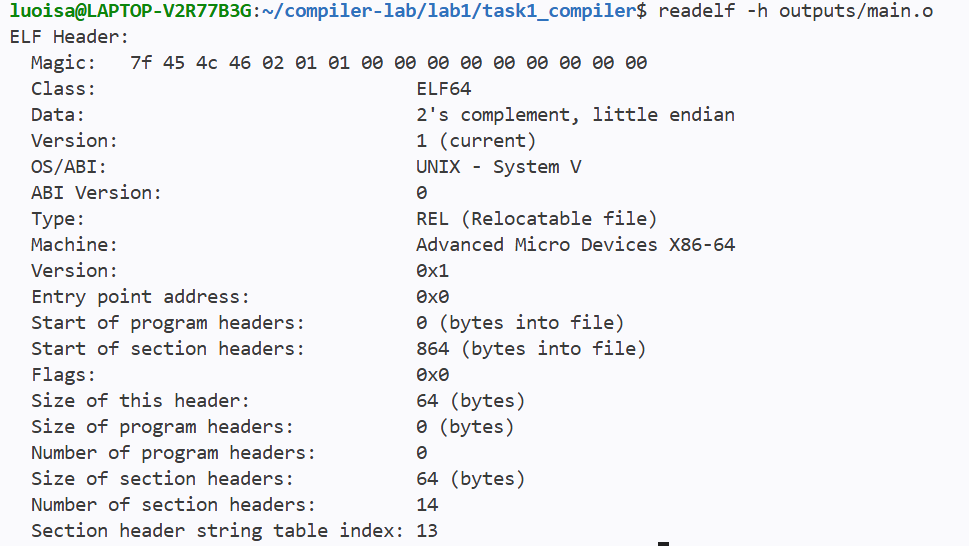
\includegraphics[width=0.8\textwidth]{task1/wu/2.png}
  \caption{readelf -h outputs/main.o 的输出}
  \label{fig:readelf-ho}
\end{figure}

\begin{lstlisting}
ELF Header:
  Class:                             ELF64
  Type:                              REL (Relocatable file)
  Machine:                           Advanced Micro Devices X86-64
  Entry point address:               0x0
  Number of program headers:         0
  Number of section headers:         14
\end{lstlisting}

三点值得注意：

\begin{itemize}
  \item \textbf{Type 是 REL。} 对照 2.2.4 节将要生成的 main（Type 为 DYN），REL 意味着这只是一个“零件”，随时可以被重新拼接、地址可以整体搬移。
  \item \textbf{Entry point address 为 0x0。} 目标文件还没有程序入口——入口 \_start 要等到链接时才由启动文件引入。
  \item \textbf{Number of program headers 为 0。} 程序头描述的是“装入内存时各段如何摆放”，而目标文件尚未确定最终地址，无从谈起装入，故一条程序头也没有。
\end{itemize}

\hfour{节区（Section）的组织}

执行 readelf -S outputs/main.o，返回结果如图~\ref{fig:readelf-s} 所示。

\begin{figure}[H]
  \centering
  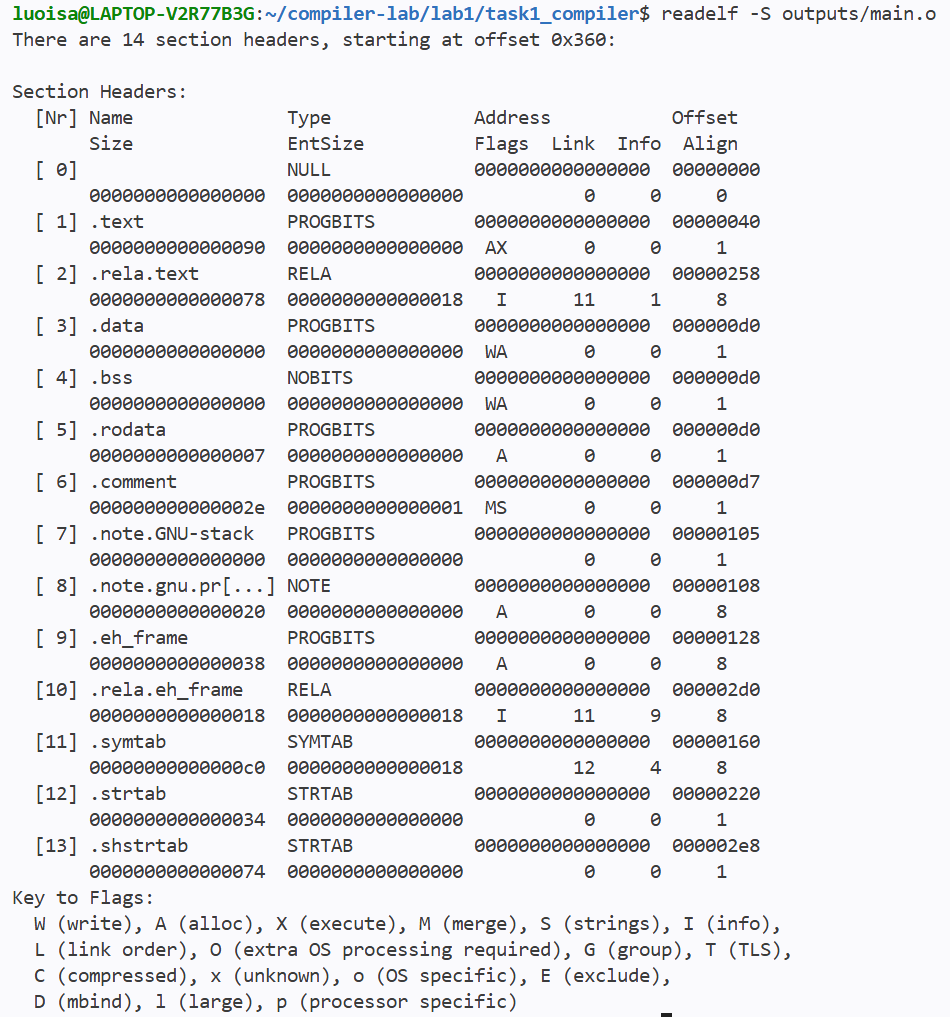
\includegraphics[width=0.85\textwidth]{task1/wu/3.png}
  \caption{readelf -S outputs/main.o：节区头表}
  \label{fig:readelf-s}
\end{figure}

整理节区头表的关键内容如下：

\begin{lstlisting}
[Nr] Name              Type             Address           Offset
  [ 1] .text             PROGBITS         0000000000000000  00000040
  [ 2] .rela.text        RELA             0000000000000000  00000258
  [ 3] .data             PROGBITS         0000000000000000  000000d0
  [ 4] .bss              NOBITS           0000000000000000  000000d0
  [ 5] .rodata           PROGBITS         0000000000000000  000000d0
  [ 6] .comment          PROGBITS         0000000000000000  000000d7
  [ 7] .note.GNU-stack   PROGBITS         0000000000000000  00000105
  [ 8] .note.gnu.pr[...] NOTE             0000000000000000  00000108
  [ 9] .eh_frame         PROGBITS         0000000000000000  00000128
  [10] .rela.eh_frame    RELA             0000000000000000  000002d0
  [11] .symtab           SYMTAB           0000000000000000  00000160
  [12] .strtab           STRTAB           0000000000000000  00000220
  [13] .shstrtab         STRTAB           0000000000000000  000002e8
\end{lstlisting}

汇编器把翻译结果按性质分门别类地放进不同的节，关键几个如表~\ref{tab:sections} 所示。

\begin{table}[H]
  \centering
  \small
  \setlength{\tabcolsep}{4pt}
  \begin{tabular}{>{\centering\arraybackslash}p{2.6cm}>{\centering\arraybackslash}p{3.4cm}>{\centering\arraybackslash}p{7.2cm}}
    \toprule
\headcol 节名 & \headcol 内容 & \headcol 在本例中的具体情况 \\
    \midrule
.text & 机器指令 & main 函数的全部指令，共 239 字节 \\
    .rodata & 只读数据 & main.s 中 .string “\%d” 与 .string “\%d\textbackslash n”（两个格式串） \\
    .data & 已初始化的可写全局/静态数据 & 本例为空（无此类变量），但汇编器仍按约定保留 \\
    .bss & 未初始化的可写数据 & 本例为空 \\
    .rela.text & .text 的重定位表 & 5 条待填记录（见本小节重定位表部分） \\
    .symtab / .strtab & 符号表与字符串表 & 记录符号名与位置（见符号表部分） \\
    \bottomrule
\end{tabular}
  \caption{main.o 中关键节区的内容}
  \label{tab:sections}
\end{table}

这里可以直接看到汇编器“节组织”与“字面量处理”两项职责：源程序里的两个字符串字面量，被汇编器依据 main.s 中的 .section .rodata 伪指令集中放进了 .rodata——因为汇编指令不能用立即数直接表示一个字符串，只能通过地址引用，故必须单独存放。此外，.data 与 .bss 虽然内容为空，却依然存在，这是为了给链接器提供统一的拼接位置。

\hfour{符号表}

执行 readelf -s outputs/main.o，返回结果如图~\ref{fig:sym-o} 所示。

\begin{figure}[H]
  \centering
  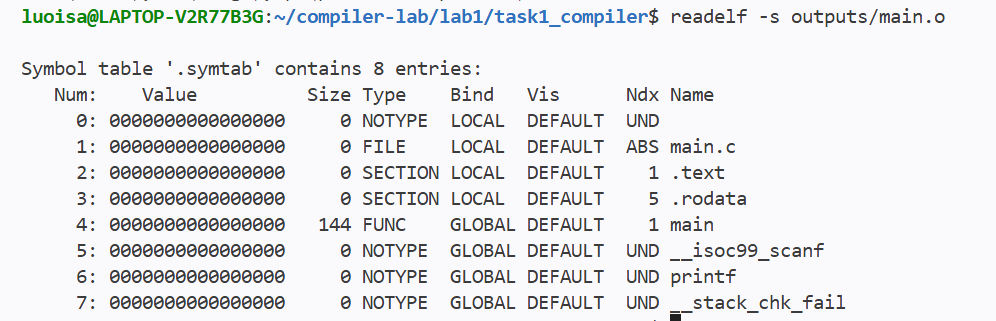
\includegraphics[width=0.85\textwidth]{task1/wu/4.png}
  \caption{readelf -s outputs/main.o：main.o 的符号表}
  \label{fig:sym-o}
\end{figure}

整理输出如下：

\begin{lstlisting}
Symbol table '.symtab' contains 8 entries:
   Num:    Value          Size Type    Bind   Vis      Ndx Name
     1: 0000000000000000     0 FILE    LOCAL  DEFAULT  ABS main.c
     2: 0000000000000000     0 SECTION LOCAL  DEFAULT    1 .text
     3: 0000000000000000     0 SECTION LOCAL  DEFAULT    5 .rodata
     4: 0000000000000000   144 FUNC    GLOBAL DEFAULT    1 main
     5: 0000000000000000     0 NOTYPE  GLOBAL DEFAULT  UND __isoc99_scanf
     6: 0000000000000000     0 NOTYPE  GLOBAL DEFAULT  UND printf
     7: 0000000000000000     0 NOTYPE  GLOBAL DEFAULT  UND __stack_chk_fail
\end{lstlisting}

符号表把符号分成两类，这正是“符号表构建”职责的体现：

\begin{itemize}
  \item \textbf{已定义的符号。} main 的 Ndx 为 1（即 .text 节），Value 为 0（在节内的偏移），Size 为 144 字节。这说明 main 已经在本文件中落地，链接器将来只需给它分配一个最终地址。
  \item \textbf{未定义的符号。} printf、\_\_isoc99\_scanf、\_\_stack\_chk\_fail 三者的 Ndx 均为 UND（undefined），Value 为 0。汇编器只知道“本文件引用了这几个名字”，既不知道它们在哪里，也不知道它们长什么样，一切留给链接器。
\end{itemize}

另外，FILE main.c 与两条 SECTION 记录是 LOCAL 的辅助符号，供调试与描述之用，不参与跨文件解析。

\hfour{重定位表}

这是本节最核心的一处证据。执行 readelf -r outputs/main.o，返回结果如图~\ref{fig:rel-o} 所示。

\begin{figure}[H]
  \centering
  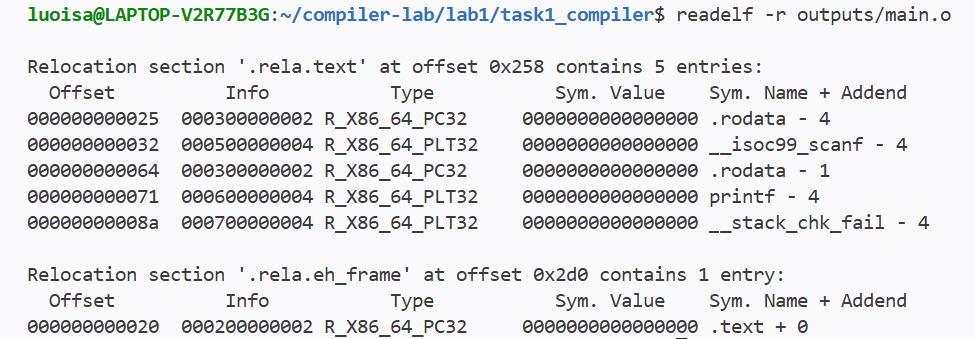
\includegraphics[width=0.85\textwidth]{task1/wu/5.png}
  \caption{readelf -r outputs/main.o：main.o 的重定位表}
  \label{fig:rel-o}
\end{figure}

这 5 条记录正是 2.1.4 节所说的“空位 + 登记”，逐条分析如下：

\begin{itemize}
  \item \textbf{Offset 指出空位在 .text 中的字节偏移。} 例如 0x32 表示 .text 第 50 字节处有一个待填的值。
  \item \textbf{两条 R\_X86\_64\_PC32（偏移 0x25、0x64）是对 .rodata 的相对寻址重定位}，对应 lea 0x0(\%rip), \%rax 之类指令中“字符串地址”被留空的部分。加数 -4（或 -1）是 x86-64 相对寻址的修正量。
  \item \textbf{三条 R\_X86\_64\_PLT32（偏移 0x32、0x71、0x8a）是对外部函数的调用重定位}，分别对应 \_\_isoc99\_scanf、printf、\_\_stack\_chk\_fail 三次调用。加数 -4 同样是相对寻址修正，它表明链接器将来要在此处填入“经由 PLT 跳转”的相对偏移。
\end{itemize}

可见汇编器对\textbf{本文件内的跨节引用}（.rodata）与\textbf{跨文件的外部引用}（printf 等）都一视同仁地留空登记——因为此刻它们都还没有确定地址。

\hfour{指令编码与“空位”的直接观察}

把 main.o 反汇编，可以看到机器码，并直接看到那些被留空的字节：

\begin{lstlisting}[language={[x86masm]Assembler}]
0000000000000000 <main>:
   0:   f3 0f 1e fa             endbr64
   4:   55                      push   %rbp
   5:   48 89 e5                mov    %rsp,%rbp
   8:   48 83 ec 20             sub    $0x20,%rsp
   c:   64 48 8b 04 25 28 00    mov    %fs:0x28,%rax
  13:   00 00
  15:   48 89 45 f8             mov    %rax,-0x8(%rbp)
  19:   31 c0                   xor    %eax,%eax
  1b:   48 8d 45 ec             lea    -0x14(%rbp),%rax
  1f:   48 89 c6                mov    %rax,%rsi
  22:   48 8d 05 00 00 00 00    lea    0x0(%rip),%rax        # 29 <main+0x29>
  29:   48 89 c7                mov    %rax,%rdi
  2c:   b8 00 00 00 00          mov    $0x0,%eax
  31:   e8 00 00 00 00          call   36 <main+0x36>
  36:   c7 45 f0 02 00 00 00    movl   $0x2,-0x10(%rbp)
  3d:   c7 45 f4 01 00 00 00    movl   $0x1,-0xc(%rbp)
  44:   eb 0e                   jmp    54 <main+0x54>
  46:   8b 45 f4                mov    -0xc(%rbp),%eax
  49:   0f af 45 f0             imul   -0x10(%rbp),%eax
  4d:   89 45 f4                mov    %eax,-0xc(%rbp)
  50:   83 45 f0 01             addl   $0x1,-0x10(%rbp)
  54:   8b 45 ec                mov    -0x14(%rbp),%eax
  57:   39 45 f0                cmp    %eax,-0x10(%rbp)
  5a:   7e ea                   jle    46 <main+0x46>
  5c:   8b 45 f4                mov    -0xc(%rbp),%eax
  5f:   89 c6                   mov    %eax,%esi
  61:   48 8d 05 00 00 00 00    lea    0x0(%rip),%rax        # 68 <main+0x68>
  68:   48 89 c7                mov    %rax,%rdi
  6b:   b8 00 00 00 00          mov    $0x0,%eax
  70:   e8 00 00 00 00          call   75 <main+0x75>
  75:   b8 00 00 00 00          mov    $0x0,%eax
  7a:   48 8b 55 f8             mov    -0x8(%rbp),%rdx
  7e:   64 48 2b 14 25 28 00    sub    %fs:0x28,%rdx
  85:   00 00
  87:   74 05                   je     8e <main+0x8e>
  89:   e8 00 00 00 00          call   8e <main+0x8e>
  8e:   c9                      leave
  8f:   c3                      ret
\end{lstlisting}

有三处观察：

\noindent\textbf{其一，每条汇编指令都被翻译成了确定的机器码。} 例如 movl \$2, -16(\%rbp)（即 i = 2）对应字节序列

\begin{lstlisting}
c7 45 f0 02 00 00 00
\end{lstlisting}

拆开看：c7 是“立即数写入内存”的操作码，45 是 ModRM 字节（表示基址寄存器 rbp、8 位位移），f0 是位移（-16 的补码），最后的 02 00 00 00 是立即数 2。\textbf{一串助记符就此固化为七字节机器码。}

\noindent\textbf{其二，call 指令的目标确实被留成了 0。} 第 31 字节处的 e8 00 00 00 00 中，e8 是 call 的操作码，其后四个字节全为 00 00 00 00——这正是汇编器留下的空位。对照重定位表，第一条涉及函数的记录 Offset = 0x32，恰好就是这条 call 指令操作码之后的第一个字节。\textbf{重定位表的用途在这里得到了最直观的印证。}

\noindent\textbf{其三，lea 0x0(\%rip), \%rax 同样留了空位。} 这条指令本意是取字符串 "\%d" 的地址，此刻填的是 0x0，对应的正是重定位表中 Offset = 0x25、指向 .rodata 的那些记录。

\subsubsection{链接阶段}

\textbf{执行命令：}

\begin{lstlisting}[language=bash]
cd ~/compiler-lab/lab1/task1_compiler
gcc outputs/main.o -o outputs/main
\end{lstlisting}

gcc 在链接时并不直接调用 ld，而是先调用 collect2 这个封装器。用 gcc -v 可以看到实际的链接命令（为便于阅读，已作换行与省略）：

\begin{lstlisting}
/usr/libexec/gcc/x86_64-linux-gnu/13/collect2 -plugin .../liblto_plugin.so ... \
  --build-id --eh-frame-hdr -m elf_x86_64 --hash-style=gnu --as-needed \
  -dynamic-linker /lib64/ld-linux-x86-64.so.2 -pie -z now -z relro \
  -o /tmp/xx \
  .../Scrt1.o .../crti.o .../crtbeginS.o \
  -L... /tmp/ccUURqiX.o -lgcc --as-needed -lgcc_s -lc ... \
  .../crtendS.o .../crtn.o
\end{lstlisting}

这条命令把本阶段的输入交代得清清楚楚，可以分为四组：

\begin{itemize}
  \item \textbf{启动文件}：Scrt1.o、crti.o、crtbeginS.o，位于目标文件之前；以及结束文件 crtendS.o、crtn.o，位于之后。入口 \_start 就在 Scrt1.o 里。
  \item \textbf{用户目标文件}：/tmp/ccUURqiX.o，即我们的 main.o。
  \item \textbf{库}：-lgcc、-lgcc\_s、-lc（即 libc）。
  \item \textbf{若干控制选项}：-pie（生成位置无关可执行文件）、-z now（立即绑定）、-z relro（重定位后只读）、--build-id（写入构建标识）。
\end{itemize}

gcc -v 输出中 collect2 的链接命令如图~\ref{fig:collect2} 所示。

\begin{figure}[H]
  \centering
  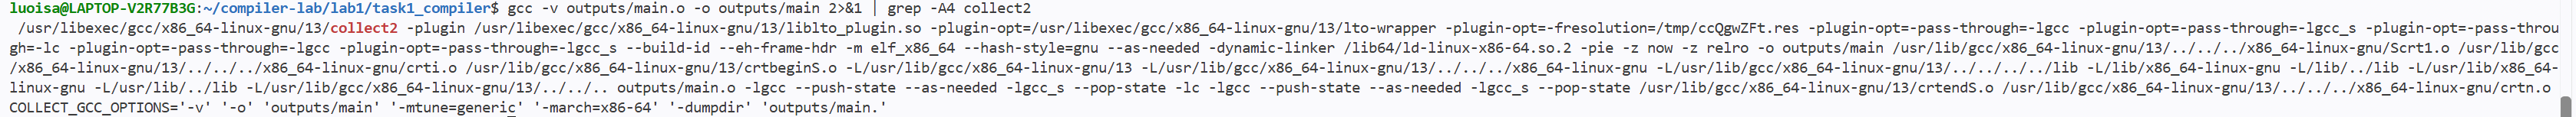
\includegraphics[width=0.9\textwidth]{task1/wu/6.png}
  \caption{gcc -v 输出中的 collect2 链接命令}
  \label{fig:collect2}
\end{figure}

\hfour{1、文件性质的改变}

\begin{lstlisting}[language=bash]
$ file outputs/main
outputs/main: ELF 64-bit LSB pie executable, x86-64, version 1 (SYSV),
  dynamically linked, interpreter /lib64/ld-linux-x86-64.so.2,
  BuildID[sha1]=c509d551b9..., for GNU/Linux 3.2.0, not stripped
\end{lstlisting}

与 main.o 相比，变化是根本性的：main.o 是 relocatable，main 是 pie executable；main.o 没有解释器，main 指定了 interpreter /lib64/ld-linux-x86-64.so.2。

再看 ELF 头：

\begin{lstlisting}
ELF Header:
  Type:                              DYN (Position-Independent Executable file)
  Entry point address:               0x10a0
  Number of program headers:         13
  Number of section headers:         31
\end{lstlisting}

file outputs/main 与 readelf -h outputs/main 的输出如图~\ref{fig:readelf-hmain} 所示。把两阶段的 ELF 头并排对照，差异一目了然，如表~\ref{tab:elfcmp} 所示。

\begin{figure}[H]
  \centering
  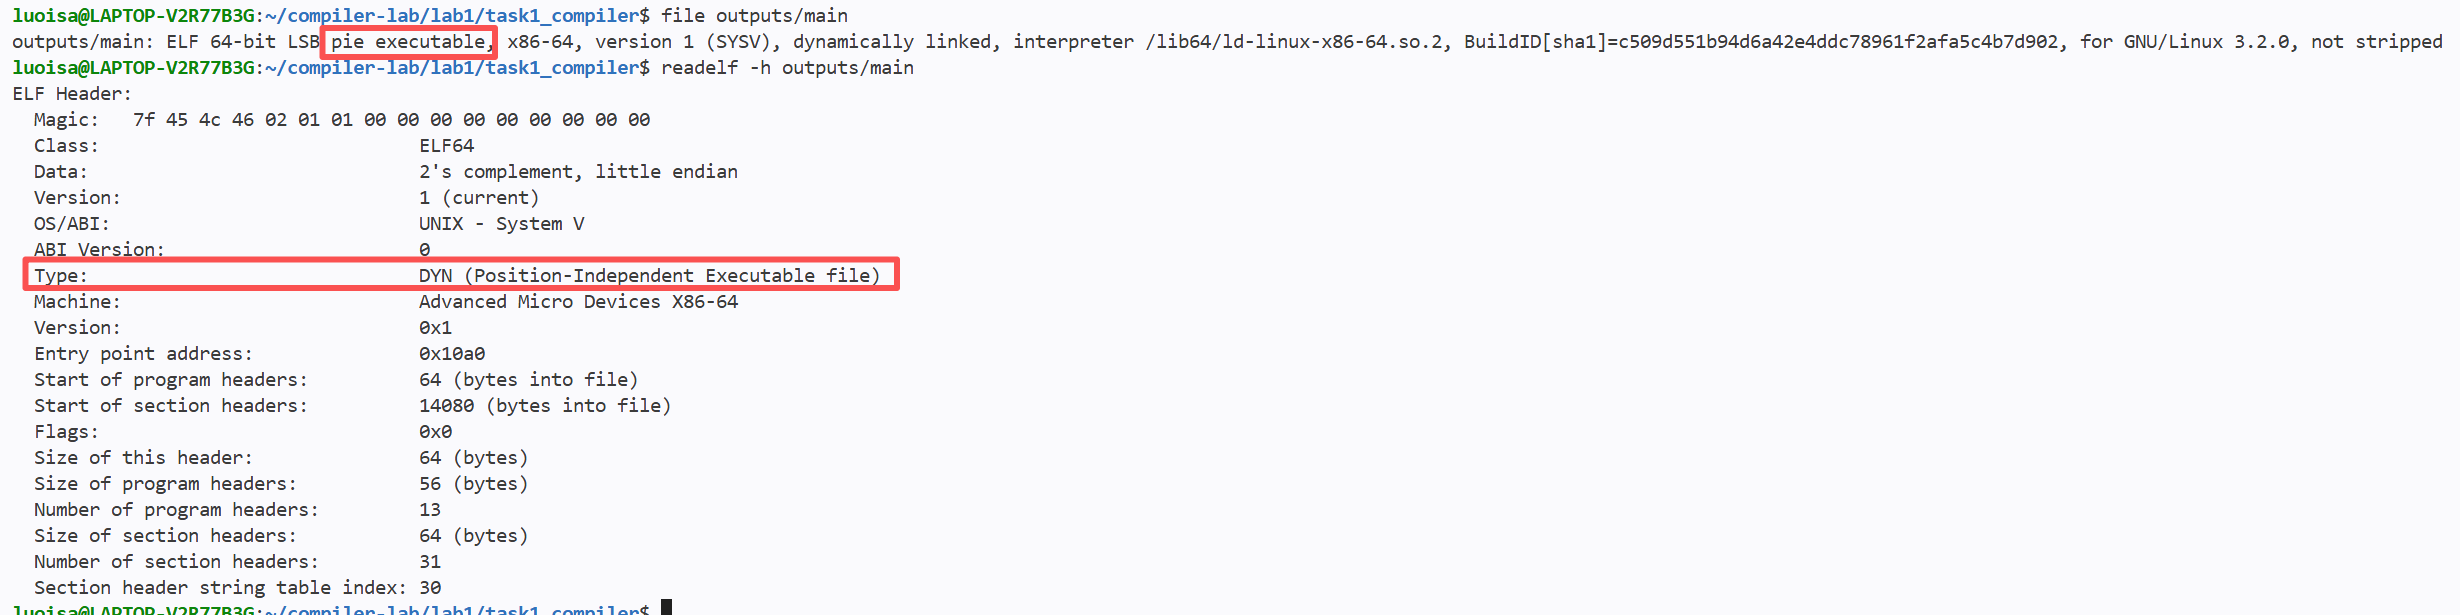
\includegraphics[width=0.92\textwidth]{task1/wu/7.png}
  \caption{file outputs/main 与 readelf -h outputs/main 的输出}
  \label{fig:readelf-hmain}
\end{figure}

\begin{table}[H]
  \centering
  \small
  \setlength{\tabcolsep}{4pt}
  \begin{tabular}{>{\centering\arraybackslash}p{3.2cm}>{\centering\arraybackslash}p{4.6cm}>{\centering\arraybackslash}p{4.6cm}}
    \toprule
\headcol 项目 & \headcol main.o（汇编产物） & \headcol main（链接产物） \\
    \midrule
类型 Type & REL（可重定位） & DYN（位置无关可执行） \\
    入口 Entry point & 0x0 & 0x10a0 \\
    程序头数量 & 0 & 13 \\
    节区数量 & 14 & 31 \\
    \bottomrule
\end{tabular}
  \caption{main.o 与 main 的 ELF 头对照}
  \label{tab:elfcmp}
\end{table}

四行数据对应了链接器四项工作的结果：类型从 REL 变为可执行；入口从“无”变为 \_start 的地址 0x10a0；程序头从 0 条增加到 13 条，用以描述装入内存的各个段；节区从 14 个增加到 31 个，因为启动文件与链接器生成的 .plt、.got、.dynamic、.init、.fini 等节被加入了进来。

\hfour{2、程序头与内存布局}

\begin{lstlisting}[language=bash]
$ readelf -l outputs/main
\end{lstlisting}

\begin{lstlisting}
Elf file type is DYN (Position-Independent Executable file)
Entry point 0x10a0
There are 13 program headers, starting at offset 64

Program Headers:
  Type           Offset   VirtAddr   FileSiz  MemSiz   Flags  Align
  PHDR           ...
  INTERP         ...      [Requesting program interpreter: /lib64/ld-linux-x86-64.so.2]
  LOAD           0x000000 0x000000   0x6e0    0x6e0    R      0x1000
  LOAD           0x001000 0x001000   0x229    0x229    R E    0x1000
  LOAD           0x002000 0x002000   0x0ec    0x0ec    R      0x1000
  LOAD           0x002da8 0x003da8   0x268    0x270    RW     0x1000
  DYNAMIC        0x002db8 0x003db8   0x1f0    0x1f0    RW     0x8
  ...
\end{lstlisting}

程序头是链接器“节区合并与地址分配”工作的直接产物：

\begin{itemize}
  \item \textbf{四个 LOAD 段}：31 个节区被按访问权限归并成 4 组，分别对应 R（只读，含 .rodata、.eh\_frame）、R E（只读可执行，即 .text、.plt）、R（只读，含 .dynsym、.dynstr 等）、RW（可读写，含 .data、.got、.bss）。注意每个 LOAD 段的 Offset 与 VirtAddr 均已按页对齐（Align 0x1000），这是装入内存所要求的。
  \item \textbf{INTERP 段}指定动态加载器 /lib64/ld-linux-x86-64.so.2，程序运行的第一步就是由内核先把它加载进来。
  \item \textbf{DYNAMIC 段}指向动态链接所需的各种表（见本小节动态链接部分）。
\end{itemize}

对比 main.o 没有任何程序头，可知“把节区组织成可装入的段”完全是链接器新增的工作。

\hfour{3、符号解析}

readelf -s outputs/main 中相关符号的输出如图~\ref{fig:sym-main} 所示。

\begin{figure}[H]
  \centering
  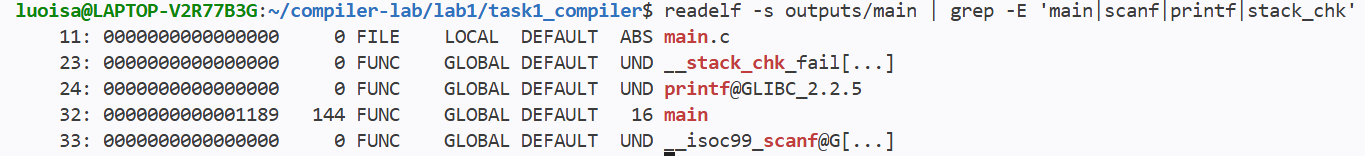
\includegraphics[width=0.85\textwidth]{task1/wu/8.png}
  \caption{readelf -s outputs/main 中相关符号的输出}
  \label{fig:sym-main}
\end{figure}

与 main.o 符号表相比，出现两处关键变化：

\noindent\textbf{其一，main 有了确定的地址。} 在 main.o 中 main 的 Value 是 0（节内偏移），而在这里变成了 0x1189——这是链接器为它分配的最终虚拟地址。\textbf{这就是“重定位”在符号层面的体现}：一旦地址确定，原先的空位就有了可填的内容。

\noindent\textbf{其二，外部符号从“裸名字”变成了“带版本号的名字”。} printf 在 main.o 中只是 printf，而在可执行文件中是 printf@GLIBC\_2.2.5；\_\_isoc99\_scanf 变成了 \_\_isoc99\_scanf@GLIBC\_2.7。这说明链接器已经在 libc.so.6 里\textbf{找到了它们的定义}，并绑定了具体的符号版本——这正是“符号解析”完成的标志。它们仍然显示为 UND，是因为其最终地址要等运行时由动态加载器写入 GOT（见本小节动态链接部分）。

\hfour{4、重定位的填补}

把“指令编码与空位”部分 main.o 的反汇编与可执行文件的反汇编对照，可以看到“空位被填上”的完整过程。可执行文件中所有对外部函数的调用都变成了经由 PLT 的调用，如图~\ref{fig:objdump-main} 所示。

\begin{figure}[H]
  \centering
  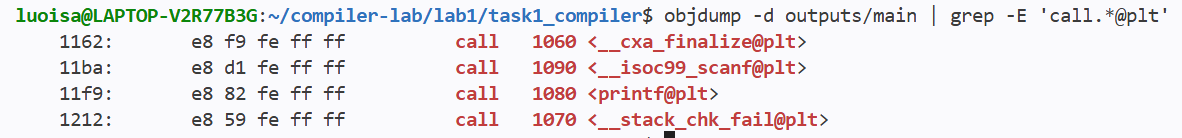
\includegraphics[width=0.9\textwidth]{task1/wu/9.png}
  \caption{objdump -d outputs/main 中 main 函数的反汇编}
  \label{fig:objdump-main}
\end{figure}

对照 main.o 中那条 31: e8 00 00 00 00 call 36 可以确认：

\begin{itemize}
  \item \textbf{原来 00 00 00 00 的位置，现在被填入了 e8 82 fe ff ff}（对应 call 1080 <printf@plt>）。原先登记在 .rela.text 中 Offset = 0x71 的那条 R\_X86\_64\_PLT32 printf 记录，就是用来填这四个字节的。
  \item call 的目标不再是函数本体，而是一个 \textbf{PLT 桩}（printf@plt 位于 0x1080）。
  \item 此外，原先 main.o 中若干涉及 .rodata 的 lea 0x0(\%rip) 空位，也都已被填入指向两个格式串的真实相对偏移。
\end{itemize}

\textbf{登记在重定位表里的 5 条记录，至此全部兑现，.rela.text 在整个可执行文件中已不复存在。}这正是链接器“重定位”职责的完整闭环。

\hfour{5、动态链接：PLT 与 GOT}

\textbf{先看运行时依赖。} 用 readelf -d 查看动态段，输出如图~\ref{fig:readelf-d} 所示。

\begin{figure}[H]
  \centering
  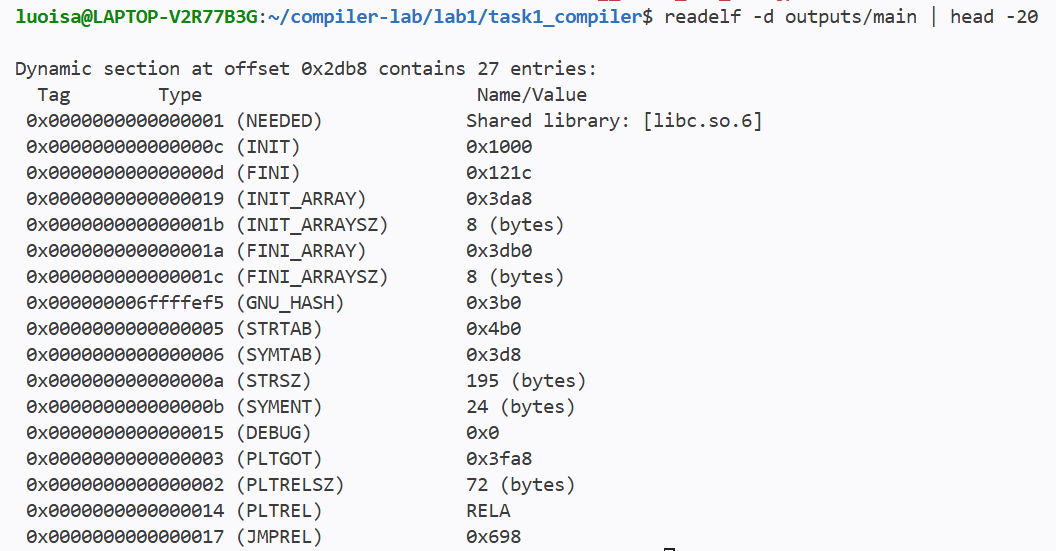
\includegraphics[width=0.8\textwidth]{task1/wu/10.png}
  \caption{readelf -d outputs/main：动态段中的运行时依赖}
  \label{fig:readelf-d}
\end{figure}

NEEDED libc.so.6 就是链接器写下的“运行时依赖”；PLTGOT、JMPREL 则指向 PLT 与 GOT 相关的表。用 ldd 可以更直观地看到运行时的库加载，如图~\ref{fig:ldd} 所示。

\begin{figure}[H]
  \centering
  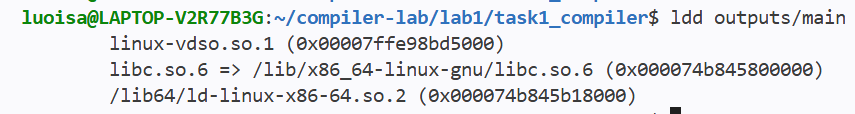
\includegraphics[width=0.8\textwidth]{task1/wu/11.png}
  \caption{ldd outputs/main：运行时动态库的加载情况}
  \label{fig:ldd}
\end{figure}

\textbf{再看 PLT 桩的结构。} 反汇编 .plt 部分，输出如图~\ref{fig:plt} 所示。

\begin{figure}[H]
  \centering
  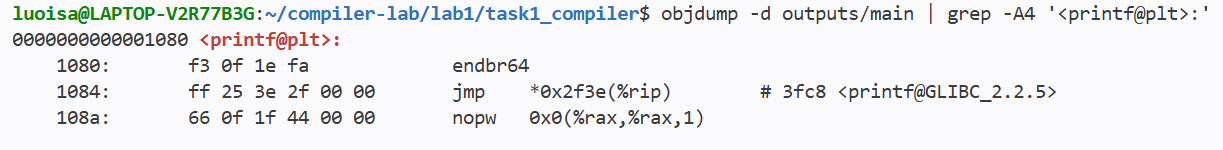
\includegraphics[width=0.85\textwidth]{task1/wu/12.png}
  \caption{.plt 节反汇编：PLT 桩的结构}
  \label{fig:plt}
\end{figure}

一个 PLT 桩只有一条有意义的指令：jmp *0x2f3e(\%rip)，即\textbf{间接跳转到一个 GOT 表项}（地址 0x3fc8）。程序调用 printf 时，实际执行的是“跳到 PLT 桩 → PLT 桩再跳到 GOT 表项所指的地址”。

\textbf{再看 GOT 表项由谁来写。} 答案在动态重定位表中（指令 readelf -r outputs/main），如图~\ref{fig:rel-main} 所示。

\begin{figure}[H]
  \centering
  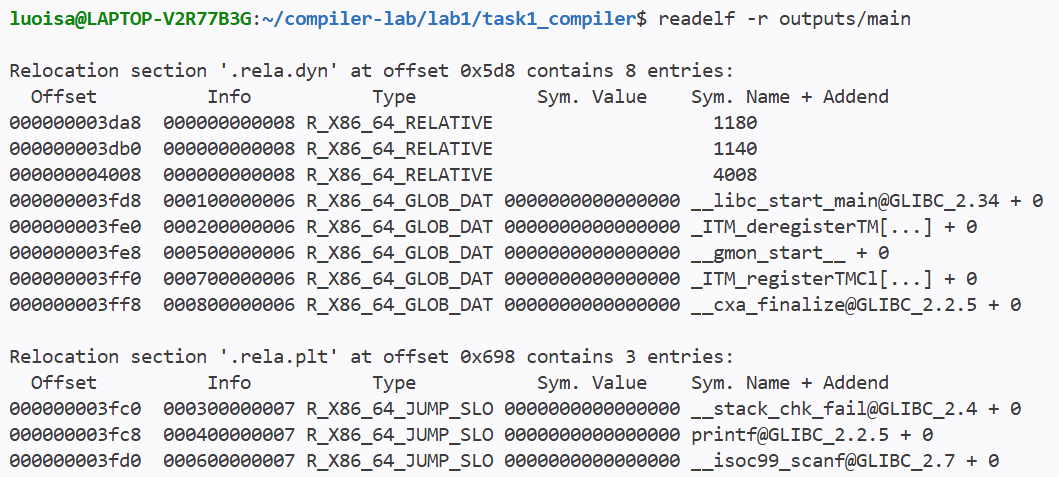
\includegraphics[width=0.85\textwidth]{task1/wu/13.png}
  \caption{readelf -r outputs/main：.rela.plt 中的动态重定位表}
  \label{fig:rel-main}
\end{figure}

.rela.plt 中的三条 R\_X86\_64\_JUMP\_SLOT 记录的 Offset 分别是 0x3fc0、0x3fc8、0x3fd0——\textbf{其中 0x3fc8 正是上面 printf@plt 所跳向的那个 GOT 表项}。这些重定位不在链接期填写，而是留给\textbf{运行时}由动态加载器补上：程序启动（或首次调用）时，加载器到 libc.so.6 中找到 printf 的真实地址，写进 0x3fc8 这个 GOT 表项，此后 jmp *0x2f3e(\%rip) 就能直达函数本体。

这一整套“\textbf{调用 → PLT 桩 → GOT 表项 → 函数本体}”的结构，就是动态链接的实现方式，也解释了为什么可执行文件里 printf 显示为 UND 却仍能正常运行——它的地址在链接期不必知道，运行时补上即可。

\hfour{6、符号解析失败的情形}

链接器的“符号解析”职责，还可以用一次\textbf{故意失败的链接}来反证。如果不把 libc 提供给链接器：

\begin{lstlisting}[language=bash]
$ ld outputs/main.o -o /tmp/t
\end{lstlisting}

输出结果如图~\ref{fig:ld-fail} 所示。

\begin{figure}[H]
  \centering
  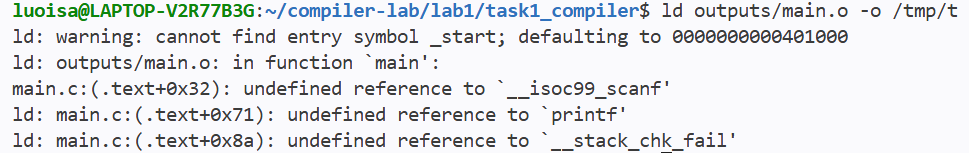
\includegraphics[width=0.85\textwidth]{task1/wu/14.png}
  \caption{直接用 ld 链接（不提供 libc）的报错}
  \label{fig:ld-fail}
\end{figure}

这条报错极有说服力：

\begin{itemize}
  \item 链接器\textbf{逐条扫描重定位表}，每遇到一个登记在案、却找不到定义的符号，就报一次 undefined reference；
  \item 报出的地址 .text+0x32、.text+0x71、.text+0x8a，与重定位表的 Offset \textbf{一字不差地吻合}。这从反面证实了重定位表的存在，也说明“符号解析”正是围绕这些登记项进行的。
  \item 此外 cannot find entry symbol \_start 则表明启动文件未被引入——正对应 2.1.5 节所说“链接器负责引入启动代码”。
\end{itemize}

\hfour{7、静态链接与动态链接的体积对比}

为验证 2.1.5 节中两种链接方式的区别，额外做一次静态链接（gcc -static outputs/main.o -o outputs/main\_static）：

\begin{lstlisting}[language=bash]
$ gcc -static outputs/main.o -o outputs/main_static
$ file outputs/main_static
outputs/main_static: ELF 64-bit LSB executable, x86-64, statically linked, ...
$ size outputs/main.o outputs/main outputs/main_static
   text    data     bss     dec     hex filename
    239       0       0     239      ef outputs/main.o
   1733     616       8    2357     935 outputs/main
 797101   23384   22472  842957   cdccd outputs/main_static
\end{lstlisting}

size 三条记录的输出，以及 file outputs/main\_static 的结果如图~\ref{fig:size} 所示。

\begin{figure}[H]
  \centering
  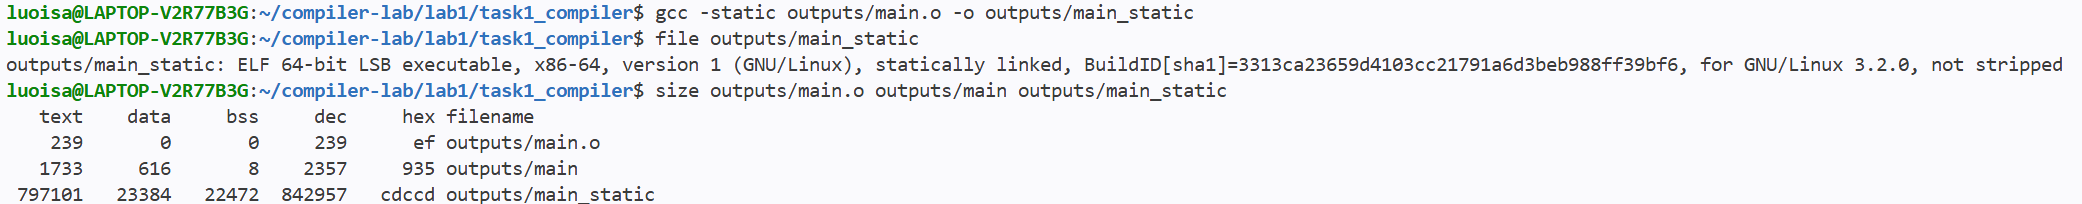
\includegraphics[width=0.85\textwidth]{task1/wu/15.png}
  \caption{三种产物的 size 对比与静态可执行文件的 file 结果}
  \label{fig:size}
\end{figure}

三个数字放在一起，链接阶段的工作量一目了然：

\begin{itemize}
  \item \textbf{main.o 的 .text 仅 239 字节}，就是 main 一个函数的机器码。
  \item \textbf{动态链接的 main 中 .text 为 1733 字节}，多出来的部分主要是启动代码（\_start）、PLT 桩以及动态链接的辅助代码——但 printf 的实现并不在其中，它仍在 libc 里。
  \item \textbf{静态链接的 main\_static 中 .text 高达 797101 字节}，因为 printf、scanf 及其依赖的整条调用链都被复制了进来。\textbf{相差约 460 倍}，这正是“静态链接把库代码复制进可执行文件”的直接后果，也解释了为什么现代系统普遍采用动态链接。
\end{itemize}

\hfour{8、运行验证}

链接产物可正常运行，如图~\ref{fig:run-main} 所示。

\begin{figure}[H]
  \centering
  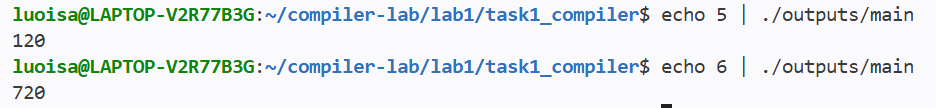
\includegraphics[width=0.75\textwidth]{task1/wu/16.png}
  \caption{运行可执行文件 main：输入 5 输出 120，输入 6 输出 720}
  \label{fig:run-main}
\end{figure}

输入 5 输出 120（$5!$），输入 6 输出 720（$6!$），与预期一致。至此，从 main.c 到可执行文件 main 的四个阶段全部走通。

\subsection{产物对比}

各阶段产物的规模与类型对比如表~\ref{tab:products} 所示。

\begin{table}[H]
  \centering
  \small
  \setlength{\tabcolsep}{4pt}
  \begin{tabular}{>{\centering\arraybackslash}p{1.8cm}>{\centering\arraybackslash}p{2.8cm}>{\centering\arraybackslash}p{2.2cm}>{\centering\arraybackslash}p{3.4cm}>{\centering\arraybackslash}p{1.8cm}>{\centering\arraybackslash}p{1.2cm}}
    \toprule
\headcol 阶段 & \headcol 命令 & \headcol 产物 & \headcol 类型 & \headcol 大小 & \headcol 行数 \\
    \midrule
（对照）源码 & —— & main.c & 文本 & 212 B & 14 \\
    预处理 & gcc -E & main.i & 文本 & 21565 B & 853 \\
    词法分析 & clang -dump-tokens & 记号流 & 文本 & —— & 3042 \\
    语法分析 & clang -ast-dump & 语法树 & 文本 & —— & 944 \\
    中间代码 & clang -emit-llvm & main.ll & 文本 & 2324 B & 60 \\
    目标代码 & gcc -S & main.s & 汇编 & 1194 B & 77 \\
    汇编 & as / gcc -c & main.o & ELF 可重定位目标文件 & 1760 B & 二进制 \\
    链接 & gcc & main & ELF 可执行文件（PIE） & 16064 B & 二进制 \\
    \bottomrule
\end{tabular}
  \caption{编译各阶段产物对比}
  \label{tab:products}
\end{table}

规模的变化并不单调：main.c 到 main.i 由 14 行猛增至 853 行，而 main.i 到 main.s 又回落至 77 行；此后 main.s 经汇编变为二进制的 main.o（1760 B），再经链接变为可执行的 main（16064 B）。\textbf{行数只在文本形态的阶段才有意义}：main.i 与 main.s 可以数行，一旦进入 main.o 与 main 这两个二进制产物，就只能用字节数来衡量了。

\subsection{小结}

\begin{enumerate}[1.]
  \item \textbf{预处理器与编译器的工作性质截然不同。} 预处理器只在文本层面操作（展开头文件、替换宏、删注释），不做语法判断；编译器则逐层完成词法、语法、语义分析，理解程序结构与含义。

  \item \textbf{各阶段产物形态逐级抽象。} 同一段 while 循环，在词法分析中是记号序列，在语法分析中是 AST 树，在中间代码中是基本块与跳转构成的控制流图，在汇编中是线性指令——描述同一件事，抽象层次逐级下降。

  \item \textbf{汇编器只翻译不定位，链接器才负责定位。} 汇编器把汇编逐行译成机器码，遇到无法确定的地址一律先填 0 并在重定位表中登记；链接器随后把这些空位逐一填上。两者分工明确：前者产出"可重定位的零件"，后者拼成"可运行的整机"。

  \item \textbf{静态链接与动态链接的体积差异显著。} 同一 main.o，动态链接后 .text 仅 1733 字节，静态链接后高达约 797101 字节，相差约 460 倍，这也解释了现代系统普遍采用动态链接及 PLT/GOT 机制的原因。
\end{enumerate}

\section{为任务二、三设计 SysY 程序}

任务二（LLVM IR 编程）与任务三（RISC-V 汇编编程）需要同一份源程序作为共同起点：前者要把它手工翻译为 LLVM IR，后者要把同一份程序手工翻译为 RISC-V 汇编。为保证两份底层代码可以相互对照、运行结果可以逐字节比对，我们在实验开始前共同设计并\textbf{冻结}了一份 SysY 示例程序 demo.c——函数签名、调用顺序与期望输出一经确定便不再改动。本章先介绍这份程序的设计思路与完整代码，归纳它所覆盖的语言特性，再给出预期运行结果与手工验算；任务二、任务三的报告中将直接引用本章，不再重复列出源码。

\subsection{demo 程序设计思路}

SysY 是编译原理课程使用的 C 语言子集，语法与 C 基本一致，但去掉了 ++、--、+= 等复合运算符，输入输出须经由课程运行库完成，我们的demo.c 在几十行篇幅内集中布置了各类语言构造，整体由三部分组成：

\begin{itemize}
  \item \textbf{两个全局对象}：只读常量 const int N = 8 作为循环上界，可写变量 int calls = 0 由递归函数累加，用于观察只读/可写两类全局量在存储与访问方式上的区别。
  \item \textbf{两个被调函数}：fib(int n) 实现递归斐波那契数列，并在每一次进入递归分支时给全局计数器 calls 加 1；calc(int a, int b) 是纯算术函数，一条表达式 (a + b) * (a - b) / b + a \% b 中同时出现加、减、乘、整除与取余五种运算。
  \item \textbf{主函数 main}：声明并初始化 5 元素整型数组 a，用第一个 while 循环做斐波那契递推并在递推过程中改写数组；输出 fib(5) 后，再用第二个带 if/else 的 while 循环按“偶数加元素、奇数加一”的规则累加数组，最后依次输出数组、累加和、calc(7,3) 的结果与递归计数 calls。
\end{itemize}

程序中的 putint、putch、putarray 均为 SysY 运行库函数，其原型在 sysy.h 中声明：putint 输出一个整数，putch 以 ASCII 码输出一个字符，putarray 先输出元素个数、再依次输出各元素。完整程序如下所示。

\begin{lstlisting}[language=C]
#include "sysy.h"

const int N = 8;
int calls = 0;

int fib(int n) {
    if (n <= 1)
        return n;
    calls = calls + 1;
    return fib(n - 1) + fib(n - 2);
}

int calc(int a, int b) {
    return (a + b) * (a - b) / b + a % b;
}

int main() {
    int a[5] = {1, 2, 3, 4, 5};
    int i = 0, x = 0, y = 1, t, sum = 0;

    while (i < N) {
        if (i < 5)
            a[i] = x;
        t = x + y;
        x = y;
        y = t;
        i = i + 1;
    }

    putint(fib(5));
    putch(10);

    i = 0;
    while (i < 5) {
        if (a[i] % 2 == 0)
            sum = sum + a[i];
        else
            sum = sum + 1;
        i = i + 1;
    }

    putarray(5, a);
    putint(sum);
    putch(10);
    putint(calc(7, 3));
    putch(10);
    putint(calls);
    putch(10);

    return 0;
}
\end{lstlisting}

\subsection{语言特性覆盖情况}

这份程序对 SysY核心特性的覆盖情况如表~\ref{tab:democover} 所示。可以看到，控制流（分支、循环）、全部整数双目运算、数组、函数调用与递归、全局常量与变量、运行库交互均有涉及，且每种特性都处在真实的数据流中，其输出结果可被独立验算，便于后续检查手写 IR 与手写汇编的正确性。

\begin{table}[H]
  \centering
  \small
  \setlength{\tabcolsep}{4pt}
  \begin{tabular}{>{\centering\arraybackslash}p{3.0cm}>{\centering\arraybackslash}p{10.5cm}}
    \toprule
\headcol 语言特性 & \headcol 程序中的体现 \\
    \midrule
顺序结构与表达式语句 & t = x + y; x = y; y = t;、calls = calls + 1; 等逐句执行的赋值 \\
    分支结构 & if (n <= 1) return n;、无 else 的 if (i < 5) a[i] = x;、带 else 的奇偶判断 if (a[i] \% 2 == 0) \dots else \dots \\
    循环结构 & 两个 while 循环：第一个 8 轮做斐波那契递推，第二个 5 轮遍历数组 \\
    算术与取余运算 & calc 的 (a + b) * (a - b) / b + a \% b 一次覆盖加、减、乘、整除、取余；另含 i + 1 等 \\
    一维数组 & int a[5] = \{1,2,3,4,5\}; 的声明与初始化、下标读 a[i] 与下标写 a[i] = x \\
    函数与递归 & fib、calc 的定义与形参，main 中的函数调用，以及 fib 对自身的递归调用 \\
    全局量 & 只读的 const int N 与可读写的 int calls，分别对应常量与变量两种全局存储 \\
    运行库交互 & 通过 putint/putch/putarray 完成整数、字符与数组输出，参数个数涵盖 1 个与 2 个 \\
    \bottomrule
\end{tabular}
  \caption{demo.c 的语言特性覆盖情况}
  \label{tab:democover}
\end{table}

\subsection{预期运行结果与手工验算}

程序没有输入，运行后向标准输出打印 5 行内容，这也是任务二手写 IR 与任务三手写汇编共同的预期输出：

\begin{lstlisting}
5
5: 0 1 1 2 3
5
14
7
\end{lstlisting}

逐行手工验算如下：

\noindent\textbf{第一行 5：} putint(fib(5)) 的输出。按斐波那契定义 $F_0=0,\ F_1=1$，$F_5=5$。

\noindent\textbf{第二行 5: 0 1 1 2 3：} putarray(5, a) 的输出。第一个循环开始时 $x=0,\ y=1$，每轮先在 $i<5$ 时把当前 $x$ 写入 a[i]，再做 $t=x+y,\ x=y,\ y=t$ 的递推。前 5 轮写入时 $x$ 依次为 $0,1,1,2,3$，故数组最终为 $\{0,1,1,2,3\}$（初值 $\{1,2,3,4,5\}$ 被全部覆盖）。

\noindent\textbf{第三行 5：} putint(sum) 的输出。第二个循环对 $\{0,1,1,2,3\}$ 按奇偶累加：偶数元素加元素本身，奇数元素加 1，即 $0+1+1+2+1=5$。

\noindent\textbf{第四行 14：} putint(calc(7, 3)) 的输出。代入得 $(7+3)\times(7-3)/3+7\bmod 3 = 10\times4/3+1 = 40/3+1 = 13+1 = 14$（整数除法向零取整）。

\noindent\textbf{第五行 7：} putint(calls) 的输出。calls 记录形参 $n>1$ 的 fib 调用次数：计算 $F_5$ 的递归树中这样的调用共有 fib(5)、fib(4) 各 1 次，fib(3) 2 次，fib(2) 3 次，合计 $1+1+2+3=7$ 次。

五行结果全部可由程序文本独立推出，因此任务二、任务三中凡手写版本的输出与上述结果逐字节相同，即可初步认定其与 SysY 源程序语义等价；两部分随后还分别用 diff 比对和交叉编译器生成版本做了进一步验证。

\section{任务二：LLVM IR 编程}

\subsection{实验原理}

\subsubsection{LLVM 的编译流程与中间表示的位置}

LLVM 采用“\textbf{前端—中间表示—后端}”的三段式结构：

\begin{lstlisting}
C 源程序
  --clang--> LLVM IR (.ll/.bc)   // 需加 -emit-llvm
  --opt--> LLVM IR (.ll/.bc)     // 优化器，可选，可多次
  --llc--> 目标汇编 (.s)          // 生成汇编
  --as--> 目标文件 (.o)           // GNU as，不是 llvm-as
  --ld--> 可执行文件              // 实际常用 clang/gcc 驱动链接
\end{lstlisting}

中间表示 LLVM IR 是这套结构的枢纽：前端只需把各种语言翻译成 LLVM IR，后端只需把 LLVM IR 翻译成各种机器的指令，前后端因此可以自由组合。本实验的对象正是这一层——\textbf{手写 LLVM IR}，就是绕开前端，直接用中间语言把程序“写”出来。

LLVM IR 有两种等价的存储形态：文本形态（.ll）是人可读的汇编式文本，可用 llvm-as 汇编为位码、用 llvm-dis 反汇编回文本；二进制形态（.bc）是机器可读的位码，由 llvm-as 生成。两者可以无损互转，本实验使用文本形态 .ll，如表~\ref{tab:llbc} 所示。

\begin{table}[H]
  \centering
  \small
  \setlength{\tabcolsep}{4pt}
  \begin{tabular}{>{\centering\arraybackslash}p{2.2cm}>{\centering\arraybackslash}p{2.0cm}>{\centering\arraybackslash}p{4.2cm}>{\centering\arraybackslash}p{5.6cm}}
    \toprule
\headcol 形态 & \headcol 扩展名 & \headcol 性质 & \headcol 工具 \\
    \midrule
文本形态 & .ll & 人可读的汇编式文本 & llvm-as 汇编为 .bc，llvm-dis 反汇编回 .ll \\
    二进制形态 & .bc & 位码，机器可读 & 由 llvm-as 生成 \\
    \bottomrule
\end{tabular}
  \caption{LLVM IR 的两种等价存储形态}
  \label{tab:llbc}
\end{table}

\subsubsection{LLVM IR 的基本结构}

一份 LLVM IR 模块（Module）自上而下包含四类内容：

\begin{enumerate}[1.]
  \item \textbf{目标信息}：target datalayout（数据布局）与 target triple（目标平台三元组）。
  \item \textbf{全局实体}：全局变量与全局常量，以 @ 开头，如 @N、@calls。
  \item \textbf{外部声明}：用 declare 声明本模块之外定义的函数，如 declare void @putint(i32)。
  \item \textbf{函数定义}：用 define 定义函数，函数体由若干\textbf{基本块（Basic Block）}组成，局部值以 \% 开头。
\end{enumerate}

其中“基本块”值得一提：它是\textbf{一段只有单一入口、以终结指令（如 br、ret）结尾的直线代码}。控制流只能在块之间通过分支指令跳转，这一约束使数据流分析变得简单，是 LLVM IR 一切优化的基础。

\subsubsection{SSA 与 PHI 节点}

LLVM IR 要求局部值满足\textbf{静态单赋值（Static Single Assignment, SSA）}形式：每个 \% 值\textbf{只能被赋值一次}。

这就带来一个问题：循环里的变量明明在反复变化，怎么用“只赋值一次”的形式表达？答案是不再让变量“变化”，而是\textbf{为每一轮迭代产生一个新值}，并在控制流汇合处用 \textbf{PHI 节点}说明“从哪条路径来，就取哪个值”：

\begin{lstlisting}[language=LLVM]
%4 = phi i32 [ %10, %3 ], [ %0, %1 ]
\end{lstlisting}

读作：若控制流从基本块 \%3 到达，\%4 取 \%10；若从 \%1 到达，则取 \%0。

需要说明的是，SSA 是“理想形式”，而 -O0 下 Clang 生成的 IR 通常并不直接采用它——局部变量一律用 alloca 在栈上开空间、再用 load/store 读写，形式上更像“内存中的变量”。栈上的内存本就可以反复改写，因而此时不需要 PHI 节点。只有在开启优化后，这些 alloca 被“提升”为寄存器中的 SSA 值，PHI 节点才随之出现。\textbf{这一点将在 4.2.5 节的两版对照中清晰可见。}

\subsubsection{SysY 语言与运行库}

SysY 是编译原理课程使用的一种 C 语言子集，语法与 C 基本一致，但去掉了 ++、--、+= 等复合运算符。SysY 程序不能直接使用标准库的输出函数，而须链接课程提供的运行库，其中常用的函数如表~\ref{tab:sylibapi} 所示。

\begin{table}[H]
  \centering
  \small
  \setlength{\tabcolsep}{4pt}
  \begin{tabular}{>{\centering\arraybackslash}p{5.2cm}>{\centering\arraybackslash}p{8.8cm}}
    \toprule
\headcol 函数 & \headcol 功能 \\
    \midrule
void putint(int a) & 输出一个整数 \\
    void putch(int a) & 输出一个字符（以其编码值） \\
    void putarray(int n, int a[]) & 输出数组：先输出个数，再依次输出各元素 \\
    int getint() & 读入一个整数 \\
    int getarray(int a[]) & 读入数组并返回个数 \\
    \bottomrule
\end{tabular}
  \caption{SysY 运行库常用接口}
  \label{tab:sylibapi}
\end{table}

本实验在 IR 中以 declare 声明这些函数，并把它们的实现放在 sylib.c 中，由链接器在链接时解析。

\subsection{实验步骤与结果}

\subsubsection{SysY 示例程序 demo.c}

本章的手写对象即第三章给出的 demo.c：任务要求针对它编写一份与 SysY 源程序等价、且能链接 SysY 运行库的 LLVM IR 程序，再使用 LLVM/Clang 与汇编器编译成目标程序，验证运行结果与源程序一致。由于第三章已对 demo.c 的源码、特性覆盖与运行结果做了详细介绍，这里不再赘述——demo.c 的运行结果就是手写 IR 程序的预期结果。

\subsubsection{SysY 运行库 sylib.c}

SysY 程序不能直接使用 C 标准库，输入输出必须经由课程提供的运行库完成。为便于在本机独立验证手写 IR，本实验编写了一份与课程运行库\textbf{接口完全一致}的 sylib.c（42 行，共 6 个函数）。

\hfour{1、函数清单与接口}

各函数的原型、功能、实现要点以及在 demo.c 中的使用情况如表~\ref{tab:sylibfull} 所示。

\begin{table}[H]
  \centering
  \small
  \setlength{\tabcolsep}{4pt}
  \begin{tabular}{>{\centering\arraybackslash}p{3.2cm}>{\centering\arraybackslash}p{2.6cm}>{\centering\arraybackslash}p{3.2cm}>{\centering\arraybackslash}p{5.0cm}}
    \toprule
\headcol 函数原型 & \headcol 功能 & \headcol 实现要点 & \headcol demo.c 是否使用 \\
    \midrule
void putint(int a) & 输出一个整数 & printf(“\%d”, a) & 输出 fib(5)、sum、calc(7,3)、calls \\
    void putch(int a) & 以编码值输出一个字符 & putchar(a) & 输出换行符 10 \\
    void putarray(int n, int a[]) & 输出数组：先输出个数，再依次输出元素 & 先 printf(“\%d:”, n)，再循环输出各元素 & 输出 a = \{0,1,1,2,3\} \\
    int getint() & 读入一个整数 & scanf(“\%d”, \&a) & 备用（本样例无输入） \\
    int getch() & 读入一个字符 & scanf(“\%d”, \&a) & 备用（本样例无输入） \\
    int getarray(int a[]) & 读入数组并返回个数 & 先读个数，再循环读入 & 备用（本样例无输入） \\
    \bottomrule
\end{tabular}
  \caption{自行编写的 sylib.c 函数清单}
  \label{tab:sylibfull}
\end{table}

\hfour{2、程序清单}

\begin{lstlisting}[language=C]
#include <stdio.h>

void putint(int a)
{
    printf("%d", a);
}

void putch(int a)
{
    putchar(a);
}

void putarray(int n, int a[])
{
    printf("%d:", n);
    for (int i = 0; i < n; i++)
        printf(" %d", a[i]);
    printf("\n");
}

int getint()
{
    int a;
    scanf("%d", &a);
    return a;
}

int getch()
{
    int a;
    scanf("%d", &a);
    return a;
}

int getarray(int a[])
{
    int n;
    scanf("%d", &n);
    for (int i = 0; i < n; i++)
        scanf("%d", &a[i]);
    return n;
}
\end{lstlisting}

\hfour{3、本运行库的三个要点}

\begin{itemize}
  \item \textbf{其一，接口必须与 demo.ll 的 declare 严格对应。} 手写 IR 中用 declare void @putint(i32)、declare void @putch(i32)、declare void @putarray(i32, ptr) 声明这些函数，链接时由本库提供实现。参数个数、类型、返回值一旦不一致，轻则类型冲突、重则链接失败；因此这份库的每个原型都是“契约”，而不是随手写的示例。
  \item \textbf{其二，它与手写 IR 处在同一编译层次。} sylib.c 由 Clang 编译成目标代码，demo.ll 经 llvm-as / clang 编译成目标代码，二者\textbf{分别编译、一起链接}。也就是说，\textbf{手写的中间代码与编译器产出的中间代码是平级的}，最终都化为机器码参与链接——这正是“中间表示作为前后端枢纽”的意义所在。
  \item \textbf{其三，输入类函数在本样例中为备用。} demo.c 只做输出，故 getint/getch/getarray 并未被调用；提供它们是为了让这份运行库与课程接口完全对齐，便于日后扩展带输入的样例程序。getch 之所以也读整数，是为了与 SysY 运行库“以 int 承载字符编码”的约定保持一致。
\end{itemize}

\subsubsection{手写 LLVM IR：demo.ll}

最终写出的 demo.ll 共 209 行，下面对代码逐块分析（完整代码见 GitHub 仓库 code/task2\_llvm/demo.ll）。

\hfour{1、模块头与目标平台}

\begin{lstlisting}[language=LLVM]
target triple = "x86_64-pc-linux-gnu"
\end{lstlisting}

target triple 声明这份 IR 面向的目标平台，三段分别是“架构-厂商-操作系统”：x86\_64 是 64 位 x86 架构；pc 是通用 PC 的厂商字段（本机 clang --version 显示的默认 Target 即 x86\_64-pc-linux-gnu，也可用 clang -print-target-triple 直接查到）；linux-gnu 是 GNU/Linux。它的作用有三点：\textbf{其一}，决定指针宽度（本平台为 64 位，因此 GEP 索引要用 i64）；\textbf{其二}，决定调用约定与栈帧布局；\textbf{其三}，指导后端选择指令集。

与 Clang 自动生成的 IR 相比，这里省略了 target datalayout 一行——Clang 会显式列出各类型对齐、字节序等布局细节，手写时由 triple 推断即可。

\hfour{2、全局变量与常量}

\begin{lstlisting}[language=LLVM]
@N = constant i32 8          ; const int N = 8
@calls = global i32 0        ; int calls = 0
\end{lstlisting}

这两行对应源程序里的 const int N = 8; 与 int calls = 0;：

\begin{itemize}
  \item \textbf{命名规则}：全局标识符以 @ 开头（局部的寄存器/变量以 \% 开头）。@N、@calls 就是符号名，链接后会被写入符号表。
  \item \textbf{constant 与 global 的区别}：@N 用 constant 修饰，表示\textbf{只读}，任何向它 store 的行为都是非法的（对应 C 的 const）；@calls 用 global，表示\textbf{可读写}——fib 中要修改它，所以必须是 global。
  \item \textbf{类型与初值必须写全}：LLVM IR 是强类型的，定义全局量时要同时给出类型（i32）与初值（8/0），不能像 C 那样只声明不给初值。手写时可省略 align，而 Clang 自动生成的 IR 会补上 align 4。
  \item \textbf{在函数中访问全局量}：@calls 这个名字本身就是“指针常量”（指向该全局量的地址），所以 load i32, ptr @calls, align 4 即可取值，store i32 \%inc, ptr @calls, align 4 即可写入。这与局部变量用 alloca 得到的指针在用法上完全一致。
\end{itemize}

\hfour{3、外部函数声明：SysY 运行库接口}

\begin{lstlisting}[language=LLVM]
declare void @putint(i32)
declare void @putch(i32)
declare void @putarray(i32, ptr)
\end{lstlisting}

declare 表示\textbf{只声明、不定义}：告诉编译器“这几个符号在别处实现”，从而允许本模块调用它们，函数体由 sylib.c 提供，最终在链接阶段接上。三条声明的要点：

\begin{itemize}
  \item \textbf{返回类型}：三者都返回 void，因为运行库函数没有返回值。
  \item \textbf{参数类型}：putint/putch 接收一个 i32；putarray 接收 i32（元素个数）与 ptr（首元素地址）。注意第二个参数用的是不透明指针 ptr，而不是 [5 x i32]*——运行库只关心“一个指向 int 的指针”，数组长度由第一个参数单独告知。
  \item \textbf{调用形式}：调用时须写明返回类型与实参类型，如 call void @putint(i32 \%call)；有返回值的则是 \%call12 = call i32 @calc(i32 7, i32 3)。
  \item \textbf{一致性要求}：这些声明必须与 sylib.c 中 C 函数的原型严格对应，否则会引发类型不匹配或链接错误。
\end{itemize}

\hfour{4、变量的表示与初始化}

LLVM IR 里\textbf{没有“局部变量声明”这一语法}。在 -O0 风格下，每个局部变量都对应一条 alloca（在栈上分配一块空间），之后的读、写分别用 load、store 完成。以 main 为例：

\begin{lstlisting}[language=LLVM]
entry:
  %retval = alloca i32, align 4
  %a = alloca [5 x i32], align 4
  %i = alloca i32, align 4
  %x = alloca i32, align 4
  %y = alloca i32, align 4
  %t = alloca i32, align 4
  %sum = alloca i32, align 4
  store i32 0, ptr %retval, align 4
\end{lstlisting}

\begin{itemize}
  \item 每条 alloca 的含义是“在栈上开辟 4 字节、按 4 字节对齐”；\%a 的类型是 [5 x i32]，即“5 个 i32 组成的数组”，因此一次分配 20 字节。
  \item \textbf{标量的初始化}就是一次 store，例如 store i32 0, ptr \%i, align 4 对应 int i = 0;；未显式赋初值的变量（如 t）无需 store。
  \item \textbf{数组的初始化没有专用指令}，只能逐元素“取地址、再存储”。int a[5] = \{1,2,3,4,5\}; 被写成 5 组 getelementptr + store：
\end{itemize}

\begin{lstlisting}[language=LLVM]
  ; int a[5] = {1, 2, 3, 4, 5};
  %a.0 = getelementptr inbounds [5 x i32], ptr %a, i64 0, i64 0
  store i32 1, ptr %a.0, align 4
  %a.1 = getelementptr inbounds [5 x i32], ptr %a, i64 0, i64 1
  store i32 2, ptr %a.1, align 4
  ... （其余三个元素同理）
\end{lstlisting}

这正是 Clang 在 -O0 下的写法之一；而到 -O2，编译器会改用 memcpy 甚至一条向量 store <4 x i32> 把多个元素一次性写入（见 4.2.5 节），差别非常直观。

\textbf{为什么连函数参数也要 alloca？} 因为 LLVM IR 的参数在本函数内是\textbf{不可重新赋值的 SSA 值}。若某个参数需要像变量一样被改写，就必须先 store 到栈空间，此后通过 load/store 读写——这就是 fib、calc 里每个参数都有一条 \%x.addr = alloca 的原因。

\hfour{5、函数 fib：条件分支与递归}

fib 是递归函数，集中体现了\textbf{条件分支的拆解}与\textbf{含函数调用时的访存行为}。

\begin{lstlisting}[language=LLVM]
define i32 @fib(i32 %n) {
entry:
  %n.addr = alloca i32, align 4
  store i32 %n, ptr %n.addr, align 4
  %0 = load i32, ptr %n.addr, align 4
  %cmp = icmp sle i32 %0, 1
  br i1 %cmp, label %if.then, label %if.end

if.then:
  %1 = load i32, ptr %n.addr, align 4
  ret i32 %1

if.end:
  %2 = load i32, ptr @calls, align 4
  %inc = add nsw i32 %2, 1
  store i32 %inc, ptr @calls, align 4
  %3 = load i32, ptr %n.addr, align 4
  %sub1 = sub nsw i32 %3, 1
  %call1 = call i32 @fib(i32 %sub1)
  %4 = load i32, ptr %n.addr, align 4
  %sub2 = sub nsw i32 %4, 2
  %call2 = call i32 @fib(i32 %sub2)
  %add = add nsw i32 %call1, %call2
  ret i32 %add
}
\end{lstlisting}

逐项说明：

\begin{itemize}
  \item \textbf{函数签名 define i32 @fib(i32 \%n)}：返回 i32，接收一个 i32 参数 \%n。与 C 不同，LLVM IR 的参数在本函数内是\textbf{不可重新赋值}的 SSA 值，若要像局部变量那样改写它，需要先把值 store 到一块栈空间里。
  \item \textbf{\%n.addr = alloca 与 store}：在栈上分配 4 字节、按 4 字节对齐，并把参数 \%n 写进去。此后对 n 的每次读取都变成一次 load。这份“多余的复制”在 -O0 下必然存在，正是优化器后来要消除的对象（见 4.2.5 节）。
  \item \textbf{icmp sle}：有符号的“小于等于”比较（signed less or equal），结果为 i1 类型（一位布尔值）。C 的关系与逻辑运算在 LLVM IR 中的对应如表~\ref{tab:icmp} 所示。
\end{itemize}

\begin{table}[H]
  \centering
  \small
  \setlength{\tabcolsep}{4pt}
  \begin{tabular}{>{\centering\arraybackslash}p{3.2cm}>{\centering\arraybackslash}p{4.2cm}>{\centering\arraybackslash}p{6.6cm}}
    \toprule
\headcol C 运算符 & \headcol LLVM IR & \headcol 说明 \\
    \midrule
a <= b & icmp sle & signed less or equal \\
    a < b & icmp slt & signed less than \\
    a == b & icmp eq & equal \\
    a != b & icmp ne & not equal \\
    a \&\& b & and i1 & 仅在两边都已求出的前提下 \\
    !a & xor i1 a, true & 布尔值取反 \\
    \bottomrule
\end{tabular}
  \caption{C 关系/逻辑运算到 LLVM IR 的对应}
  \label{tab:icmp}
\end{table}

\begin{itemize}
  \item \textbf{br i1 \%cmp, label \%if.then, label \%if.end}：条件分支，是基本块的\textbf{终结指令}。C 的 if 在此被彻底拆解为“比较 + 条件跳转”，if 这个关键字不再存在。
  \item \textbf{if.then 与 if.end 两个基本块}：分别对应 n <= 1 与 n > 1 两条路径，二者都以 ret 结束，没有合流点——因此\textbf{不需要 PHI 节点}。
  \item \textbf{add nsw / sub nsw}：nsw 是“No Signed Wrap”的缩写，告诉优化器“假定运算不产生有符号溢出”。这一许诺使优化器可以放心地做代数化简（例如把 a + 1 - 1 直接化简为 a）。若程序确实依赖溢出行为，就不该加 nsw。
  \item \textbf{递归调用 call i32 @fib(i32 \%sub1)}：fib(n-1) 与 fib(n-2) 两次调用分别产生 \%call1、\%call2，再相加返回。\textbf{值得注意的是，每次进入 if.end 之前都要重新 load 一次 \%n.addr}——因为中间夹着函数调用，优化器在 -O0 下不敢假定内存未被改动。
\end{itemize}

\hfour{6、函数 calc：算术运算与运算符映射}

calc 是纯算术函数，用它来展示 LLVM IR 的算术指令与 C 运算符的一一对应。

\begin{lstlisting}[language=LLVM]
define i32 @calc(i32 %a, i32 %b) {
entry:
  %a.addr = alloca i32, align 4
  %b.addr = alloca i32, align 4
  store i32 %a, ptr %a.addr, align 4
  store i32 %b, ptr %b.addr, align 4
  %0 = load i32, ptr %a.addr, align 4
  %1 = load i32, ptr %b.addr, align 4
  %add = add nsw i32 %0, %1
  %2 = load i32, ptr %a.addr, align 4
  %3 = load i32, ptr %b.addr, align 4
  %sub = sub nsw i32 %2, %3
  %mul = mul nsw i32 %add, %sub
  %4 = load i32, ptr %b.addr, align 4
  %div = sdiv i32 %mul, %4
  %5 = load i32, ptr %a.addr, align 4
  %6 = load i32, ptr %b.addr, align 4
  %rem = srem i32 %5, %6
  %add1 = add nsw i32 %div, %rem
  ret i32 %add1
}
\end{lstlisting}

这一段展示了 LLVM IR 的算术指令与 C 运算符的对应关系：

\begin{table}[H]
  \centering
  \small
  \setlength{\tabcolsep}{4pt}
  \begin{tabular}{>{\centering\arraybackslash}p{3.2cm}>{\centering\arraybackslash}p{3.6cm}>{\centering\arraybackslash}p{7.2cm}}
    \toprule
\headcol C 运算符 & \headcol LLVM IR & \headcol 说明 \\
    \midrule
a + b & add & 加法 \\
    a - b & sub & 减法 \\
    a * b & mul & 乘法 \\
    a / b & sdiv & \textbf{s}igned \textbf{div}ide，有符号除法 \\
    a \% b & srem & signed remainder，有符号取余 \\
    \bottomrule
\end{tabular}
  \caption{算术运算符的映射}
\end{table}

注意除法与取余都区分有无符号：有符号用 sdiv/srem，无符号用 udiv/urem。由于 SysY 只有 int，这里统一使用有符号版本。同时，源码 (a + b) * (a - b) / b + a \% b 的括号与优先级已经全部消失，只剩按照求值顺序排好的一串指令——\textbf{运算次序在中间代码中由指令的先后与数据依赖唯一确定}。

\hfour{7、函数 main（一）：数组访问与 getelementptr}

main 是手写 IR 中最长、也最容易出错的一段。局部变量与数组初始化的通用模式已在前面说明，这里集中讲三件事：数组访问、循环块结构、以及调用运行库输出。先看数组访问。

LLVM 不像 C 那样有 a[i] 语法，一切地址都要用 getelementptr（常简称 GEP）算出来。以 a[i] = x; 为例：

\begin{lstlisting}[language=LLVM]
  %3 = load i32, ptr %i, align 4
  %4 = load i32, ptr %x, align 4
  %idx.ext = sext i32 %3 to i64
  %arrayidx = getelementptr inbounds [5 x i32], ptr %a, i64 0, i64 %idx.ext
  store i32 %4, ptr %arrayidx, align 4
\end{lstlisting}

GEP 的两个索引各有分工：

\begin{itemize}
  \item 第一个索引 i64 0 用于“解引用外层指针”，取得数组本体；
  \item 第二个索引 i64 \%idx.ext 用于“选择数组的第几个元素”。
\end{itemize}

关键在于：\textbf{GEP 的索引必须是 i64 类型}，而循环变量 i 是 i32，因此中间必须插一条 sext（符号扩展）把 i32 提升为 i64。缺了这条 sext，llvm-as 会立刻报错——这是手写 IR 时最典型的一类错误。此外 inbounds 是给优化器的一个许诺：“该地址一定在对象范围内”，有了它优化器才能更放心地化简地址计算。

需要特别强调：\textbf{GEP 只负责计算地址，并不访问内存}。它产生的是一个指针值，真正取值还要靠随后的 load。这正是它与 C 里 a[i]（既算地址又取值）最本质的区别。

\hfour{8、函数 main（二）：循环与 if 的块结构}

C 的 while (i < N) \{\dots\} 在 IR 中被拆成三个基本块：

\begin{lstlisting}[language=LLVM]
while.cond:                       ; 条件判断
  %0 = load i32, ptr %i, align 4
  %1 = load i32, ptr @N, align 4
  %cmp = icmp slt i32 %0, %1
  br i1 %cmp, label %while.body, label %while.end

while.body:                       ; 循环体
  ...
  br label %while.cond            ; 跳回条件判断

while.end:                        ; 循环出口
  ...
\end{lstlisting}

与 C 不同，while 这一结构在 IR 中完全不存在，剩下的只是“比较 + 条件跳转 + 无条件回跳”。三个块各司其职：while.cond 判断条件并以 br 分叉，while.body 执行循环体后无条件跳回，while.end 是出口。第二个循环（while (i < 5)）同理，其块命名为 while.cond3/while.body3/while.end3。

while.body 中嵌套的 if (i < 5) 又是一个“比较 + 条件跳转”，并带有 if.then/if.end 两个块（无 else）；第二个循环中的 if (a[i] \% 2 == 0) ... else ... 则带 if.then7/if.else/if.end9 三个块。可见\textbf{同一个 if 结构在有无 else 时的块数量并不相同}：无 else 时是“条件块 + 合并块”，有 else 时才需要“条件块 + 两个分支块 + 合并块”。

这里还有一处细节值得注意：while 的条件要读取循环变量 i，而 i 会被循环体修改，所以每次回到 while.cond 都必须重新 load 一次 \%i，不能把它提到循环外。\textbf{“内存中的变量”与“寄存器中的值”的区别，在循环结构里体现得最为清楚}——这也正是优化器后来要消除的冗余（改为 SSA + PHI，见 4.2.5 节）。

\hfour{9、函数 main（三）：函数调用与输出}

main 除了自身运算，还调用了两类函数：\textbf{自定义函数}（fib、calc，在本模块内有函数体）与\textbf{运行库函数}（putint、putch、putarray，只有声明）。本程序没有输入，只有输出。先看两处对自定义函数的调用：

\begin{lstlisting}[language=LLVM]
; ---- while.end：第一个循环之后 ----
while.end:
  ; putint(fib(5)); putch(10);
  %call = call i32 @fib(i32 5)
  call void @putint(i32 %call)
  call void @putch(i32 10)

; ---- while.end3：第二个循环之后 ----
while.end3:
  ; putarray(5, a);
  %arraydecay = getelementptr inbounds [5 x i32], ptr %a, i64 0, i64 0
  call void @putarray(i32 5, ptr %arraydecay)
  ; putint(sum); putch(10);
  %17 = load i32, ptr %sum, align 4
  call void @putint(i32 %17)
  call void @putch(i32 10)
  ; putint(calc(7, 3)); putch(10);
  %call12 = call i32 @calc(i32 7, i32 3)
  call void @putint(i32 %call12)
  call void @putch(i32 10)
  ; putint(calls); putch(10);
  %18 = load i32, ptr @calls, align 4
  call void @putint(i32 %18)
  call void @putch(i32 10)

  ret i32 0
}
\end{lstlisting}

围绕这些调用，有四点值得说明：

\textbf{（1）call 指令的格式。} 统一为“[返回值 = ] call 返回类型 @函数名(实参类型 实参值, ...)”：

\begin{itemize}
  \item \%call = call i32 @fib(i32 5)：调用返回 i32 的 fib，实参是常量 5，返回值绑定到 SSA 值 \%call；
  \item \%call12 = call i32 @calc(i32 7, i32 3)：带有两个常量实参；
  \item 若被调函数没有返回值，则返回类型写 void、也不写接收变量，如 call void @putint(i32 \%call)；
  \item 注意\textbf{每个实参都要重复写出类型}（i32），这是 IR 强类型的直接体现，不能只写值。
\end{itemize}

\textbf{（2）返回值是 SSA 值，可直接作为下一条指令的实参。} call void @putint(i32 \%call) 直接把上一条 call 的结果喂给 putint，中间不经过任何内存。这与 -O0 下“变量都走栈”的风格恰好形成对照：\textbf{调用结果天生就是一个纯值（SSA），无需 alloca}。

\textbf{（3）自定义函数与运行库函数，调用写法完全一致，区别只在“有没有函数体”。} @fib、@calc 在本模块内有 define，函数体就在本文件中；@putint 等只有 declare，函数体在 sylib.c，要靠链接补上。但对 main 的调用点而言，两者写法毫无差别——\textbf{“谁来提供函数体”是链接器要解决的问题，不是调用点需要关心的}。这正是模块化的体现：编译本模块时，只需知道被调函数的签名。

\textbf{（4）递归调用也是同一种 call。} 前面 fib 调用自己（\%call1 = call i32 @fib(i32 \%sub1)）与这里 main 调用 fib，写法上没有任何区别——\textbf{IR 层面不区分“递归”与“普通调用”}，差异只体现在运行时的调用栈深度上。

除此之外，调用运行库还有两处细节：

\begin{itemize}
  \item \textbf{数组传参要先“退化”}：C 语言中把数组名传给形参时会自动退化为首元素指针（ArrayToPointerDecay），而在 IR 里这一步必须手工写出——\%arraydecay 用 GEP 取 a[0] 的地址，再作为 ptr 实参传给 putarray。这也解释了前面声明中为什么第二个形参是 ptr。
  \item \textbf{putch(10) 传的是 ASCII 码}：SysY 的 putch 接收字符的整数编码，10 即换行符；若直接写字符字面量反而会类型不符。
\end{itemize}

main 以 ret i32 0 结束，对应源程序的 return 0。手写 demo.ll 的开头部分如图~\ref{fig:llvm-demoll} 所示。

\begin{figure}[H]
  \centering
  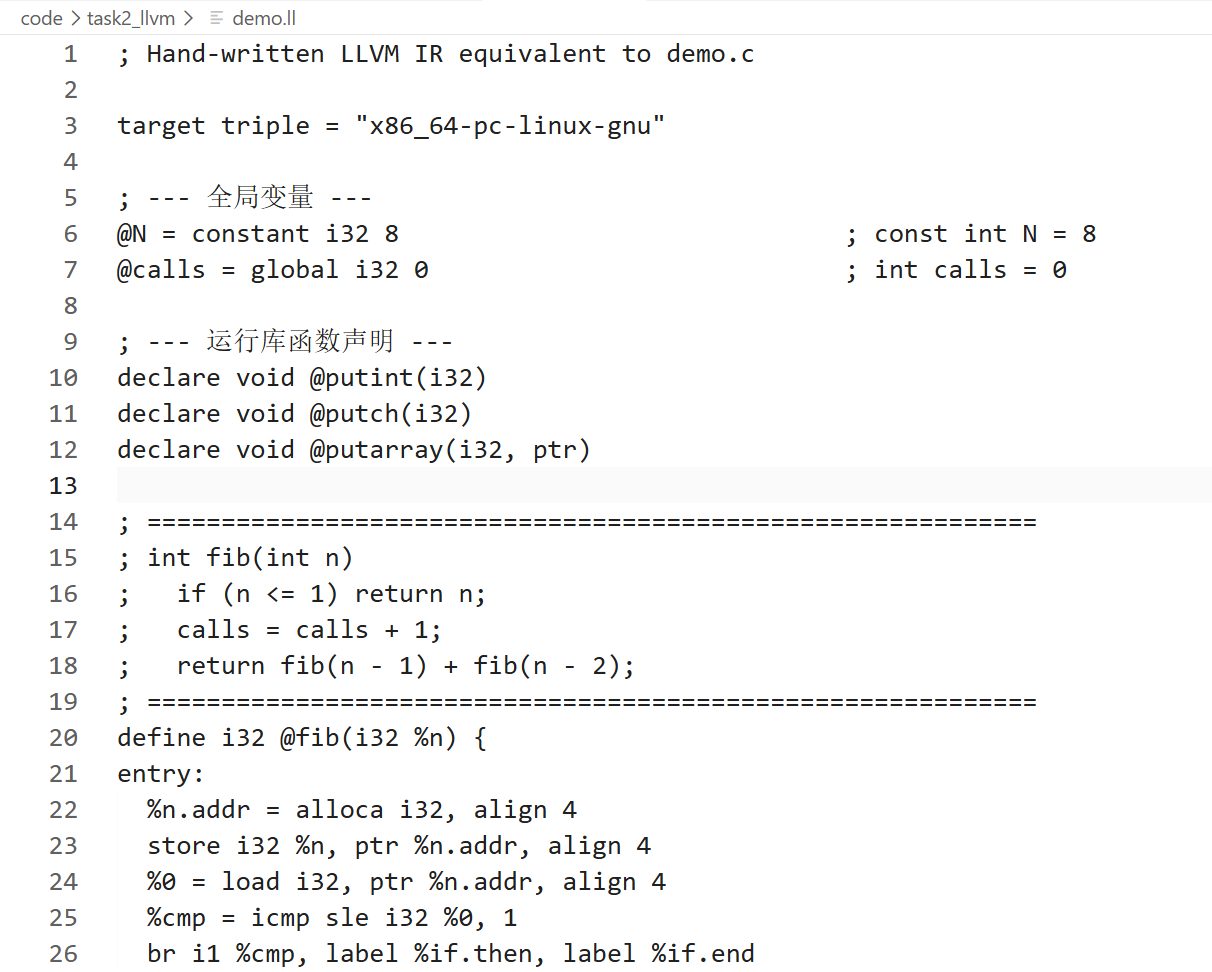
\includegraphics[width=0.92\textwidth]{task2_llvm/2.png}
  \caption{手写 demo.ll 的开头部分}
  \label{fig:llvm-demoll}
\end{figure}

\hfour{10、手写 IR 中容易出错的地方}

把本次手写过程中真正遇到、或容易遇到的错误归纳如表~\ref{tab:llverr} 所示。

\begin{table}[H]
  \centering
  \small
  \setlength{\tabcolsep}{4pt}
  \begin{tabular}{>{\centering\arraybackslash}p{3.2cm}>{\centering\arraybackslash}p{5.0cm}>{\centering\arraybackslash}p{5.8cm}}
    \toprule
\headcol 问题 & \headcol 现象 & \headcol 正确做法 \\
    \midrule
GEP 索引类型不对 & llvm-as 报类型错误 & 循环变量须先 sext i32 ... to i64 再作索引 \\
    基本块缺少终结指令 & 报 “block must be terminated by a terminator” & 每个块的末尾必须是 br / ret 之一 \\
    把函数参数当变量改写 & 报 SSA 值不可重复赋值 & 先 alloca 到栈上，用 load/store 读写 \\
    忘记数组退化 & call ... @putarray 实参类型不符 & 用 GEP 取首元素地址再传入 \\
    全局量与局部量前缀混淆 & 名字解析失败 & 全局用 @，局部用 \%，不可混用 \\
    指令漏写类型 & 报 “expected type” 之类错误 & load/store/icmp/call 都要写明操作数类型 \\
    除法选错指令 & 结果不符（但能通过语法检查） & 有符号用 sdiv/srem，无符号用 udiv/urem \\
    \bottomrule
\end{tabular}
  \caption{手写 LLVM IR 的常见错误}
  \label{tab:llverr}
\end{table}

关于最后一条尤其值得警惕：\textbf{类型错误会被 llvm-as 拦住，而语义错误（如该用 sdiv 却用了 udiv、下标差一位）不会被拦住}，只能靠运行结果比对来发现。因此本实验始终坚持“语法检查 + 运行比对”两道关，后者由后续的 diff 完成。

\subsubsection{编译与验证}

\hfour{1、语法检查}

\begin{lstlisting}[language=bash]
$ cd /mnt/d/OS_CS/compiler-system-labs/lab1/code/task2_llvm
$ llvm-as demo.ll -o /dev/null && echo "llvm-as: OK"
llvm-as: OK
\end{lstlisting}

llvm-as 在把文本 IR 汇编为位码时会完成全部语法与类型检查，能通过即说明 IR 本身是合法的；若存在漏写类型、GEP 索引宽度不对、基本块缺少终结指令等问题，都会在这一步被拦下。

\hfour{2、链接运行库并编译运行}

\begin{lstlisting}[language=bash]
$ clang demo.ll sylib.c -o demo_ir
$ ./demo_ir
5
5: 0 1 1 2 3
5
14
7
\end{lstlisting}

clang 识别到 demo.ll 是文本中间代码，将其编译后与 sylib.c 一起链接。终端回显如图~\ref{fig:llvm-run} 所示，运行输出与第三章给出的预期结果完全一致。

\begin{figure}[H]
  \centering
  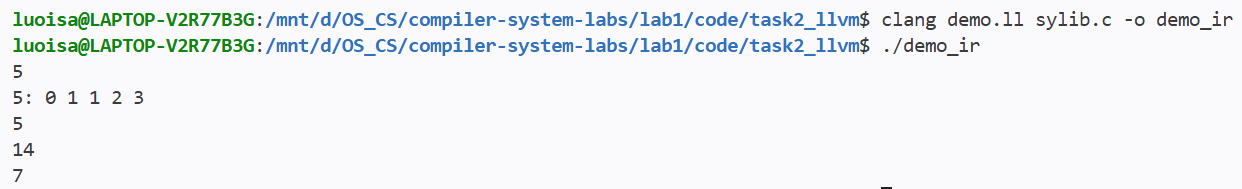
\includegraphics[width=0.92\textwidth]{task2_llvm/3.png}
  \caption{用 clang 将 demo.ll 与 sylib.c 一起编译并运行，输出与预期一致}
  \label{fig:llvm-run}
\end{figure}

\hfour{3、与 C 版本逐字节比对}

\begin{lstlisting}[language=bash]
$ ./demo_ir > actual.txt
$ diff expected.txt actual.txt && echo "MATCH"
MATCH
\end{lstlisting}

先用 GCC 编译 demo.c 生成期望输出 expected.txt，再用 diff 逐字节比对两个程序的输出，结果完全一致，如图~\ref{fig:llvm-diff} 所示。\textbf{这比“肉眼看输出差不多”可靠得多}：哪怕只差一个空格或一个换行，diff 也会报出来。至此可以确认手写 IR 与 SysY 源程序语义等价。

\begin{figure}[H]
  \centering
  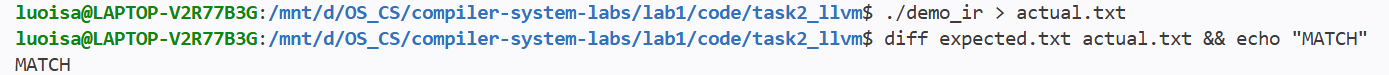
\includegraphics[width=0.92\textwidth]{task2_llvm/4.png}
  \caption{diff 逐字节比对 IR 版输出与 C 版期望输出，无差异并打印 MATCH}
  \label{fig:llvm-diff}
\end{figure}

\subsubsection{与 Clang 自动生成 IR 的对照}

手写 IR 的价值在于“读懂”中间语言；而要看清编译器真正的高明之处，则须与它自动生成的 IR 对照。用 Clang 分别在两个优化级别下生成对照版本：

\begin{lstlisting}[language=bash]
$ clang -O0 -emit-llvm -S -include syhdr.h demo.c -o auto_O0.ll   # 196 行
$ clang -O2 -emit-llvm -S -include syhdr.h demo.c -o auto_O2.ll   # 97 行
\end{lstlisting}

三版 IR 的规模为：手写 demo.ll 209 行，自动 -O0 版 196 行，自动 -O2 版 97 行。三版文件在编辑器中的对照如图~\ref{fig:llvm-three} 所示。

\begin{figure}[H]
  \centering
  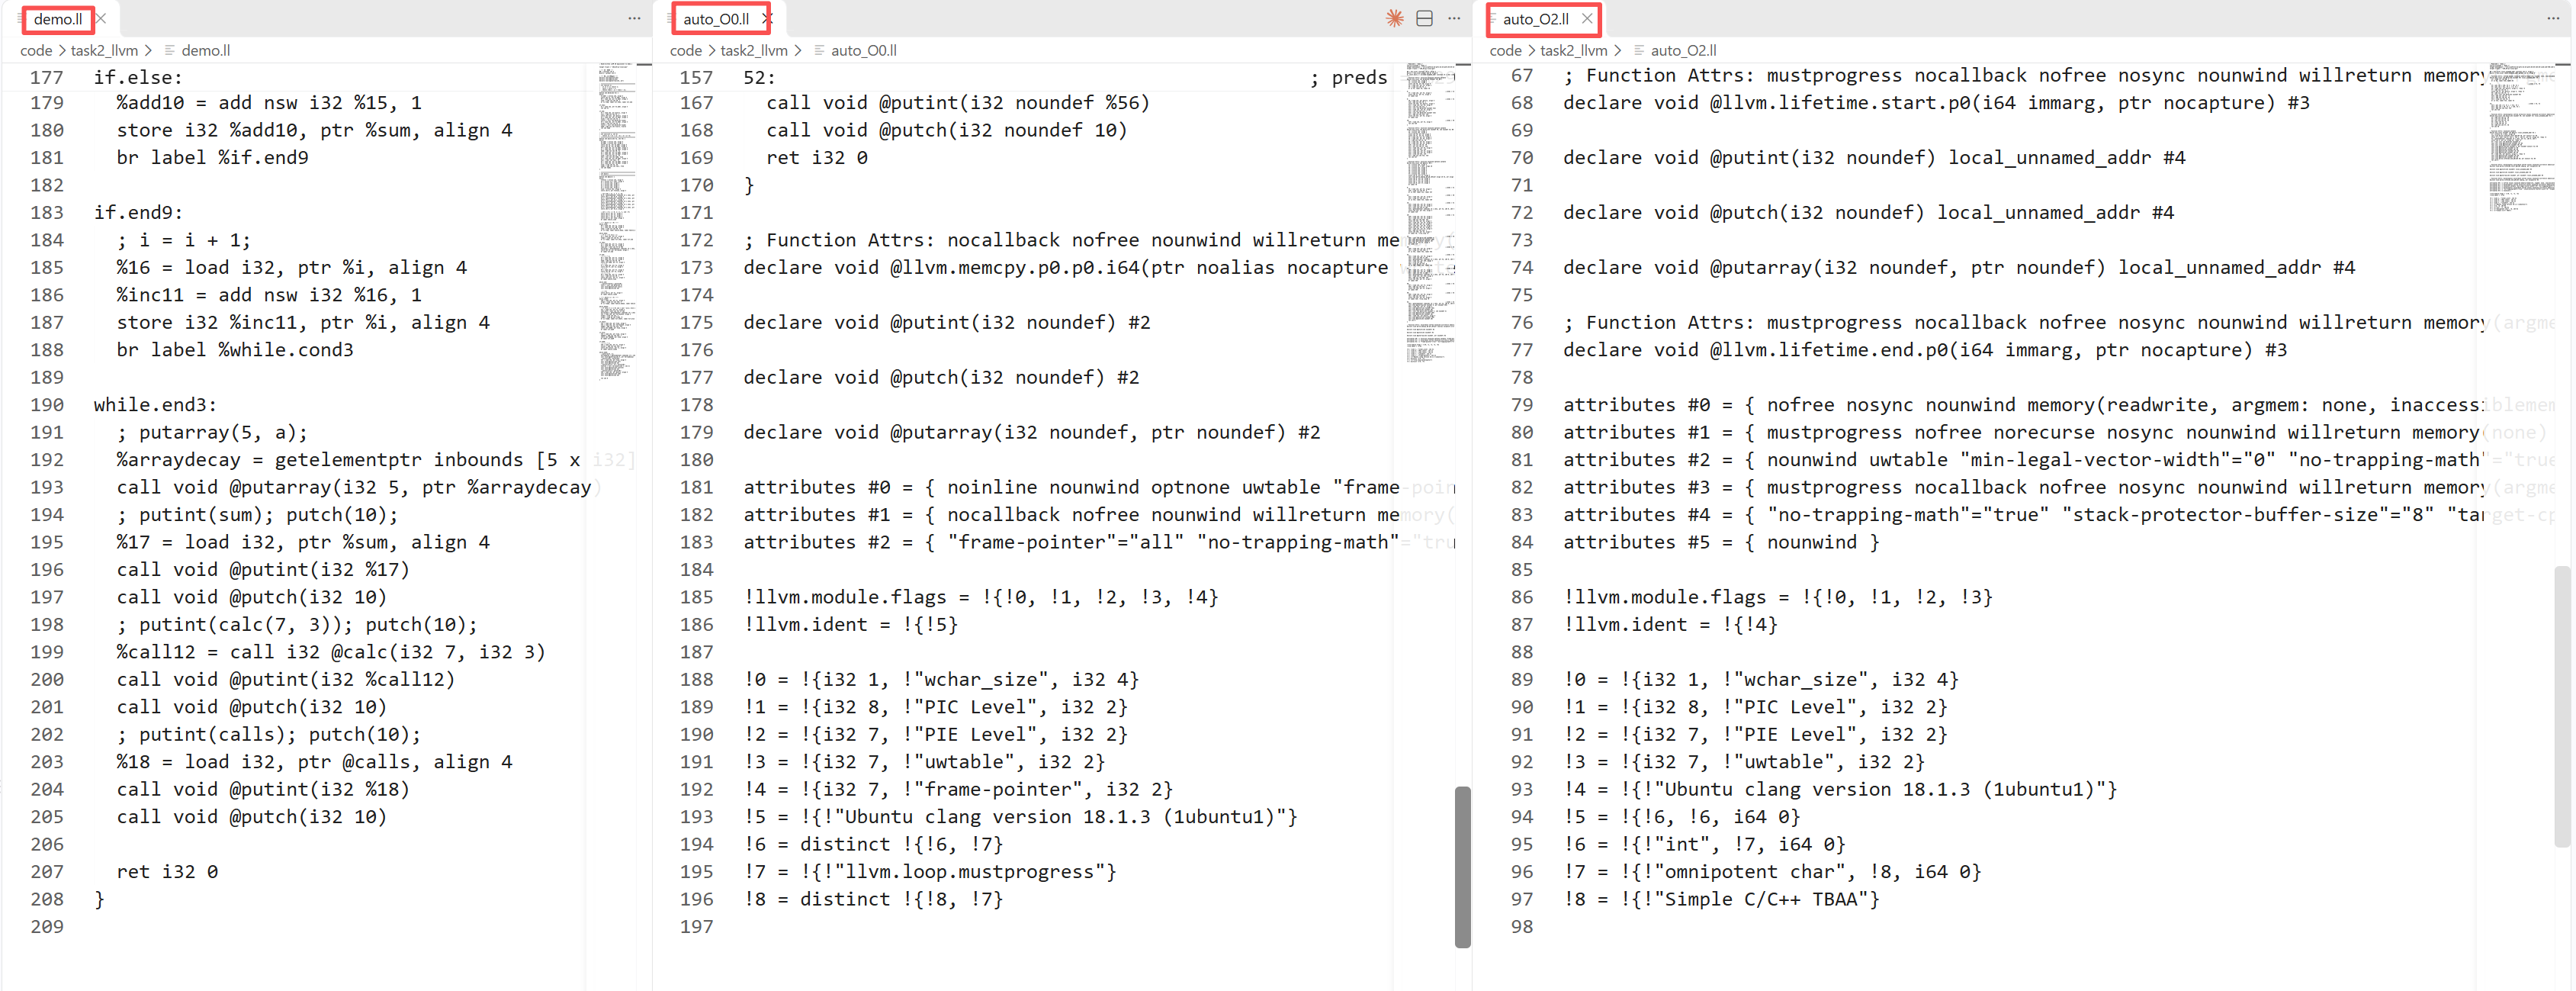
\includegraphics[width=0.95\textwidth]{task2_llvm/5.png}
  \caption{三版 IR 对照（从左到右）：手写 demo.ll、auto\_O0.ll、auto\_O2.ll 的末尾部分，具体代码见仓库}
  \label{fig:llvm-three}
\end{figure}

\hfour{1、手写版与 Clang -O0 版的对照}

两者的\textbf{整体结构高度一致}，都可以一眼认出“三段式”：alloca 局部变量、load/store 读写、基本块之间跳转。这印证了手写 IR 所采用的风格确实就是 -O0 的风格。差异则集中在若干细节，如表~\ref{tab:hvo0} 所示。

\begin{table}[H]
  \centering
  \small
  \setlength{\tabcolsep}{4pt}
  \begin{tabular}{>{\centering\arraybackslash}p{2.4cm}>{\centering\arraybackslash}p{5.0cm}>{\centering\arraybackslash}p{6.6cm}}
    \toprule
\headcol 方面 & \headcol 手写 demo.ll & \headcol Clang -O0（auto\_O0.ll） \\
    \midrule
函数属性 & 无 & 带 noinline nounwind optnone uwtable、frame-pointer=all \\
    返回值 & 直接 ret 具体值 & 先 store 到 \%retval 槽位，最后统一 load 后 ret \\
    const int N & 从全局 @N 加载 & \textbf{直接内联为立即数 8}（icmp slt i32 \%9, 8） \\
    数组初始化 & 5 组 getelementptr + store & 生成私有常量 @\_\_const.main.a，再 memcpy 20 字节 \\
    块命名 & while.cond、if.then 等语义化名字 & 一律数字编号（6、8、19…） \\
    指针类型 & 显式 ptr & 显式 ptr，但附带 noundef、align 等属性 \\
    \bottomrule
\end{tabular}
  \caption{手写 demo.ll 与 Clang -O0 版的差异}
  \label{tab:hvo0}
\end{table}

其中最有意思的一条是\textbf{常量 N 的处理}。C 语言中 const 只是“只读”语义，编译器在已知其初始值的情况下可以直接把 8 写进比较指令，而不必真的去内存里读：

\begin{lstlisting}[language=LLVM]
; auto_O0.ll 中 main 的循环条件
  %9 = load i32, ptr %3, align 4
  %10 = icmp slt i32 %9, 8        ; N 已被内联为立即数 8
\end{lstlisting}

而在手写版中，N 仍是那条 load i32, ptr @N。两者语义相同，但后者在 -O0 下会多一次访存。另外，数组初始化之所以从“5 组 store”变成了“@\_\_const.main.a + memcpy”，是因为对较大的初始化列表，编译器倾向于把常量整块放进只读区再一次性复制——memcpy 中的 i64 20 就是 5 个 i32 的字节数。

最后，-O0 生成的每个函数都带有 optnone 属性，其含义是“\textbf{不要对这个函数做任何优化}”。这一属性会带来一个容易被误解的现象：即使事后用 opt -O2 去处理这份 IR，循环也不会被优化掉，因为 optnone 已经明确禁止了优化（第二章任务一中对这一点已有直接观察）。

\hfour{2、Clang -O0 与 Clang -O2 对照：优化做了什么}

从 196 行骤减到 97 行，优化做的事可以归纳为四件。

\textbf{其一，消除栈上分配，转为 SSA 值。} -O0 中 calc 有多条 alloca 与十余次 load/store；-O2 中它们全部消失，函数变成一串纯运算：

\begin{lstlisting}[language=LLVM]
define dso_local i32 @calc(i32 noundef %0, i32 noundef %1) {
  %3 = add nsw i32 %1, %0
  %4 = sub nsw i32 %0, %1
  %5 = mul nsw i32 %3, %4
  %6 = sdiv i32 %5, %1
  %7 = srem i32 %0, %1
  %8 = add nsw i32 %7, %6
  ret i32 %8
}
\end{lstlisting}

这就是 4.1.3 节所说的“内存中的变量被提升为寄存器中的 SSA 值”。main 中也只剩 \%1 = alloca [5 x i32] 一条——因为数组确实需要真实的内存。

\textbf{其二，main 中的两个循环被完全求值（循环展开 + 常量折叠）。} 优化器发现两个循环的输入都是编译期常量，索性在编译期把结果算了出来：

\begin{lstlisting}[language=LLVM]
define dso_local noundef i32 @main() {
  %1 = alloca [5 x i32], align 16
  call void @llvm.lifetime.start.p0(i64 20, ptr nonnull %1)
  store <4 x i32> <i32 0, i32 1, i32 1, i32 2>, ptr %1, align 16   ; a[0..3]
  %2 = getelementptr inbounds [5 x i32], ptr %1, i64 0, i64 4
  store i32 3, ptr %2, align 16                                     ; a[4] = 3
  ...
  call void @putint(i32 noundef 5)                                  ; sum 被折叠为 5
  ...
  call void @putint(i32 noundef 14)                                 ; calc(7,3) 被折叠为 14
\end{lstlisting}

对照第三章的手工验算：a = \{0,1,1,2,3\}（于是 store <4 x i32> <0,1,1,2> 加一条 store 3）、sum = 5、calc(7,3) = 14——\textbf{优化器算出的结果与人工笔算完全一致}。原来两个完整的循环，如今只剩下两条 store 和几个常量实参；while 与 if 的影子荡然无存。此外 main 中用 store <4 x i32> 一次写入 4 个元素，用到了向量类型的指令。

\textbf{其三，fib 中出现了 PHI 节点，且双重递归被改写。} 这是三版对照中最值得玩味的一处：

\begin{lstlisting}[language=LLVM]
define dso_local i32 @fib(i32 noundef %0) {
  %2 = icmp slt i32 %0, 2
  br i1 %2, label %13, label %3

3:                                    ; preds = %1, %3
  %4 = phi i32 [ %10, %3 ], [ %0, %1 ]      ; 当前的 n
  %5 = phi i32 [ %11, %3 ], [ 0, %1 ]       ; 累加值
  %6 = load i32, ptr @calls, align 4, !tbaa !5
  %7 = add nsw i32 %6, 1
  store i32 %7, ptr @calls, align 4, !tbaa !5
  %8 = add nsw i32 %4, -1
  %9 = tail call i32 @fib(i32 noundef %8)   ; 仍保留一次递归
  %10 = add nsw i32 %4, -2
  %11 = add nsw i32 %9, %5
  %12 = icmp ult i32 %4, 4
  br i1 %12, label %13, label %3
\end{lstlisting}

要点如下：

\begin{itemize}
  \item \textbf{PHI 节点出现了。} \%4 = phi i32 [ \%10, \%3 ], [ \%0, \%1 ] 表示：从块 \%3 自循环进入时取上一轮的 \%10，从入口 \%1 进入时取参数 \%0。\textbf{在 -O0 里靠 alloca 反复读写同一块内存实现的东西，在这里变成了 PHI 节点在控制流汇合处挑选取值。} 这正是 SSA 形式的标志。手写 IR 时刻意回避的那部分内容，在优化后的代码里必然要出现。
  \item \textbf{双重递归被改写为“单重递归 + 一个循环”。} 原式的两次递归调用，如今只剩 tail call i32 @fib(i32 \%8) 一次，另一次被改写成了循环中的累加（\%5 记录累加值，\%11 = add \%9, \%5）。编译器认出“第二次调用的结果可以直接累加”，从而把树形递归压成了一条链。
  \item \textbf{tail call} 表示尾调用，后端可据此省去新的栈帧。
  \item \textbf{icmp ult} 中 ult 是“无符号小于”，这里用于判断循环是否继续（编译器已知 n 非负，故用无符号比较亦无歧义）。
\end{itemize}

\textbf{其四，属性与元信息更丰富。} -O2 版为每个函数加上了 nofree、nosync、norecurse、willreturn、memory(none) 等属性，并插入了 llvm.lifetime.start/end 生命周期标记（告知后端数组的存活区间，用于栈槽复用），以及 TBAA（类型别名分析）元信息 !tbaa。这些都是优化器与后端使用的“附加情报”，源码与手写 IR 中都不会有。

\subsection{三版 IR 对比汇总}

把三版 IR 的各项特征汇总于表~\ref{tab:threeir}。

\begin{table}[H]
  \centering
  \small
  \setlength{\tabcolsep}{4pt}
  \begin{tabular}{>{\centering\arraybackslash}p{2.4cm}>{\centering\arraybackslash}p{3.7cm}>{\centering\arraybackslash}p{3.9cm}>{\centering\arraybackslash}p{4.0cm}}
    \toprule
\headcol 维度 & \headcol 手写 demo.ll & \headcol Clang -O0 & \headcol Clang -O2 \\
    \midrule
行数 & 209 & 196 & 97 \\
    局部变量表示 & alloca + load/store & alloca + load/store & SSA 值（仅数组保留 alloca） \\
    PHI 节点 & 无 & 无 & \textbf{有}（fib） \\
    const N & 从 @N 加载 & 内联为立即数 8 & 内联为立即数 8 \\
    数组初始化 & 5 组 GEP + store & 私有常量 + memcpy & 向量 store 一次写入 \\
    循环 & 运行时执行 & 运行时执行 & \textbf{编译期求值}（main） \\
    递归 & 原始双重递归 & 原始双重递归 & \textbf{改为单递归 + 循环} \\
    函数属性 & 无 & optnone、frame-pointer=all & nofree、willreturn 等 \\
    辅助元信息 & 无 & 少量 & lifetime、tbaa \\
    \bottomrule
\end{tabular}
  \caption{手写版、Clang -O0 版与 Clang -O2 版 IR 对比}
  \label{tab:threeir}
\end{table}

三者描述的是\textbf{同一个程序}，但形态迥异：手写版与 -O0 版是“人可以照着写出来”的直白形式，而 -O2 版是“只有机器才看得懂”的优化结果。\textbf{这一对照恰好说明：中间表示既是编译器内部的工作语言，也是不同优化阶段之间传递信息的载体。}

\subsection{小结}

\begin{enumerate}[1.]
  \item \textbf{手写 IR 必须靠“比对”而非“目测”来验证语义等价。} 类型错误会被 llvm-as 拦下，但语义错误（如该用 sdiv 却写成 udiv）能通过语法检查。本次用 GCC 生成期望输出再与 IR 版 diff 逐字节比对，才可靠确认等价性。

  \item \textbf{alloca 是理解 LLVM IR 与优化的入口。} -O0 下每个局部变量对应一条 alloca，读写靠 load/store，语义明确易手写；而优化器消除 alloca 后需补上 PHI 节点，"从内存变量到寄存器值"的转变是 LLVM 优化的核心一步。

  \item \textbf{控制流结构在 IR 中被抹平为条件跳转。} while、if 在 IR 中都变成“比较 + br'的组合，高级语言的结构化特征到中间表示层已转化为控制流图。

  \item \textbf{优化前后的差距可用数字衡量。} -O0 到 -O2，IR 行数由 196 降至 97，循环被整体求值、访存大幅减少，同一段源码在中间表示层面留下巨大鸿沟。
\end{enumerate}

\section{任务三：RISC-V 汇编编程}

\subsection{程序一：斐波那契数列与数组运算}

\subsubsection{汇编程序编写思路}

我是对照着 SysY 源程序逐段编写这份汇编的，整体上遵循先定数据布局、再定寄存器分工、最后逐语句翻译的顺序，具体思路如下。

\hfour{1. 全局数据的段归属}

源程序有两个全局对象：N 被 const 修饰、内容不可变，我把它放进只读数据段 .rodata，直接用 .word 8 静态嵌入；calls 是可写变量并且初值为 0，放进 .bss 段，用 .zero 4 只预留空间，由加载器在程序启动时清零。两者都用 .align 2 对齐到 4 字节，与 int 的自然对齐一致，因为后续要用 lw 访问它们。

\hfour{2. 栈帧的分配}

每个函数进入时先把 sp 下移，为自己开辟一块固定的栈帧；函数出口再上移相同的字节数收回，栈帧大小保持 16 字节对齐。本程序中 fib 用了 32 字节、calc 用了 16 字节、main 用了 80 字节。栈帧内部我按先高地址放保存寄存器、再放局部变量的顺序排布，让 sp 本身就可以直接充当数组的基址，这样就能省掉一次取址运算。

\hfour{3. 寄存器分工}

遵循 RISC-V 约定：a0–a7 传参与返回，ra 存返回地址，sp 为栈指针，t0–t6 作临时量，s1–s5 作变量。以 main 为例，我把 i、x、y、t、sum 五个局部变量分别固定在 s1–s5 中，这样能明显减少访存指令，但是在函数入口必须把用到的 s 寄存器全部压栈保护。

\hfour{4. 关键语句的翻译策略}

\begin{itemize}
  \item if (n <= 1)：RISC-V 有 blt、ble、bgt、bge 四条比较跳转指令，直接用 ble 判断也可以；这里我选择把条件取反写成“若 n > 1 则进入递归分支”，用 bgt 完成判断，为的是让 n <= 1 这个最短的基准情形顺序执行、不必再跳一次。
  \item calls = calls + 1：全局变量不能用 sp 加偏移直接访问，需要先 lla 取地址再 lw/sw。
  \item a[i] = x：数组下标访问要拆成\textbf{基址 + 下标 $\times$ 4}两步。因为 int 占 4 字节，乘以 4 可以用 slli 左移 2 位代替；main 中数组位于栈帧最低处，sp 就是基址，所以一条 add 即可得到元素地址。
  \item a[i] \% 2 == 0：对非负整数而言，取最低位与取模 2 是等价的，因此我们选择用 andi t4, t3, 1 加 bnez 判断奇偶。
  \item fib(n-1) + fib(n-2)：第一次递归调用的结果必须保存在被调用者保存寄存器 s1 中，因为第二次 call fib 完全可能覆写 a0 这类调用者保存寄存器，把结果留在 a0 里会出错。
\end{itemize}

\hfour{5. 循环的组织方式}

我把判断条件统一放在循环体开头，这样是为了条件判断与循环体在汇编中的顺序同源程序一致，但是代价是每轮多一条回跳指令，效率略低，但对于本程序的规模是可以接受的。

依据上述思路，我最终编写出的汇编程序 demo.s 整体由表~\ref{tab:demoscomp} 所示的几部分组成。

\begin{table}[H]
  \centering
  \small
  \setlength{\tabcolsep}{4pt}
  \begin{tabular}{>{\centering\arraybackslash}p{2.6cm}>{\centering\arraybackslash}p{6.2cm}>{\centering\arraybackslash}p{5.2cm}}
    \toprule
\headcol 部分 & \headcol 内容 & \headcol 对应源程序 \\
    \midrule
文件头 & 文件说明注释与汇编器指令 & — \\
    全局数据 & 常量 N、变量 calls & const int N = 8; / int calls = 0; \\
    函数 fib & 递归求斐波那契 & int fib(int n) \\
    函数 calc & 四则运算与取余 & int calc(int a, int b) \\
    函数 main & 数组、双循环、调用与输出 & int main() \\
    收尾标识 & .ident 与栈属性标记 & — \\
    \bottomrule
\end{tabular}
  \caption{手写汇编程序 demo.s 的组成}
  \label{tab:demoscomp}
\end{table}

demo.s 的全文整体缩略视图如图~\ref{fig:riscv-demos} 所示。

\begin{figure}[H]
  \centering
  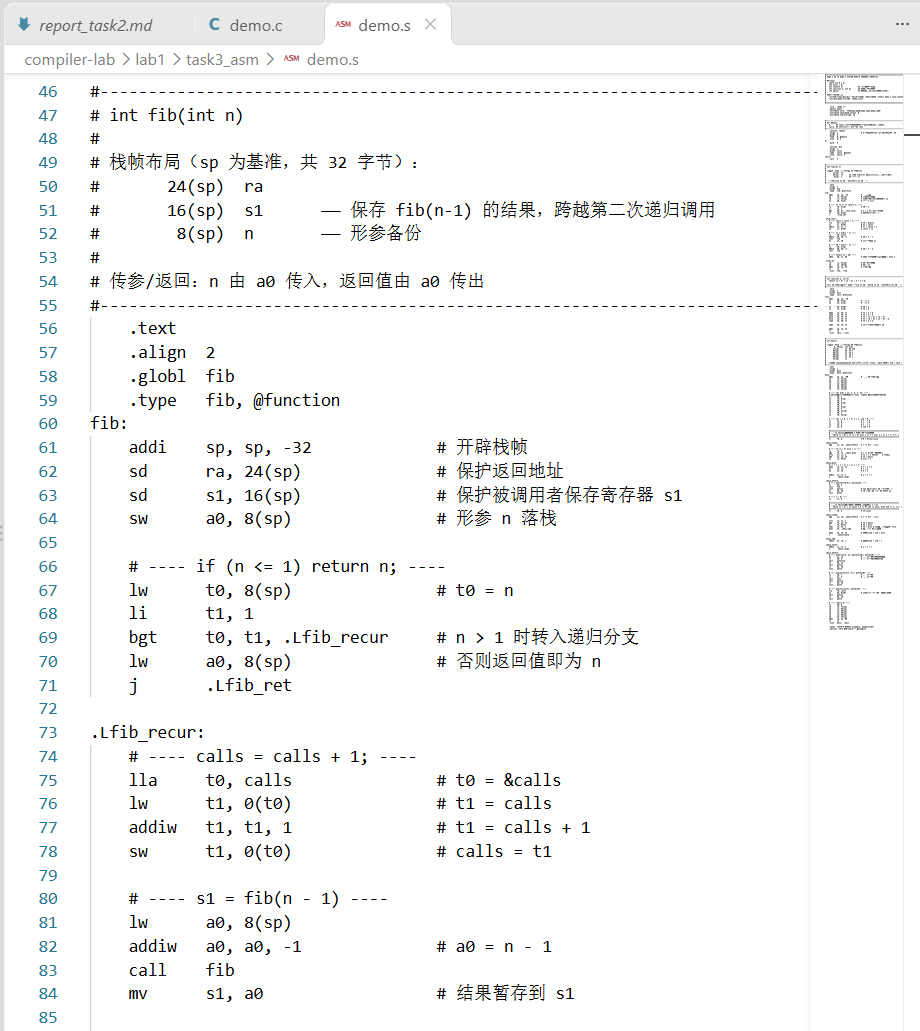
\includegraphics[width=0.92\textwidth]{task2_riscv/截图3.png}
  \caption{手写汇编程序 demo.s 全文（编辑器整体缩略视图）}
  \label{fig:riscv-demos}
\end{figure}

\subsubsection{汇编程序分析}

下面分块给出编写的汇编程序并做详细解释。

\hfour{1. 文件头与汇编器指令}

\begin{lstlisting}[language=riscv]
    .file   "demo.s"
    .option nopic
    .attribute arch, "rv64i2p1_m2p0_a2p1_f2p2_d2p2_c2p0"
    .attribute unaligned_access, 0
    .attribute stack_align, 16
\end{lstlisting}

前几行是给汇编器和链接器看的元信息，本身不产生任何机器指令。

\begin{itemize}
  \item .file "demo.s"：声明本汇编文件的名字，调试时可用它在符号表里定位到源文件。
  \item .option nopic：告诉汇编器不必按位置无关代码的规则生成重定位信息，这是因为我们的程序最终以静态方式链接。
  \item .attribute arch, ...：声明目标架构。rv64i 是 64 位基础整数指令集；m 提供乘除法扩展，对应后文用到的 mulw、divw、remw；a 是原子指令扩展；f、d 分别是单精度和双精度浮点扩展；c 是压缩指令扩展。
  \item .attribute unaligned\_access, 0：禁止未对齐访存。任何跨越自然边界的访问都会触发异常。
  \item .attribute stack\_align, 16：规定栈指针始终保持 16 字节对齐。这是 RV64 ABI 的硬性要求，因为 sd/ld 这类 64 位访存需要自然对齐，而且后续若引入浮点参数传递，也会依赖这个约定。
\end{itemize}

\hfour{2. 全局常量与全局变量}

\begin{lstlisting}[language=riscv]
    .section .rodata
    .align  2                       # 4 字节对齐，与 int 的自然对齐一致
    .globl  N
    .type   N, @object
    .size   N, 4
N:
    .word   8

    .section .bss
    .align  2
    .globl  calls
    .type   calls, @object
    .size   calls, 4
calls:
    .zero   4
\end{lstlisting}

\begin{itemize}
  \item .section .rodata：切换到只读数据段。N 是 const，取值编译期就已确定，因此以 .word 8 的形式直接嵌入目标文件，运行时不需要任何初始化指令。
  \item .globl N：把 N 声明为全局符号，使其在链接后仍对其它目标文件可见；.type N, @object 与 .size N, 4 则告诉链接器 N 是一个占 4 字节的数据对象、不是函数，便于链接期做类型检查。
  \item .align 2：把当前地址对齐到 $2^2=4$ 字节边界。int 宽 4 字节，对齐之后一条 lw 就能在一个总线周期内取到完整的一个字。
  \item N: .word 8：定义标签 N，并在该位置放一个 32 位的字，值为 8。
  \item .section .bss 中的 calls 处理方式完全相同，但它被放进 .bss 段，链接时只记录它需要 4 字节空间（.zero 4），不占用可执行文件的体积，程序启动时由加载器统一清零。
\end{itemize}

\hfour{3. 函数 fib}

\textbf{（1）函数入口与栈帧布局。}

\begin{lstlisting}[language=riscv]
    .text
    .align  2
    .globl  fib
    .type   fib, @function
fib:
    addi    sp, sp, -32             # 开辟栈帧
    sd      ra, 24(sp)              # 保护返回地址
    sd      s1, 16(sp)              # 保护被调用者保存寄存器 s1
    sw      a0, 8(sp)               # 形参 n 落栈
\end{lstlisting}

.text 切回代码段，.align 2 把函数入口对齐到 4 字节边界。fib 的栈帧只有 32 字节，内部布局如下：

\begin{lstlisting}
    sp+24   ra          返回地址
    sp+16   s1          跨调用暂存的中间结果
    sp+8    n           形参备份
\end{lstlisting}

进入函数后先 addi sp,sp,-32 把栈指针下移，为调用开辟空间；sd ra,24(sp) 保存返回地址；sd s1,16(sp) 保存 s1，因为下面要用它暂存中间结果，s1 属于被调用者保存寄存器，按约定必须由我们自己负责保护。最后 sw a0,8(sp) 把按约定传入 a0 的形参 n 备份到栈上，此后每次都从 sp+8 读取。

\textbf{（2）实现 if (n <= 1) return n;。}

\begin{lstlisting}[language=riscv]
    lw      t0, 8(sp)               # t0 = n
    li      t1, 1
    bgt     t0, t1, .Lfib_recur     # n > 1 时转入递归分支
    lw      a0, 8(sp)               # 否则返回值即为 n
    j       .Lfib_ret
\end{lstlisting}

RISC-V 的分支指令有 blt（小于）、ble（小于等于）、bgt（大于）、bge（大于等于）四条，直接用 ble 判断 n <= 1 也可以；这里改用 bgt，把条件取反成 n > 1 时跳入递归分支，好处是基准情形（直接返回 n）落在顺序执行的位置上，整个函数少一次跳转。当 n <= 1 时，顺序执行 lw a0,8(sp) 把 n 送入返回寄存器 a0，再 j .Lfib\_ret 跳到统一出口。

\textbf{（3）实现 calls = calls + 1;。}

\begin{lstlisting}[language=riscv]
.Lfib_recur:
    lla     t0, calls               # t0 = &calls
    lw      t1, 0(t0)               # t1 = calls
    addiw   t1, t1, 1               # t1 = calls + 1
    sw      t1, 0(t0)               # calls = t1
\end{lstlisting}

calls 是全局变量，需要先取得它的地址。lla（load local address）是加载本地符号地址的伪指令，把 calls 的地址装入 t0；随后 lw 取值、addiw 加 1、sw 写回。这里用 addiw 而不是 addi，是因为 calls 是 32 位 int；addiw 只做 32 位加法并自动把结果符号扩展为 64 位，正好符合 int 的运算语义，可以省去额外的 sext.w。

\textbf{（4）实现 return fib(n - 1) + fib(n - 2);。}

\begin{lstlisting}[language=riscv]
    lw      a0, 8(sp)
    addiw   a0, a0, -1              # a0 = n - 1
    call    fib
    mv      s1, a0                  # 结果暂存到 s1

    lw      a0, 8(sp)
    addiw   a0, a0, -2              # a0 = n - 2
    call    fib

    addw    a0, s1, a0              # addw 自带符号扩展，无需再 sext.w
\end{lstlisting}

这段是 fib 的核心。第一次递归前，先把 n - 1 装入 a0，然后 call fib。call 是 auipc 与 jalr 组合的伪指令，它会把下一条指令的地址写入 ra 再跳转，返回后结果位于 a0，紧接着 mv s1,a0 把它转移到 s1。

a0 属于调用者保存寄存器，也就是说被调用的函数可以随意覆写它、不需要恢复。如果直接把 fib(n-1) 的结果留在 a0 里就去执行第二次 call fib，那么返回时这个值很可能已经被破坏，因此必须把它转移到被调用者保存寄存器 s1 中暂存。\textbf{这正是为什么要区分 caller-saved 与 callee-saved 两组寄存器最直观的例子：跨函数调用存活的中间结果，只能放在后者里。}

第二次递归以同样的方式求出 fib(n-2)，返回后 a0 中是它的结果，s1 中是 fib(n-1) 的结果，因此只需一条 addw a0,s1,a0 就完成了加法。这里没有再补 sext.w，是因为 addw 的语义本身就是做 32 位加法并把结果符号扩展写入 64 位寄存器，扩展已经隐含在内了。

\textbf{（5）统一出口。}

\begin{lstlisting}[language=riscv]
.Lfib_ret:
    ld      ra, 24(sp)              # 恢复返回地址
    ld      s1, 16(sp)              # 恢复 s1
    addi    sp, sp, 32              # 回收栈帧
    jr      ra
\end{lstlisting}

.Lfib\_ret 被两条路径共用：n <= 1 时 a0 中已经是 n，递归分支结束时 a0 中是两项之和，两种情形都不需要额外处理即可直接返回。随后按与压栈相反的顺序恢复 ra 与 s1，addi sp,sp,32 回收栈帧，最后 jr ra 跳回调用者。

\hfour{4. 函数 calc}

\textbf{（1）入口与参数保存。}

\begin{lstlisting}[language=riscv]
    .text
    .align  2
    .globl  calc
    .type   calc, @function
calc:
    addi    sp, sp, -16
    sw      a0, 0(sp)               # 备份 a
    sw      a1, 4(sp)               # 备份 b
\end{lstlisting}

calc 内部不调用任何其它函数，因此不需要保护 ra，也不需要使用任何 s 寄存器，只需要 8 字节来安放形参即可；为了满足栈指针 16 字节对齐的要求，栈帧取 16 字节。参数传递上，第一个参数 a 由 a0 传入，第二个参数 b 由 a1 传入。

\textbf{（2）实现 (a + b) * (a - b) / b + a \% b。}

\begin{lstlisting}[language=riscv]
    lw      t0, 0(sp)               # t0 = a
    lw      t1, 4(sp)               # t1 = b

    addw    t2, t0, t1              # t2 = a + b
    subw    t3, t0, t1              # t3 = a - b
    mulw    t2, t2, t3              # t2 = (a + b) * (a - b)
    divw    t3, t2, t1              # t3 = (a + b) * (a - b) / b
    remw    t4, t0, t1              # t4 = a % b

    addw    a0, t3, t4              # 结果放入返回寄存器 a0
\end{lstlisting}

这段代码严格按 C 语言的运算符优先级逐步求值。RISC-V 的算术指令是三地址格式——两个源寄存器加一个目的寄存器，因此每一步中间结果都要占用一个临时寄存器，这里依次使用了 t2、t3、t4。addw/subw/mulw/divw/remw 这一组带 w 后缀的指令都按 32 位字运算并自动做符号扩展，与 C 语言中 int 的语义严格对应；相比之下，不带 w 的 add、sub 是做 64 位运算的，用在这里会导致高位出现非预期的数值。最后把结果放入 a0，恢复栈指针后 jr ra 返回。

\hfour{5. 函数 main}

main 是本程序中最长的一个函数。为便于分析，下面按功能分成若干小块。

\textbf{（1）栈帧与寄存器保护。}

\begin{lstlisting}[language=riscv]
main:
    addi    sp, sp, -80             # 开辟 80 字节栈帧
    sd      ra, 72(sp)
    sd      s1, 64(sp)
    sd      s2, 56(sp)
    sd      s3, 48(sp)
    sd      s4, 40(sp)
    sd      s5, 32(sp)
\end{lstlisting}

main 内部要调用 fib、calc、putint 等函数，所以既要保护 ra，也要把用到的全部 s 寄存器压栈保存。栈帧共 80 字节，布局如下：

\begin{lstlisting}
    sp + 0  ...  sp + 19    int a[5]        （20 字节）
    sp + 32               s5  —— sum
    sp + 40               s4  —— t
    sp + 48               s3  —— y
    sp + 56               s2  —— x
    sp + 64               s1  —— i
    sp + 72               ra
\end{lstlisting}

把数组安排在栈帧最低处、四字节对齐，使得 sp 本身就直接充当了数组的基址，后面访问 a[i] 时无需再单独计算基址，一条 add 就能得到元素地址。

\textbf{（2）初始化数组与局部变量。}

\begin{lstlisting}[language=riscv]
    li      t0, 1
    sw      t0, 0(sp)
    li      t0, 2
    sw      t0, 4(sp)
    li      t0, 3
    sw      t0, 8(sp)
    li      t0, 4
    sw      t0, 12(sp)
    li      t0, 5
    sw      t0, 16(sp)

    li      s1, 0                   # i   = 0
    li      s2, 0                   # x   = 0
    li      s3, 1                   # y   = 1
    li      s5, 0                   # sum = 0
\end{lstlisting}

数组 a 的初值 \{1,2,3,4,5\} 是编译期已知的立即数，因此我选择逐个元素用 li 装入临时寄存器再 sw 写栈。li（load immediate）是加载立即数的伪指令，对较大的常数汇编器会自动展开成 lui + addi 两条指令，这里数值很小，各占一条就可以。i、x、y、sum 分别固定使用 s1、s2、s3、s5，这样在循环期间这些变量始终停留在寄存器里，不必每轮都到内存中读写。

\textbf{（3）第一个 while 循环。}

\begin{lstlisting}[language=riscv]
    li      t6, 8                   # N = 8，循环上界

.Lmain_loop1:
    bge     s1, t6, .Lmain_after1   # i >= 8，退出循环

    li      t1, 5
    bge     s1, t1, .Lmain_push     # i >= 5，跳过数组赋值
    slli    t2, s1, 2               # t2 = i * 4（int 占 4 字节）
    add     t2, sp, t2              # t2 = &a[i]
    sw      s2, 0(t2)               # a[i] = x

.Lmain_push:
    addw    s4, s2, s3              # t = x + y
    mv      s2, s3                  # x = y
    mv      s3, s4                  # y = t

    addiw   s1, s1, 1               # i = i + 1
    j       .Lmain_loop1
\end{lstlisting}

循环条件 i < N 中 N 是常量 8，先用 li 把它装入 t6 作为循环上界，避免每轮比较时重复构造常数；判断语句用的是 bge，对应条件取反后的 i >= 8 时退出；循环体末尾用 j .Lmain\_loop1 回跳到判断处，构成完整的 while 结构。

循环体内嵌套了两层：先是 if (i < 5) a[i] = x;，后是斐波那契递推。条件 i < 5 同样取反写成“i >= 5 则跳到 .Lmain\_push”，也就是跳过数组赋值语句。

数组下标访问的寻址过程如下：

\begin{lstlisting}[language=riscv] 的地址计算与写入]
    slli    t2, s1, 2               # t2 = i * 4
    add     t2, sp, t2              # t2 = &a[i]
    sw      s2, 0(t2)               # a[i] = x
\end{lstlisting}

因为 int 占 4 字节，元素下标与字节偏移之间相差一个乘以 4，而乘以 4 等价于左移 2 位，在硬件上移位比乘法快得多，因此用 slli t2,s1,2 完成换算。又因为数组基址恰好是 sp，所以一条 add 就得到了 \&a[i]，最后 sw s2,0(t2) 把 x 写入。

\textbf{（4）函数调用与首次输出。}

\begin{lstlisting}[language=riscv]
.Lmain_after1:
    li      a0, 5
    call    fib
    call    putint                  # fib 的结果已在 a0 中，直接传出
    li      a0, 10                  # 10 是换行符 '\n' 的 ASCII 码
    call    putch
\end{lstlisting}

调用 fib(5) 时把实参 5 装入 a0，call fib 之后返回值同样落在 a0 中；而 putint 也以 a0 接收参数，因此返回值可以直接作为实参传给下一个调用，这样可以省掉大量在函数间传递结果时的搬运指令。putch(10) 中的 10 是换行符 '\textbackslash n' 的 ASCII 码。

\textbf{（5）第二个 while 循环。}

\begin{lstlisting}[language=riscv]
    li      s1, 0
    li      t6, 5                   # 循环上界

.Lmain_loop2:
    bge     s1, t6, .Lmain_after2   # i >= 5，退出循环

    slli    t2, s1, 2
    add     t2, sp, t2              # t2 = &a[i]
    lw      t3, 0(t2)               # t3 = a[i]
    andi    t4, t3, 1               # t4 = a[i] & 1（最低位即奇偶标志）
    bnez    t4, .Lmain_odd          # 最低位非 0，是奇数

    addw    s5, s5, t3              # 偶数：sum = sum + a[i]
    j       .Lmain_next2

.Lmain_odd:
    addiw   s5, s5, 1               # 奇数：sum = sum + 1

.Lmain_next2:
    addiw   s1, s1, 1               # i = i + 1
    j       .Lmain_loop2
\end{lstlisting}

判断 a[i] \% 2 == 0 时用了一个技巧：对非负整数而言，x \% 2 的结果只可能是 0 或 1，而 x \& 1 恰好就是它的最低位，二者完全等价。因此用 andi t4,t3,1 取最低位代替取余运算。随后 bnez t4,.Lmain\_odd 判断最低位是否非零：非零即奇数，跳到奇数分支；为零则顺序执行偶数分支 sum += a[i]。

两个分支的收尾方式是 if/else 的经典结构：偶数分支执行完用 j .Lmain\_next2 跳过奇数分支，奇数分支则落入 .Lmain\_next2，两者在此汇合，再统一执行 i = i + 1 并回跳。

\textbf{（6）输出数组与其余调用。}

\begin{lstlisting}[language=riscv]
.Lmain_after2:
    mv      a1, sp                  # 第二个参数：数组首地址
    li      a0, 5                   # 第一个参数：数组长度
    call    putarray
    mv      a0, s5
    call    putint
    li      a0, 10
    call    putch

    li      a0, 7                   # 第一个参数
    li      a1, 3                   # 第二个参数
    call    calc
    call    putint
    li      a0, 10
    call    putch

    lla     t0, calls
    lw      a0, 0(t0)               # 读取递归过程中累加的调用次数
    call    putint
    li      a0, 10
    call    putch
\end{lstlisting}

调用 putarray(5, a) 时，第一个参数 5 放入 a0，第二个参数是数组名，因此只需把数组首地址 sp 装入 a1 即可。调用 calc(7, 3) 时同样按顺序把 7 放入 a0、3 放入 a1，读取全局变量 calls 时依旧遵循 lla 取地址、lw 取值的流程。

\textbf{（7）函数返回。}

\begin{lstlisting}[language=riscv]
    li      a0, 0
    ld      ra, 72(sp)
    ld      s1, 64(sp)
    ld      s2, 56(sp)
    ld      s3, 48(sp)
    ld      s4, 40(sp)
    ld      s5, 32(sp)
    addi    sp, sp, 80
    jr      ra
\end{lstlisting}

return 0; 通过 a0 传出返回值 0。随后按与入口完全相反的顺序恢复全部保存的寄存器，最后 addi sp,sp,80 收回最开始开辟的 80 字节栈帧，jr ra 返回调用者。

\hfour{6. 文件结尾}

\begin{lstlisting}[language=riscv]
    .ident  "RISC-V RV64GC assembly, handwritten"
    .section .note.GNU-stack,"",@progbits
\end{lstlisting}

.ident 是编译器/汇编器记录版本信息的惯例，这里我填入自己的标识。.section .note.GNU-stack 是一个标记段，用来告诉链接器本文件不要求可执行栈。

\subsubsection{编译与验证}

手写汇编完成后，验证分两步：先由汇编器把 demo.s 翻译成目标文件并链接成可执行程序，再在模拟器上运行，检查输出是否与源程序语义一致。命令如下：

\begin{lstlisting}[language=bash]
cd ~/compiler-lab/lab1/task3_asm
riscv64-linux-gnu-gcc -march=rv64gc -mabi=lp64d -static \
    demo.s sysy_runtime.c -o demo_riscv
/usr/bin/qemu-riscv64 ./demo_riscv
\end{lstlisting}

第一条命令中，riscv64-linux-gnu-gcc 会依据扩展名自动把 demo.s 交给汇编器 riscv64-linux-gnu-as 汇编，再把产生的目标文件与 sysy\_runtime.c 编译出的目标文件一起交给链接器 riscv64-linux-gnu-ld 完成链接。编译与运行命令的终端回显如图~\ref{fig:riscv-build} 所示。

\begin{figure}[H]
  \centering
  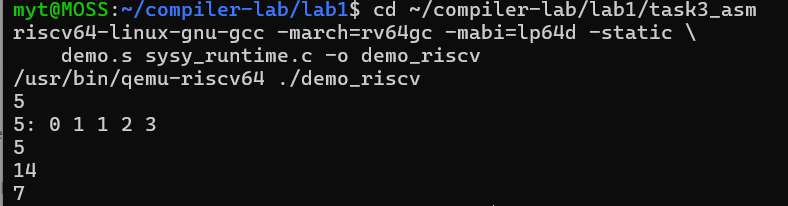
\includegraphics[width=0.92\textwidth]{task2_riscv/截图4.png}
  \caption{手写 demo.s 的交叉编译、静态链接与 QEMU 运行结果}
  \label{fig:riscv-build}
\end{figure}

程序运行结果如下：

\begin{lstlisting}
5
5: 0 1 1 2 3
5
14
7
\end{lstlisting}

逐行对照源程序检查输出，可以确认手写汇编被正确地翻译和执行了：

\begin{itemize}
  \item 第一行 5：putint(fib(5)) 的输出，$\mathrm{fib}(5)=5$。
  \item 第二行 5: 0 1 1 2 3：putarray(5, a) 的输出。数组 a 被第一个循环的前 5 次迭代分别赋以 x 的当前值。按斐波那契递推手算：第 0 轮时 x = 0，使 a[0] = 0；此后每轮 x 依次变为 1、1、2、3，故最终 $a=\{0,1,1,2,3\}$，与输出一致。
  \item 第三行 5：putint(sum) 的输出。在 $\{0,1,1,2,3\}$ 中，偶数元素直接累加、奇数元素累加 1，即 $0+1+1+2+1=5$，与输出一致。
  \item 第四行 14：putint(calc(7, 3)) 的输出，$(7+3)(7-3)/3+7\bmod 3 = 40/3+1 = 13+1 = 14$，与输出一致。
  \item 第五行 7：putint(calls) 的输出。fib 递归过程中，形参大于 1 的调用共发生 7 次（fib(5)、fib(4) 各一次，fib(3) 两次，fib(2) 三次），故 calls 为 7，与输出一致。
\end{itemize}

五项输出全部和人工推导一样，说明汇编程序实现了源程序的全部语义。

\noindent\textbf{交叉验证。}为进一步确认手写汇编与编译器理解一致，我还用交叉编译器对同一份 demo.c 生成了汇编（demo\_gcc.s），并对比两者的运行结果：

\begin{lstlisting}[language=bash]
cd ~/compiler-lab/lab1/task3_asm
riscv64-linux-gnu-gcc -S -march=rv64gc -mabi=lp64d -fno-stack-protector demo.c -o demo_gcc.s
riscv64-linux-gnu-gcc -march=rv64gc -mabi=lp64d -static demo_gcc.s sysy_runtime.c -o demo_gcc
/usr/bin/qemu-riscv64 ./demo_gcc
\end{lstlisting}

其输出与手写版本逐字节相同，说明二者的语义完全等价，对照如图~\ref{fig:riscv-cross} 所示。

\begin{figure}[H]
  \centering
  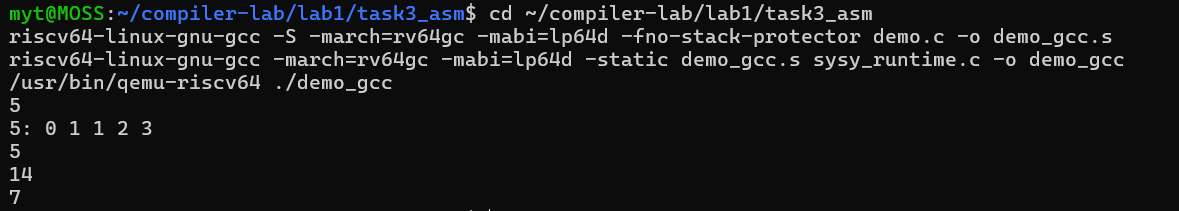
\includegraphics[width=0.92\textwidth]{task2_riscv/截图5.png}
  \caption{手写版 demo.s 与编译器生成版 demo\_gcc.s 的编译运行结果对照}
  \label{fig:riscv-cross}
\end{figure}

\subsubsection{思考}

\hfour{1、手写汇编与编译器生成代码的差异}

编译器在未优化（-O0）模式下会把每个局部变量都当作内存对象处理：i 改一次就 sw 回栈，下一步要用再 lw 出来，于是会出现大量写回—读出的往返；而手写版本把这些变量固定在 s 寄存器里，指令数明显更少。除此之外，编译器还会生成 .cfi\_startproc、.cfi\_def\_cfa\_offset 这类调试与异常展开指令，以及调用外部函数时带 @plt 的跳板形式。

\hfour{2、关于递归与寄存器保护}

编写 fib 时最深的体会是哪些寄存器需要压栈这件事，我最初就是先写了 mv a0,a0 这样想当然的代码，后来才意识到第二次 call fib 可能覆写 a0，必须先把结果转移到 s1 中，这让我理解了为什么跨函数调用存活的中间结果只能放在 s 寄存器这条规则必须严格遵守。

\hfour{3、关于 SysY 运行库的链接}

源程序用到的 putint、putch、putarray 不在标准库中，需要额外提供，所以在汇编编程的时候必须按调用约定传参，让被调函数能在 a0、a1 中拿到正确的实参。如果把参数顺序写反，或者忘了在调用前把数组首地址放入 a1，程序能正常链接，但运行结果会出错，这就是汇编编程与高级语言编程在编译期能查出多少错误上的根本差别：正确性只能靠自己对约定的准确把握。

\subsection{程序二：参数超过 8 个的函数}

\subsubsection{SysY 源程序}

RISC-V 提供了 a0–a7 八个参数寄存器，一旦函数的参数多于 8 个，多出来的那部分就必须由调用者放到栈上传递，我们设计的程序二专门用来考察这条边界。

manyargs.c 中有两个 10 参数的函数。mix 只做算术、不再调用他人；chain 也是 10 个参数，但它自己还要再调用一个 10 参数的 mix，所以从栈上接收自己的参数和为被调函数准备栈上的参数这两件事同时发生在同一个栈帧里。源程序如下：

\begin{lstlisting}[language=C]
#include "sysy.h"

int mix(int a, int b, int c, int d, int e, int f, int g, int h, int i, int j) {
    return (a - j) * (b - i) + (c - h) * (d - g) + e * f;
}

int chain(int a, int b, int c, int d, int e, int f, int g, int h, int i, int j) {
    return mix(j, i, h, g, f, e, d, c, b, a) + a * b + i * j;
}

int main() {
    putint(mix(1, 2, 3, 4, 5, 6, 7, 8, 9, 10));
    putch(10);
    putint(chain(1, 2, 3, 4, 5, 6, 7, 8, 9, 10));
    putch(10);

    int k = 0;
    int s = 0;
    while (k < 5) {
        s = s + mix(k, k + 1, k + 2, k + 3, k + 4, k + 5, k + 6, k + 7, k + 8, k + 9);
        k = k + 1;
    }
    putint(s);
    putch(10);

    return 0;
}
\end{lstlisting}

mix 的表达式 (a - j) * (b - i) + (c - h) * (d - g) + e * f 是故意这样排的：第 9、10 个参数 i、j 各自只出现一次，而且都参与减法，一旦取错了位置，结果立刻偏离。chain 故意把实参顺序整个倒过来传给 mix，逼着我们在汇编里处理一组寄存器之间的相互赋值。源程序截图如图~\ref{fig:riscv-manyargs-src} 所示。

\begin{figure}[H]
  \centering
  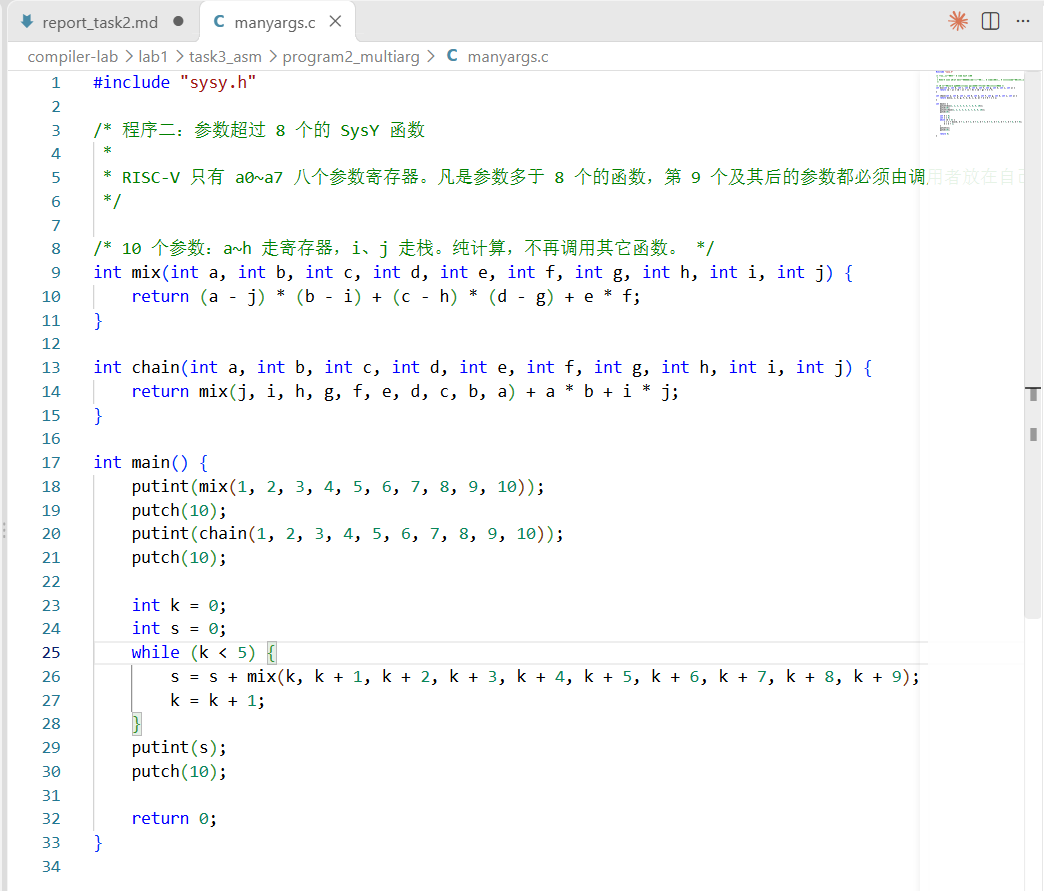
\includegraphics[width=0.78\textwidth]{task2_riscv/截图6.png}
  \caption{manyargs.c 源程序}
  \label{fig:riscv-manyargs-src}
\end{figure}

\subsubsection{汇编程序编写思路}

\hfour{1. 参数落位}

RV64 的整数参数依次使用 a0–a7；第 9 个及以后的参数，由调用者在调用点写入自己栈帧最低处的 0(sp)、8(sp)，每个槽占 8 字节，被调函数开辟自己的栈帧之后，再从 frame\_size(sp)、frame\_size+8(sp) 取回。mix 的栈帧是 16 字节，所以第 9 个参数 i 落在 16(sp)、第 10 个参数 j 落在 24(sp)，偏移量恰好等于栈帧大小。

\hfour{2. 栈帧的划分}

mix 用 16 字节，chain 用 64 字节，main 用 48 字节，都保持 16 字节对齐；chain 那 64 字节的最低 16 字节是留给调用 mix 的出参区，其余部分存放 ra、要跨调用保存的局部量，以及本函数自己的第 9、10 个参数。

\hfour{3. 寄存器分工}

mix 不调用任何函数；chain 和 main 都要发起调用，既要保存 ra，也要把用到的全部 s 寄存器压栈保护。跨调用还要用到的局部量一律放 s 寄存器——在 chain 里 i、j、a、b 在 call mix 返回后还要参与计算，而 t 寄存器是调用者保存的，mix 有权随意覆写。

\hfour{4. 关键语句的翻译策略}

\begin{itemize}
  \item \textbf{参数超过 8 个}：调用前先把第 9、10 个实参 sd 到 0(sp)、8(sp)；被调函数里用 lw 从 frame\_size 偏移处取回。调用者写的是完整的 8 字节槽，所以用 sd；被调函数只关心低 32 位，所以用 lw。
  \item \textbf{一组寄存器倒序赋值}：chain 要把 (j, i, h, g, f, e, d, c, b, a) 装进参数寄存器，其中 a2–a7 里本来是 (c, d, e, f, g, h)，需要倒过来写成 (h, g, f, e, d, c)。六个寄存器互相赋值必然彼此覆盖，所以先用 t0–t5 把六个值整体抄出来，再依次写回。
  \item \textbf{返回值直接接力}：mix 的返回值落在 a0，而 putint 也以 a0 接收实参。
\end{itemize}

依据上述思路，我最终编写出的汇编程序 manyargs.s 整体由表~\ref{tab:manyargscomp} 所示的几部分组成。

\begin{table}[H]
  \centering
  \small
  \setlength{\tabcolsep}{4pt}
  \begin{tabular}{>{\centering\arraybackslash}p{2.8cm}>{\centering\arraybackslash}p{6.4cm}>{\centering\arraybackslash}p{4.8cm}}
    \toprule
\headcol 部分 & \headcol 内容 & \headcol 对应源程序 \\
    \midrule
文件头 & 文件说明注释与汇编器指令 & — \\
    函数 mix & 10 参数的叶子函数，其中两个参数取自栈 & int mix(...) \\
    函数 chain & 10 参数，且自己再调用 mix & int chain(...) \\
    函数 main & 常数调用、嵌套调用与循环调用 & int main() \\
    收尾标识 & .ident 与栈属性标记 & — \\
    \bottomrule
\end{tabular}
  \caption{手写汇编程序 manyargs.s 的组成}
  \label{tab:manyargscomp}
\end{table}

manyargs.s 的全文整体缩略视图如图~\ref{fig:riscv-manyargs-s} 所示。

\begin{figure}[H]
  \centering
  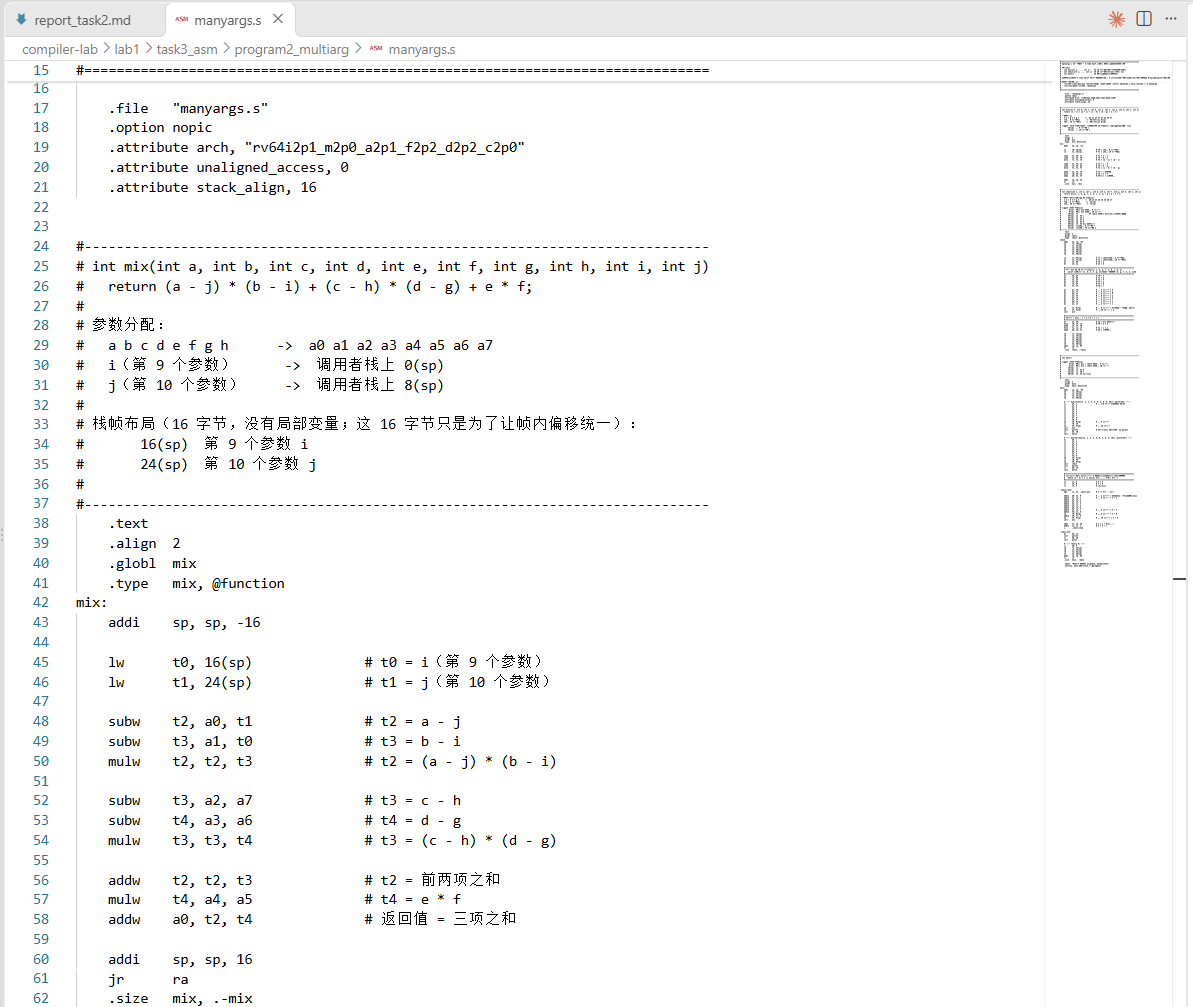
\includegraphics[width=0.92\textwidth]{task2_riscv/截图7.png}
  \caption{手写汇编程序 manyargs.s 全文（编辑器整体缩略视图）}
  \label{fig:riscv-manyargs-s}
\end{figure}

\subsubsection{汇编程序分析}

文件头与收尾标识部分与程序一完全相同，此处不再重复。下面重点分析三个函数。

\hfour{1. 函数 mix}

\begin{lstlisting}[language=riscv]
    .text
    .align  2
    .globl  mix
    .type   mix, @function
mix:
    addi    sp, sp, -16

    lw      t0, 16(sp)              # t0 = i（第 9 个参数）
    lw      t1, 24(sp)              # t1 = j（第 10 个参数）

    subw    t2, a0, t1              # t2 = a - j
    subw    t3, a1, t0              # t3 = b - i
    mulw    t2, t2, t3              # t2 = (a - j) * (b - i)

    subw    t3, a2, a7              # t3 = c - h
    subw    t4, a3, a6              # t4 = d - g
    mulw    t3, t3, t4              # t3 = (c - h) * (d - g)

    addw    t2, t2, t3              # t2 = 前两项之和
    mulw    t4, a4, a5              # t4 = e * f
    addw    a0, t2, t4              # 返回值 = 三项之和

    addi    sp, sp, 16
    jr      ra
\end{lstlisting}

前八个参数 a–h 由 a0–a7 直接传入，第 9、10 个参数 i、j 则在 16(sp)、24(sp)。这两个偏移等于调用者写下的 0(sp)、8(sp) 再加上本函数自己下移的 16 字节，也就是栈帧大小。

计算部分与程序一中的 calc 是一套手法：用带 w 后缀的 subw、mulw、addw 按 32 位运算并自动符号扩展，与 C 语言中 int 的语义对应。把数组式的参数表映射到寄存器上之后有个好处：(c - h)、(d - g) 这些项可以直接在 a 寄存器之间做减法，不用先搬到临时寄存器。mix 不调用任何其它函数，因此既不需要保存 ra，也不需要动用任何 s 寄存器。

\hfour{2. 函数 chain}

\textbf{（1）入口、栈帧与入参取回。}

\begin{lstlisting}[language=riscv]
chain:
    addi    sp, sp, -64
    sd      ra, 16(sp)
    sd      s1, 24(sp)
    sd      s2, 32(sp)
    sd      s3, 40(sp)
    sd      s4, 48(sp)
    sd      s5, 56(sp)

    lw      s1, 64(sp)              # s1 = i（自己的第 9 个参数）
    lw      s2, 72(sp)              # s2 = j（自己的第 10 个参数）
    mv      s3, a0                  # s3 = a
    mv      s4, a1                  # s4 = b
\end{lstlisting}

chain 的栈帧是 64 字节，所以它自己的第 9、10 个参数落在 64(sp)、72(sp)。栈帧内部布局如下：

\begin{lstlisting}
    sp + 0   ... sp + 15    调用 mix 时的出参区（第 9、10 个实参）
    sp + 16                ra
    sp + 24                s1  —— i
    sp + 32                s2  —— j
    sp + 40                s3  —— a
    sp + 48                s4  —— b
    sp + 56                s5  —— mix 的返回值
    sp + 64                本函数自己的第 9 个参数 i
    sp + 72                本函数自己的第 10 个参数 j
\end{lstlisting}

这里同时存在两个第 9 个参数：64(sp) 处是别人传给 chain 的，0(sp) 处是 chain 准备传给 mix 的。之所以 i、j 取回后立刻转存到 s1、s2，是因为下面要调用 mix。

\textbf{（2）准备 mix 的十个实参。}

\begin{lstlisting}[language=riscv]
    mv      t0, a7                  # t0 = h
    mv      t1, a6                  # t1 = g
    mv      t2, a5                  # t2 = f
    mv      t3, a4                  # t3 = e
    mv      t4, a3                  # t4 = d
    mv      t5, a2                  # t5 = c

    mv      a2, t0                  # 第 3 个实参 = h
    mv      a3, t1                  # 第 4 个实参 = g
    mv      a4, t2                  # 第 5 个实参 = f
    mv      a5, t3                  # 第 6 个实参 = e
    mv      a6, t4                  # 第 7 个实参 = d
    mv      a7, t5                  # 第 8 个实参 = c
    mv      a0, s2                  # 第 1 个实参 = j
    mv      a1, s1                  # 第 2 个实参 = i

    sd      s4, 0(sp)               # 第 9 个实参 = b，写到出参区最低两个槽
    sd      s3, 8(sp)               # 第 10 个实参 = a
    call    mix
\end{lstlisting}

实参表 mix(j, i, h, g, f, e, d, c, b, a) 相对于形参表是倒序的。前两个实参来自 s2、s1，不会冲突；a2–a7 内部是一个六元置换，如果直接按顺序写 mv a2,a7、mv a3,a6 …… 那么写完 a2 时原来的 a2 就没了，而后面还要用它，因此先把六个值整体抄到 t0–t5，再依次写回，这就是那些 mv 存在的原因。最后两行把 b、a 写到出参区。

\textbf{（3）返回值的组装。}

\begin{lstlisting}[language=riscv]
    mv      s5, a0                  # s5 = mix 的返回值
    mulw    t0, s3, s4              # t0 = a * b
    addw    s5, s5, t0
    mulw    t1, s1, s2              # t1 = i * j
    addw    a0, s5, t1              # a0 = 三项之和
\end{lstlisting}

call mix 返回后，a0 中是 mix 的结果。因为 mix 只写 a 和 t 寄存器、不会碰 s 寄存器，所以 s1–s4 里的 i、j、a、b 依然可用，可以直接拿来算 a * b 和 i * j。

\hfour{3. 函数 main}

\textbf{（1）栈帧与常数调用。}

\begin{lstlisting}[language=riscv]
main:
    addi    sp, sp, -48
    sd      ra, 16(sp)
    sd      s1, 24(sp)
    sd      s2, 32(sp)
    sd      s3, 40(sp)

    li      a0, 1                   # 第 1~8 个实参依次装入 a0~a7
    li      a1, 2
    li      a2, 3
    li      a3, 4
    li      a4, 5
    li      a5, 6
    li      a6, 7
    li      a7, 8
    li      t0, 9
    sd      t0, 0(sp)               # 第 9 个实参
    li      t0, 10
    sd      t0, 8(sp)               # 第 10 个实参
    call    mix
    call    putint                  # 返回值已在 a0，直接传给 putint
\end{lstlisting}

48 字节的栈帧里，最低的 16 字节是出参区，其余留给 ra 和三个 s 寄存器。布置实参时前八个直接 li 进 a0–a7，后两个先 li 到临时寄存器再 sd 进栈。

\textbf{（2）循环中的重复布置。}

\begin{lstlisting}[language=riscv]
    li      s1, 0                   # k = 0
    li      s2, 0                   # s = 0
    li      s3, 5                   # 循环上界

.Lmain_loop:
    bge     s1, s3, .Lmain_out      # k >= 5，退出循环

    addiw   a0, s1, 0               # 第 1 个实参 = k（addiw 顺带做符号扩展）
    addiw   a1, s1, 1               # 第 2 个实参 = k + 1
    addiw   a2, s1, 2
    addiw   a3, s1, 3
    addiw   a4, s1, 4
    addiw   a5, s1, 5
    addiw   a6, s1, 6
    addiw   a7, s1, 7               # 第 8 个实参 = k + 7
    addiw   t0, s1, 8
    sd      t0, 0(sp)               # 第 9 个实参 = k + 8
    addiw   t0, s1, 9
    sd      t0, 8(sp)               # 第 10 个实参 = k + 9
    call    mix

    addw    s2, s2, a0              # s = s + mix(...)
    addiw   s1, s1, 1               # k = k + 1
    j       .Lmain_loop
\end{lstlisting}

这里用 addiw 来构造实参，是因为 k 是 32 位的 int，addiw 在做加法之余会把结果符号扩展成 64 位。循环每次都要重新往 a0–a7 和 0(sp)、8(sp) 里填一遍。

\hfour{4. 函数返回与文件结尾}

\begin{lstlisting}[language=riscv]
.Lmain_out:
    mv      a0, s2
    call    putint
    li      a0, 10
    call    putch

    li      a0, 0
    ld      ra, 16(sp)
    ld      s1, 24(sp)
    ld      s2, 32(sp)
    ld      s3, 40(sp)
    addi    sp, sp, 48
    jr      ra
\end{lstlisting}

恢复顺序与入口严格相反，addi sp, sp, 48 收回栈帧后 jr ra 返回。收尾的 .ident 与 .section .note.GNU-stack 和程序一相同。

\subsubsection{编译与验证}

验证流程与程序一完全一致，只是换到程序二自己的目录：

\begin{lstlisting}[language=bash]
cd ~/compiler-lab/lab1/task3_asm/program2_multiarg
riscv64-linux-gnu-gcc -march=rv64gc -mabi=lp64d -static \
    manyargs.s sysy_runtime.c -o manyargs
/usr/bin/qemu-riscv64 ./manyargs
\end{lstlisting}

编译与运行的终端回显如图~\ref{fig:riscv-manyargs-build} 所示。

\begin{figure}[H]
  \centering
  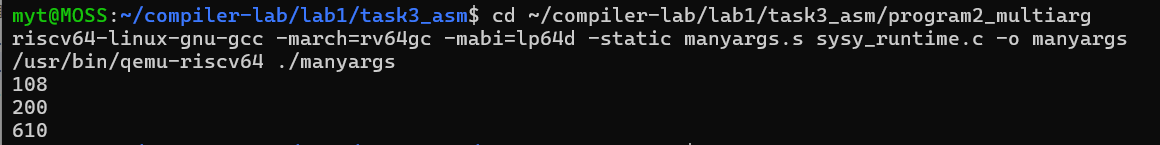
\includegraphics[width=0.92\textwidth]{task2_riscv/截图8.png}
  \caption{手写 manyargs.s 的交叉编译、静态链接与 QEMU 运行结果}
  \label{fig:riscv-manyargs-build}
\end{figure}

程序运行结果如下：

\begin{lstlisting}
108
200
610
\end{lstlisting}

逐项对照源程序检查：

\begin{itemize}
  \item 第一行 108：putint(mix(1, 2, 3, 4, 5, 6, 7, 8, 9, 10)) 的输出。代入 $a=1,\ldots,j=10$，得 $(1-10)(2-9)$ $+(3-8)(4-7)$ $+5\times 6$ $= 63+15+30$ $= 108$，与输出一致。
  \item 第二行 200：putint(chain(1, 2, 3, 4, 5, 6, 7, 8, 9, 10)) 的输出。先算内层 $\mathrm{mix}(10,9,8,7,6,5,4,3,2,1)=108$，再加上 $a\times b+i\times j$ $=1\times 2+9\times 10$ $=92$，合计 $108+92=200$，与输出一致。
  \item 第三行 610：循环中五次 mix(k, k+1, …, k+9) 的累加。把表达式化简后每一项为 $98+k^2+9k$，$k=0\ldots 4$ 时依次是 98、108、120、134、150，总和为 $98+108$ $+120+134+150$ $=610$，与输出一致。
\end{itemize}

三项输出全部与人工推导一样。

同样用交叉编译器从 manyargs.c 生成一份汇编，比较两者的运行结果：

\begin{lstlisting}[language=bash]
cd ~/compiler-lab/lab1/task3_asm/program2_multiarg
riscv64-linux-gnu-gcc -S -march=rv64gc -mabi=lp64d -fno-stack-protector manyargs.c -o manyargs_gcc.s
riscv64-linux-gnu-gcc -march=rv64gc -mabi=lp64d -static manyargs_gcc.s sysy_runtime.c -o manyargs_gcc
/usr/bin/qemu-riscv64 ./manyargs_gcc
\end{lstlisting}

输出与手写版本相同，对比如图~\ref{fig:riscv-manyargs-cross} 所示。编译器生成的版本也在做同一件事：它的 mix 以 s0 作为帧指针，读第 9、10 个参数用的是 0(s0)、8(s0)，即 sp 加栈帧大小，与我们手写版取的 16(sp)、24(sp) 是同一条规则；调用点同样是把实参 sd 到 0(sp)、8(sp)，说明我们对调用约定的理解与编译器是一致的。

\begin{figure}[H]
  \centering
  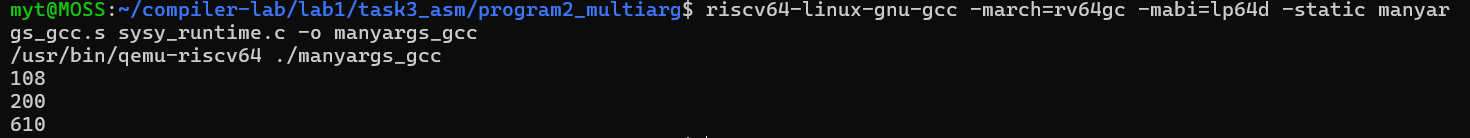
\includegraphics[width=0.92\textwidth]{task2_riscv/截图9.png}
  \caption{手写版 manyargs.s 与编译器生成版 manyargs\_gcc.s 的运行结果对照}
  \label{fig:riscv-manyargs-cross}
\end{figure}

\subsubsection{思考}

\hfour{1、关于 8 这个边界}

在写程序二时我才意识到，a0–a7 只有八个，超过八个就必须在栈上留位置、在调用前后手动搬进搬出。并且偏移等于栈帧大小意味着：被调函数取栈上参数的偏移，取决于它自己开了多大的栈帧，而不是一个固定值。

\hfour{2、关于两个第 9 个参数}

chain 里最绕的地方，是同一个函数里同时出现了别人给我的第 9 个参数和我给 mix 的第 9 个参数，分别在 64(sp) 和 0(sp)。如果栈帧没算对，比如漏算了出参区那 16 字节，两个位置就会错位、甚至互相覆盖，这类错误不会报错、不会崩溃，只会让结果偏掉。

\hfour{3、关于一组寄存器的相互赋值}

chain 里把 (c,d,e,f,g,h) 倒成 (h,g,f,e,d,c) 的那六个 mv 拷贝，让我知道寄存器是会被覆盖的稀缺资源：凡是一个值还要用、而目标位置已经被占的场合，都得先腾出地方。高级语言里这一层被编译器完全接管了，只有自己写汇编才会面对它。

\section{进阶要求：观察 AI 编译器 MLIR 的中端处理过程}

本章为进阶要求部分，主题是\textbf{观察 AI 编译器 MLIR 的中端（middle-end）处理过程}：亲手编写一个贴近 AI 负载的 MLIR 样例（矩阵乘 + 偏置 + ReLU），用 mlir-opt-18 让它依次流经从高层 linalg 方言到 LLVM 方言的完整流水线，逐阶段转储真实的 IR，把“中端处理”这一平时不可见的黑盒打开来看。所用的 MLIR 18.1.3 环境版本信息已在第一章给出（见图~\ref{fig:envversions}）。

\subsection{实验原理}

\subsubsection{为什么 AI 编译器需要“多级”中间表示}

传统编译器（如 GCC、Clang）大多只有\textbf{一层}中间表示：源码先降到它，优化都在它上面做，最后再降到机器码。但 AI 编译器面对的场景要复杂得多：

\begin{itemize}
  \item \textbf{算子层次高。} 神经网络的计算是“矩阵乘”“卷积”“归一化”这类\textbf{领域算子}，它们天然是粗粒度的循环嵌套，若一开始就拆成标量加减乘除，后续的融合、切分、向量化就无从谈起。
  \item \textbf{硬件后端多。} 同一段模型可能要跑在 CPU、GPU、NPU、DSP 上，不同硬件的内存层次、并行方式差异极大。
  \item \textbf{优化发生在多个层次。} 算子融合、循环分块（tiling）发生在高层；向量化、寄存器分配发生在低层。\textbf{每一层都有自己适用的优化}，用同一层 IR 硬做所有优化既别扭又低效。
\end{itemize}

于是就有了 MLIR（Multi-Level Intermediate Representation）的基本主张：\textbf{不要一层 IR 包打天下，而要让 IR 分层次地存在}。程序以“高层方言”入场，沿着一串处理趟逐步下降到“低层方言”，最终落到可直接生成机器码的 LLVM 方言。这一过程称为\textbf{渐进式下降（progressive lowering）}，而这一路上的每一步，正是“中端处理”。

\subsubsection{MLIR 的三个核心抽象}

\begin{table}[H]
  \centering
  \small
  \setlength{\tabcolsep}{4pt}
  \begin{tabular}{>{\centering\arraybackslash}p{1.8cm}>{\centering\arraybackslash}p{2.2cm}>{\centering\arraybackslash}p{10.6cm}}
    \toprule
\headcol 抽象 & \headcol 英文 & \headcol 含义 \\
    \midrule
操作 & Operation & MLIR 中的\textbf{一切}都是操作：运算、函数、循环、甚至模块本身。它是唯一的通用 IR 单位。 \\
    方言 & Dialect & 一组操作的\textbf{集合与命名空间}，代表一个抽象层级或一个领域。如 arith（算术）、linalg（线性代数）、scf（结构化控制流）、cf（控制流图）、llvm（LLVM 对接层）。 \\
    处理趟 & Pass & 一次\textbf{遍（pass）}：以操作树为单位做一次变换或分析。多个趟串起来就是\textbf{趟流水线（Pass Pipeline）}。 \\
    \bottomrule
\end{tabular}
  \caption{MLIR 的三个核心抽象}
  \label{tab:mlirabstract}
\end{table}

三者关系可以概括为：\textbf{IR 是一棵由 Operation 组成的树，每个 Operation 归属某个 Dialect，Pass 负责把这棵树从一种方言形态改写成另一种形态。}与之配套的还有两个概念：

\begin{itemize}
  \item \textbf{属性（Attribute）}与\textbf{类型（Type）}：方言可以自定义自己的属性与类型；
  \item \textbf{接口（Interface）}：方言可以声明自己如何被转换到其他方言（如 linalg 声明“我能降到循环”），于是通用的 --convert-to-llvm 就能自动找到合适的下降路径。
\end{itemize}

\subsubsection{从 linalg 到 LLVM 的下降路线}

本实验采用一条经典且完整的下降路线，如代码~\ref{code:lowering} 所示。

\begin{lstlisting}[label=code:lowering]
linalg.matmul（具名算子）
   |  --linalg-generalize-named-ops      泛化为通用算子 linalg.generic
   v
linalg.generic
   |  --convert-linalg-to-affine-loops   降为 affine 循环嵌套（多面体表示）
   v
affine.for / affine.load / affine.store
   |  --lower-affine                     降为 scf.for + arith + memref
   v
scf.for（结构化控制流）
   |  --convert-scf-to-cf                结构化控制流降为基本块 CFG
   v
cf.br / cf.cond_br（控制流图）
   |  --convert-to-llvm + --reconcile-unrealized-casts
   v
llvm.*（LLVM 方言）
   |  mlir-translate-18 --mlir-to-llvmir
   v
LLVM IR（.ll）
\end{lstlisting}

每一层的 IR 都\textbf{仍然是一个完整、自洽、可独立验证的程序}，这正是“多级表示”的精髓：可以在任意一级停下来观察、改写、再继续。这也是它与“一次翻译到底”的传统中间代码生成最本质的区别。

\subsubsection{观察中端处理的手段}

MLIR 把“观察”做成了工具的内建能力——mlir-opt 提供了一组打印选项，可以在\textbf{不做任何手工插桩}的情况下把每一步的 IR 转储出来，如表~\ref{tab:mliroptions} 所示。

\begin{table}[H]
  \centering
  \small
  \setlength{\tabcolsep}{4pt}
  \begin{tabular}{>{\centering\arraybackslash}p{4.8cm}>{\centering\arraybackslash}p{9.8cm}}
    \toprule
\headcol 选项 & \headcol 作用 \\
    \midrule
--mlir-print-ir-before-all & 每个 pass \textbf{执行前}打印一份 IR \\
    --mlir-print-ir-after-all & 每个 pass \textbf{执行后}打印一份 IR（最常用） \\
    --mlir-print-ir-after-change & 仅当该 pass \textbf{确实改动了} IR 时才打印 \\
    --mlir-print-ir-module-scope & 始终以整个模块为粒度打印（默认按最近的 IsolatedFromAbove 操作打印） \\
    --mlir-print-op-generic & 用通用语法打印，便于看清操作的真实参数结构 \\
    --mlir-disable-threading & 关闭多线程，保证打印顺序稳定、可复现 \\
    \bottomrule
\end{tabular}
  \caption{mlir-opt 常用的 IR 打印选项}
  \label{tab:mliroptions}
\end{table}

配合 mlir-translate-18 --mlir-to-llvmir，就能把流水线的终点接到 LLVM 后端，从而把“AI 编译器”与“经典编译器”这两套体系对接起来观察。

\subsection{实验步骤与结果}

\subsubsection{样例程序：一个贴近 AI 负载的 gemm.mlir}

为了让观察对象具有“AI 编译器”的味道，样例不写成普通的算术程序，而写成一个典型的神经网络小负载——\textbf{矩阵乘 + 偏置 + ReLU}：

$$C = \mathrm{relu}(A \times B + \mathrm{bias})$$

其中 $A$ 为 $4\times8$、$B$ 为 $8\times4$、结果 $C$ 为 $4\times4$。程序清单如下（gemm.mlir，共 31 行）：

\begin{lstlisting}[language=MLIR]
// gemm.mlir —— 一个典型的“AI 负载”：矩阵乘 + 偏置 + ReLU
// C = relu(A * B + bias)
// 使用 MLIR 的高层方言 linalg / arith / memref / func 书写。

module {
  func.func @matmul_bias_relu(%A: memref<4x8xf32>,
                              %B: memref<8x4xf32>,
                              %bias: memref<4xf32>,
                              %C: memref<4x4xf32>) {
    %cst = arith.constant 0.0 : f32

    // 第一步：C = A * B
    linalg.fill ins(%cst : f32) outs(%C : memref<4x4xf32>)
    linalg.matmul ins(%A, %B : memref<4x8xf32>, memref<8x4xf32>)
                  outs(%C : memref<4x4xf32>)

    // 第二步：C = relu(C + bias[j])
    linalg.generic {
        indexing_maps = [affine_map<(i, j) -> (i, j)>,
                         affine_map<(i, j) -> (j)>,
                         affine_map<(i, j) -> (i, j)>],
        iterator_types = ["parallel", "parallel"]}
      ins(%C, %bias : memref<4x4xf32>, memref<4xf32>)
      outs(%C : memref<4x4xf32>) {
      ^bb0(%c: f32, %b: f32, %o: f32):
        %s = arith.addf %c, %b : f32
        %r = arith.maximumf %s, %cst : f32
        linalg.yield %r : f32
    }
    return
  }
}
\end{lstlisting}

gemm.mlir 的全部内容如图~\ref{fig:mlir-gemm} 所示。这份样例值得说明的地方有三点：

\begin{figure}[H]
  \centering
  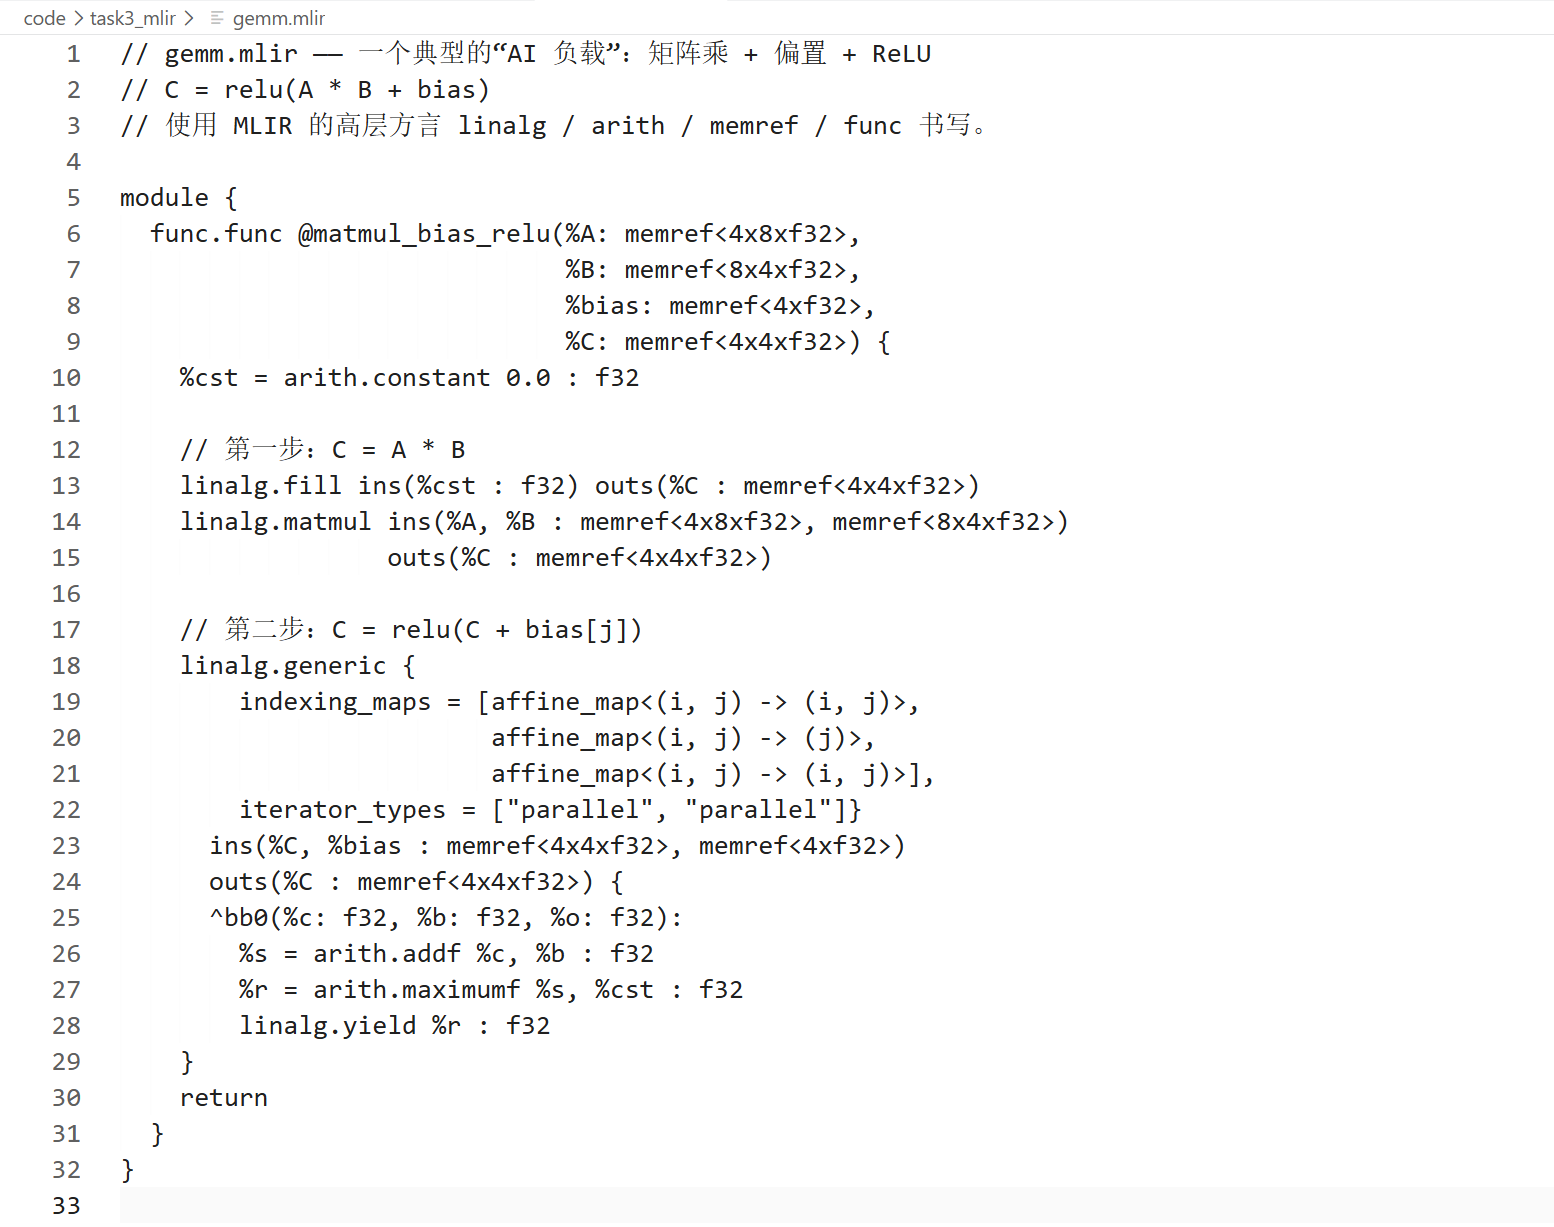
\includegraphics[width=0.85\textwidth]{advanced/2.png}
  \caption{gemm.mlir 的全部内容（高层 linalg 方言书写的 AI 负载）}
  \label{fig:mlir-gemm}
\end{figure}

\begin{itemize}
  \item \textbf{其一}，linalg 是 MLIR 中承载“线性代数/张量计算”的高层方言，linalg.matmul 是一个\textbf{具名算子（named op）}，它把“矩阵乘”作为一个整体概念来表达，而不是三个嵌套循环——这正是 AI 编译器关心的粒度。
  \item \textbf{其二}，indexing\_maps 用仿射映射描述“循环下标 $\to$ 数组下标”的关系，iterator\_types 标注每个循环维是 parallel 还是 reduction。\textbf{这是从高层算子自动导出循环结构的依据}，也是后面能自动生成循环的直接原因。
  \item \textbf{其三}，样例使用的是 memref（已分配的内存缓冲区）而非 tensor，因此跳过了 bufferization（张量到缓冲的转换）这一步，让观察聚焦在“循环与方言下降”本身。
\end{itemize}

\subsubsection{逐阶段的渐进式下降}

下面的每个阶段都用 mlir-opt-18 单独导出一次 IR。

\hfour{1、阶段零：确认输入可解析}

\begin{lstlisting}[language=bash]
mlir-opt-18 gemm.mlir
\end{lstlisting}

mlir-opt 不指定任何 --pass 时，只做解析与打印（并顺带做规范化输出）。能原样回显，说明样例语法正确，回显结果如图~\ref{fig:mlir-00} 所示。

\begin{figure}[H]
  \centering
  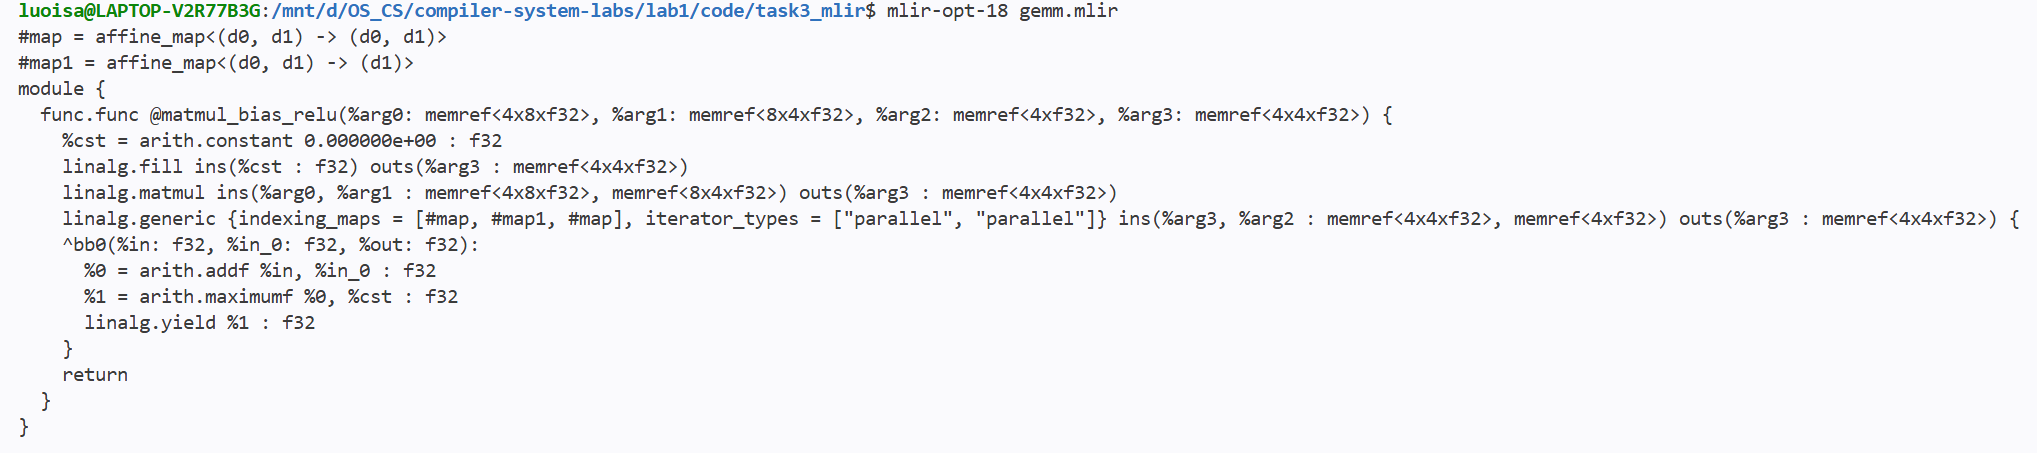
\includegraphics[width=0.92\textwidth]{advanced/01.png}
  \caption{mlir-opt-18 无 pass 回显 gemm.mlir，输入可正常解析}
  \label{fig:mlir-00}
\end{figure}

\hfour{2、阶段一：具名算子泛化为 linalg.generic}

\begin{lstlisting}[language=bash]
mlir-opt-18 gemm.mlir --linalg-generalize-named-ops
\end{lstlisting}

--linalg-generalize-named-ops 把 linalg.fill、linalg.matmul 这类“具名算子”统一改写为它们的“通用形式” linalg.generic，输出如图~\ref{fig:mlir-01} 所示。改写后，原本一句话的 linalg.matmul 被明确展开为带 arith.mulf / arith.addf 的循环体（真实输出，节选）：

\begin{lstlisting}[language=MLIR]
    linalg.generic {indexing_maps = [#map2, #map3, #map4], iterator_types = ["parallel", "parallel", "reduction"]} ins(%arg0, %arg1 : memref<4x8xf32>, memref<8x4xf32>) outs(%arg3 : memref<4x4xf32>) {
    ^bb0(%in: f32, %in_0: f32, %out: f32):
      %0 = arith.mulf %in, %in_0 : f32
      %1 = arith.addf %out, %0 : f32
      linalg.yield %1 : f32
    }
\end{lstlisting}

\begin{figure}[H]
  \centering
  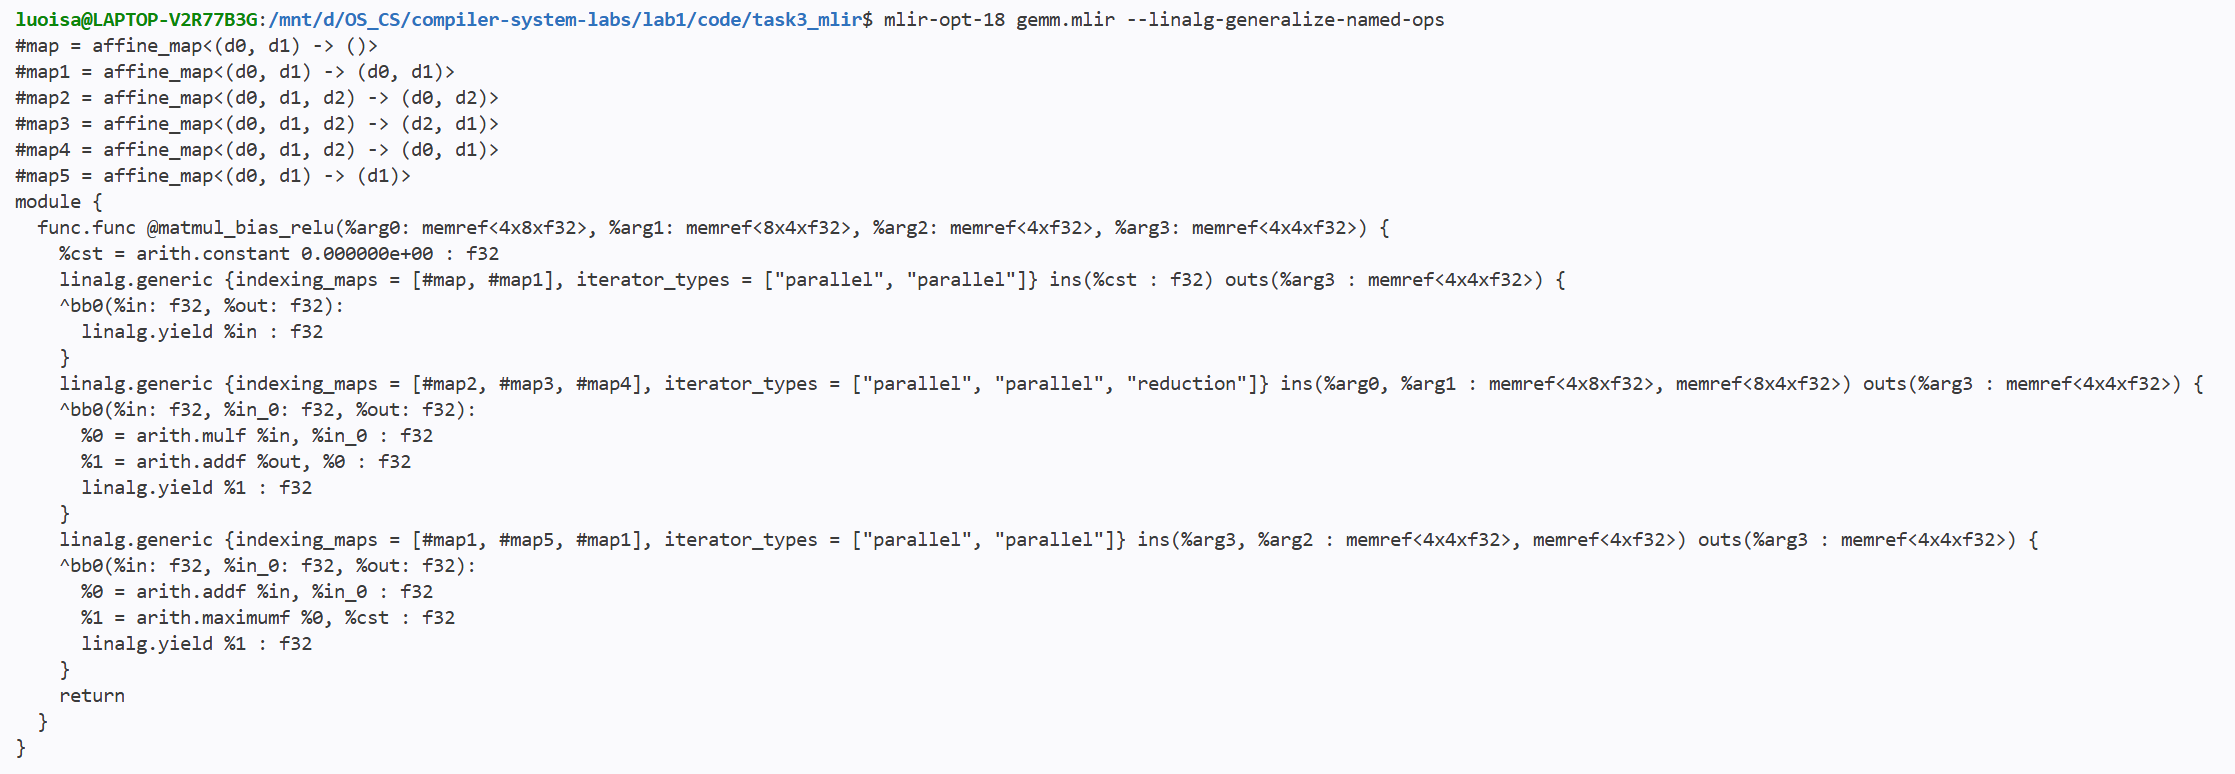
\includegraphics[width=0.92\textwidth]{advanced/02.png}
  \caption{具名算子被泛化为 linalg.generic，并行/归约维被显式标注}
  \label{fig:mlir-01}
\end{figure}

值得注意的是，输出里出现了 iterator\_types = [“parallel”, “parallel”, “reduction”]——第三个 reduction 维度正是矩阵乘在 $k$ 方向上的\textbf{归约}（累加）维。\textbf{同一个具名算子，其“并行/归约”的结构被显式地摆到了台面上}，这正是高层算子向下下降时最关键的信息。

\hfour{3、阶段二：linalg 下降为 affine 循环嵌套}

\begin{lstlisting}[language=bash]
mlir-opt-18 gemm.mlir \
  --linalg-generalize-named-ops \
  --convert-linalg-to-affine-loops
\end{lstlisting}

--convert-linalg-to-affine-loops 依据上一步的 indexing\_maps 与 iterator\_types，\textbf{自动生成}仿射循环嵌套，输出如图~\ref{fig:mlir-02} 所示。原来的 linalg.matmul 此刻已经变成教科书里的三重循环（真实输出，节选）：

\begin{lstlisting}[language=MLIR]
    affine.for %arg4 = 0 to 4 {
      affine.for %arg5 = 0 to 4 {
        affine.for %arg6 = 0 to 8 {
          %0 = affine.load %arg0[%arg4, %arg6] : memref<4x8xf32>
          %1 = affine.load %arg1[%arg6, %arg5] : memref<8x4xf32>
          %2 = affine.load %arg3[%arg4, %arg5] : memref<4x4xf32>
          %3 = arith.mulf %0, %1 : f32
          %4 = arith.addf %2, %3 : f32
          affine.store %4, %arg3[%arg4, %arg5] : memref<4x4xf32>
        }
      }
    }
\end{lstlisting}

\begin{figure}[H]
  \centering
  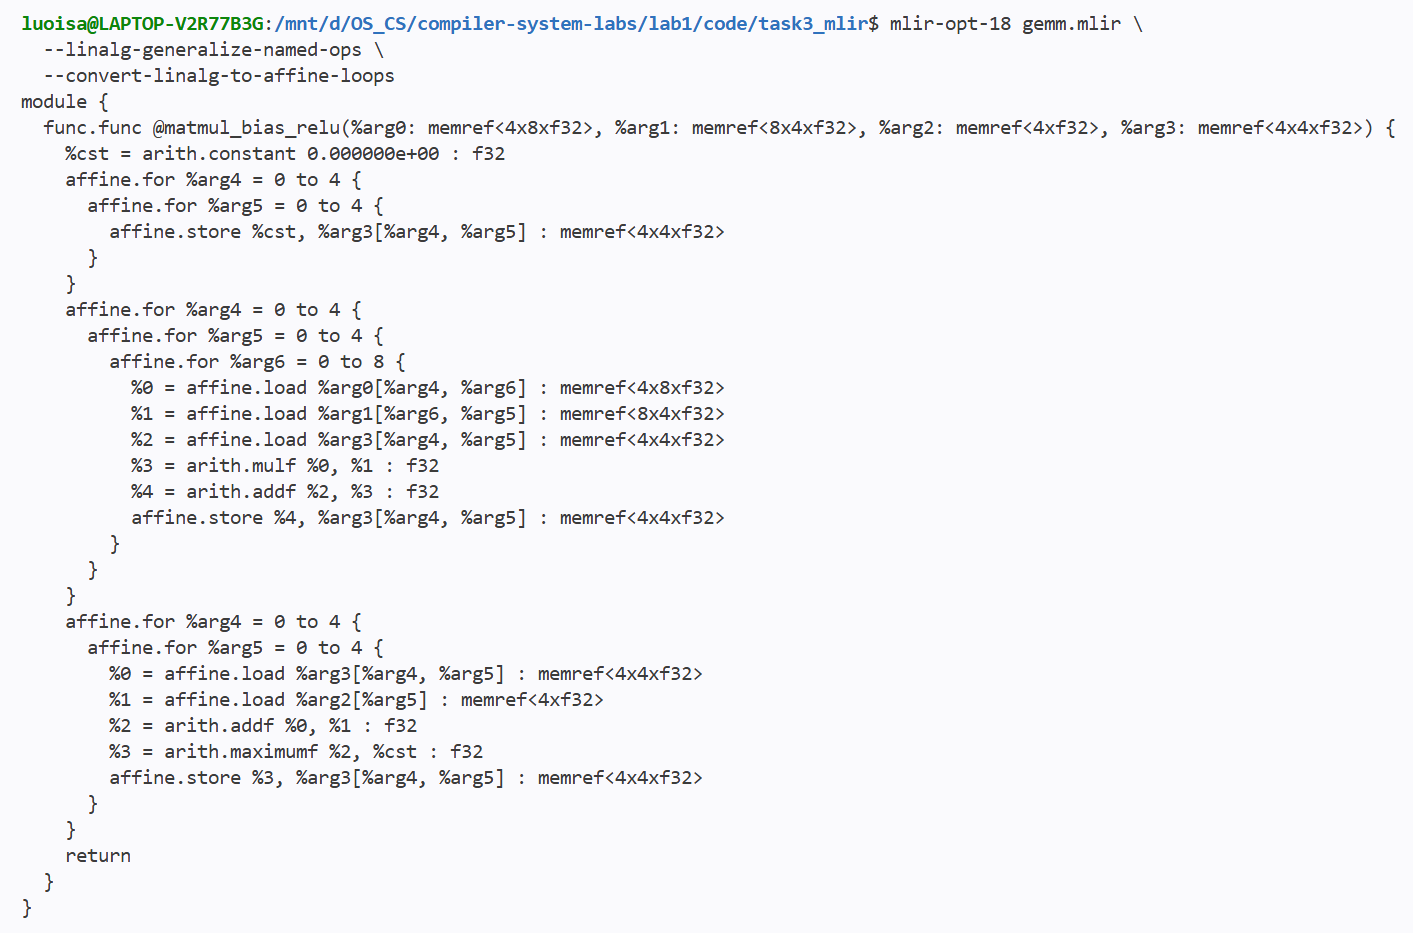
\includegraphics[width=0.92\textwidth]{advanced/03.png}
  \caption{linalg 算子被自动改写为三重 affine.for 循环嵌套}
  \label{fig:mlir-02}
\end{figure}

这里的 affine 方言是\textbf{多面体（polyhedral）优化}的载体：循环边界与下标都是仿射表达式（$i$、$j$、$k$ 的线性组合），因此可以做循环分块、交换、倾斜等变换。AI 编译器里常说的“算子融合”“循环切分”大多就发生在这一层或其等价层。

\hfour{4、阶段三：affine 下降为 scf（结构化控制流）}

\begin{lstlisting}[language=bash]
mlir-opt-18 gemm.mlir \
  --linalg-generalize-named-ops \
  --convert-linalg-to-affine-loops \
  --lower-affine
\end{lstlisting}

--lower-affine 把仿射层的“舒适写法”还原为更通用的形式：affine.for 变为 scf.for，affine.load/affine.store 变为 memref.load/memref.store，输出如图~\ref{fig:mlir-03} 所示。真实输出（节选）：

\begin{lstlisting}[language=MLIR]
    %c0_0 = arith.constant 0 : index
    %c4_1 = arith.constant 4 : index
    %c1_2 = arith.constant 1 : index
    scf.for %arg4 = %c0_0 to %c4_1 step %c1_2 {
      %c0_6 = arith.constant 0 : index
      %c4_7 = arith.constant 4 : index
      %c1_8 = arith.constant 1 : index
      scf.for %arg5 = %c0_6 to %c4_7 step %c1_8 {
        %c0_9 = arith.constant 0 : index
        %c8 = arith.constant 8 : index
        %c1_10 = arith.constant 1 : index
        scf.for %arg6 = %c0_9 to %c8 step %c1_10 {
          %0 = memref.load %arg0[%arg4, %arg6] : memref<4x8xf32>
          %1 = memref.load %arg1[%arg6, %arg5] : memref<8x4xf32>
          %2 = memref.load %arg3[%arg4, %arg5] : memref<4x4xf32>
          %3 = arith.mulf %0, %1 : f32
          %4 = arith.addf %2, %3 : f32
          memref.store %4, %arg3[%arg4, %arg5] : memref<4x4xf32>
        }
      }
    }
\end{lstlisting}

\begin{figure}[H]
  \centering
  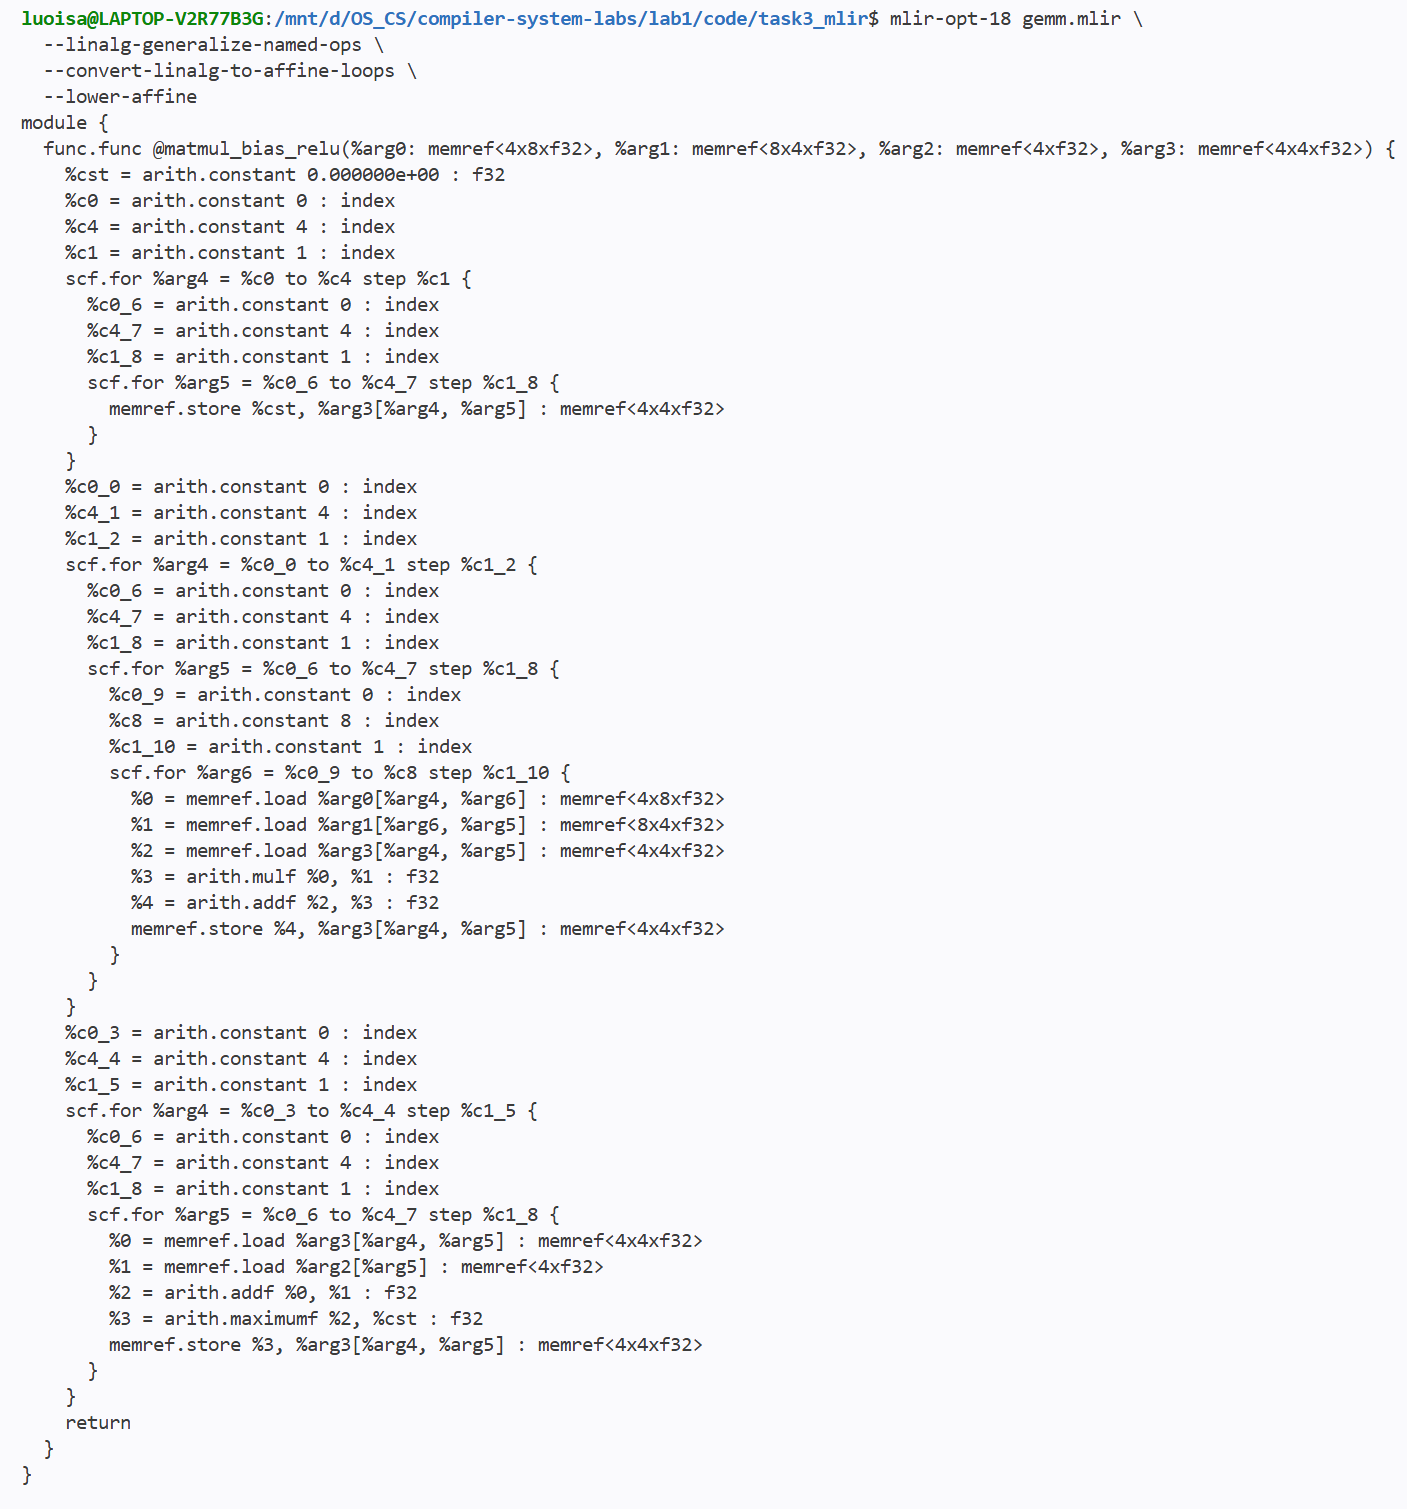
\includegraphics[width=0.92\textwidth]{advanced/04.png}
  \caption{affine 循环被下降为 scf.for 与 memref.load/store}
  \label{fig:mlir-03}
\end{figure}

此时循环仍是\textbf{结构化}的（scf.for 有明确的起止与步长），循环变量是 index 类型，下标访问退化为 memref.load/store。可以注意到一个细节：affine 层用 \%argN 变量隐式表示循环变量，而 scf 层显式地把上下界与步长都写成了 arith.constant——\textbf{同一语义，表示精度不同}，这正是“多级”的直观体现。

\hfour{5、阶段四：scf 下降为 cf（基本块 CFG）}

\begin{lstlisting}[language=bash]
mlir-opt-18 gemm.mlir \
  --linalg-generalize-named-ops \
  --convert-linalg-to-affine-loops \
  --lower-affine \
  --convert-scf-to-cf
\end{lstlisting}

--convert-scf-to-cf 把结构化循环“摊平”成\textbf{基本块 + 条件/无条件跳转}，即控制流图（CFG），输出如图~\ref{fig:mlir-04} 所示。这是整个下降过程中\textbf{形态变化最剧烈}的一步——scf.for 消失了，取而代之的是编号基本块与 cf.cond\_br（真实输出，节选）：

\begin{lstlisting}[language=MLIR]
    cf.br ^bb1(%c0 : index)
  ^bb1(%0: index):  // 2 preds: ^bb0, ^bb5
    %1 = arith.cmpi slt, %0, %c4 : index
    cf.cond_br %1, ^bb2, ^bb6
  ^bb2:  // pred: ^bb1
    ...
  ^bb4:  // pred: ^bb3
    memref.store %cst, %arg3[%0, %2] : memref<4x4xf32>
    %4 = arith.addi %2, %c1_2 : index
    cf.br ^bb3(%4 : index)
  ^bb5:  // pred: ^bb3
    %5 = arith.addi %0, %c1 : index
    cf.br ^bb1(%5 : index)
\end{lstlisting}

\begin{figure}[H]
  \centering
  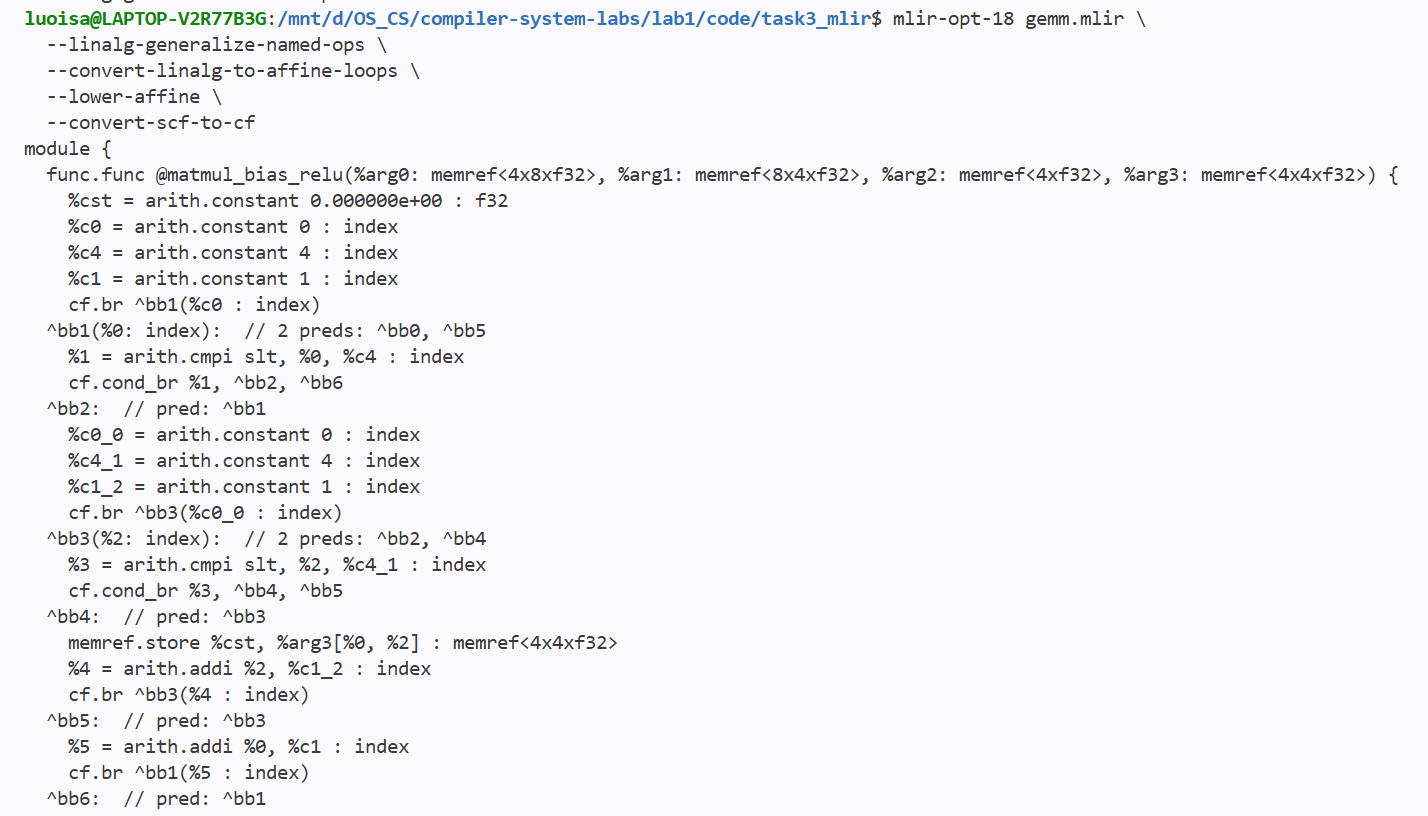
\includegraphics[width=0.92\textwidth]{advanced/05.png}
  \caption{scf.for 被下降为 cf.br/cf.cond\_br 基本块控制流图}
  \label{fig:mlir-04}
\end{figure}

循环变量不再由 scf.for 自动维护，而是\textbf{作为基本块参数}在块之间显式传递（如节选里的 \%0、\%2），并靠 arith.addi 自行累加。对照阶段三可以清楚看到：\textbf{同样的循环语义，在 scf 层是一条指令，在 cf 层则是若干基本块和跳转}。这一层已经非常接近 LLVM IR 的形态。

\hfour{6、阶段五：全部方言下降为 LLVM 方言}

\begin{lstlisting}[language=bash]
mlir-opt-18 gemm.mlir \
  --linalg-generalize-named-ops \
  --convert-linalg-to-affine-loops \
  --lower-affine \
  --convert-scf-to-cf \
  --convert-to-llvm \
  --reconcile-unrealized-casts
\end{lstlisting}

--convert-to-llvm 借助各方言注册的\textbf{转换接口}，把 func、arith、memref、cf、index 等一并换成 llvm 方言；--reconcile-unrealized-casts 则清理转换过程中产生的临时“未实现类型转换”占位操作，输出如图~\ref{fig:mlir-05} 所示。真实输出中，函数签名发生了有趣的变化（节选）：

\begin{lstlisting}[language=MLIR]
  llvm.func @matmul_bias_relu(%arg0: !llvm.ptr, %arg1: !llvm.ptr, %arg2: i64, ..., %arg25: i64) {
    %0 = llvm.mlir.undef : !llvm.struct<(ptr, ptr, i64, array<2 x i64>, array<2 x i64>)>
    %1 = llvm.insertvalue %arg0, %0[0] : !llvm.struct<...>
    ...
\end{lstlisting}

\begin{figure}[H]
  \centering
  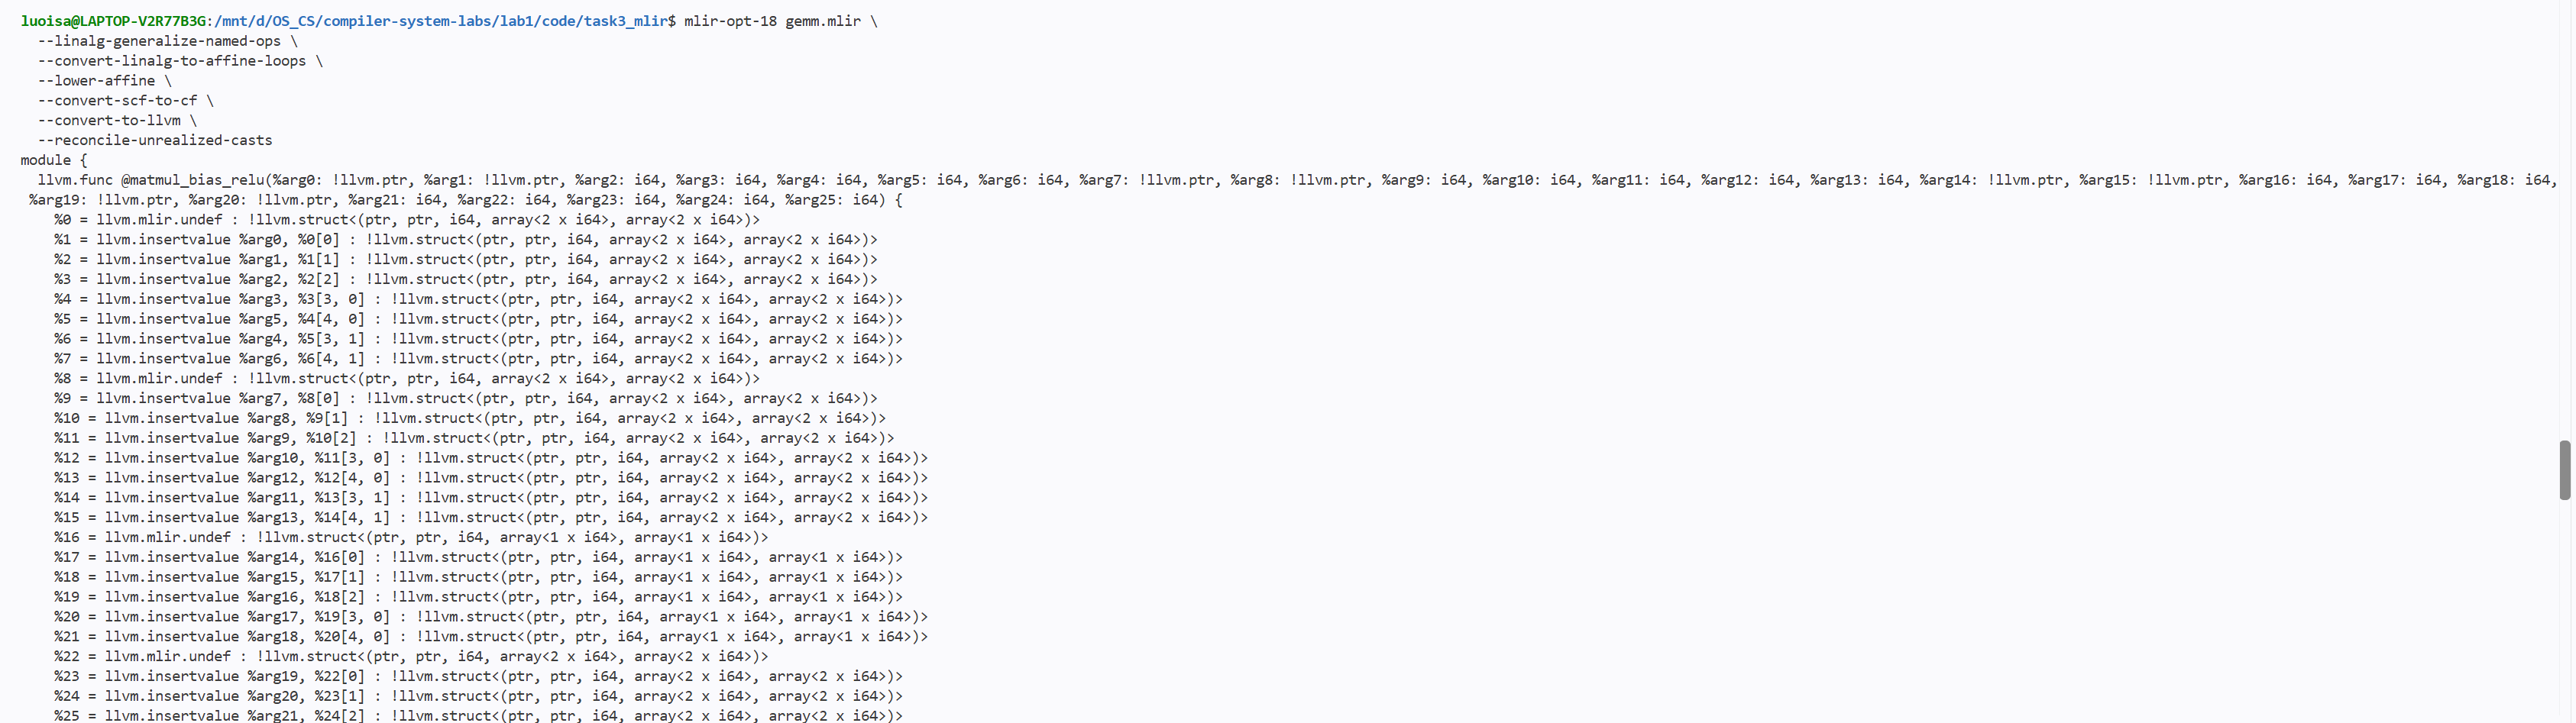
\includegraphics[width=0.92\textwidth]{advanced/06.png}
  \caption{各方言被下降为 llvm 方言，memref 参数展开为描述符字段}
  \label{fig:mlir-05}
\end{figure}

一个 memref<4x8xf32> 参数，落到 LLVM 方言后\textbf{从 1 个参数变成了 6 个}——因为 memref 的底层是“基址指针 + 对齐指针 + 偏移 + 各维大小 + 各维步长”这样的\textbf{描述符（descriptor）结构体}，必须逐字段展开传入。同时，原来的 memref.load/store 变成了 llvm.getelementptr 加 llvm.load/store，循环变量也统一成了 i64：

\begin{lstlisting}[language=MLIR]
    %41 = llvm.mlir.constant(4 : index) : i64
    %42 = llvm.mul %34, %41  : i64
    %43 = llvm.add %42, %39  : i64
    %44 = llvm.getelementptr %arg20[%43] : (!llvm.ptr, i64) -> !llvm.ptr, f32
    llvm.store %30, %44 : f32, !llvm.ptr
\end{lstlisting}

\hfour{7、阶段六：LLVM 方言桥接为真正的 LLVM IR}

\begin{lstlisting}[language=bash]
mlir-translate-18 --mlir-to-llvmir out/05_llvm.mlir > out/06_module.ll
\end{lstlisting}

mlir-translate 负责把 MLIR 的 llvm 方言翻译成标准的 LLVM IR 文本（.ll），至此\textbf{MLIR 的中端旅程结束，交棒给 LLVM 后端}。真实输出的 06\_module.ll 顶部与循环段如下（节选）：

\begin{lstlisting}[language=LLVM]
define void @matmul_bias_relu(ptr %0, ptr %1, i64 %2, ... , i64 %25) {
  %27 = insertvalue { ptr, ptr, i64, [2 x i64], [2 x i64] } undef, ptr %0, 0
  ...
  br label %53

53:                                               ; preds = %65, %26
  %54 = phi i64 [ %66, %65 ], [ 0, %26 ]
  %55 = icmp slt i64 %54, 4
  br i1 %55, label %56, label %67
  ...
\end{lstlisting}

注意两点：\textbf{其一}，llvm.br 在这里变回了 LLVM IR 的 br，并且出现了 phi 节点（\%54 = phi i64 [ \%66, \%65 ], [ 0, \%26 ]）——这正是 SSA 形式对“基本块参数”的等价表达，与任务二“SSA 与 PHI 节点”的原理完全一致；\textbf{其二}，arith.maximumf 最终落成了对 @llvm.maximum.f32 的调用：

\begin{lstlisting}[language=LLVM]
  %118 = call float @llvm.maximum.f32(float %117, float 0.000000e+00)
\end{lstlisting}

这说明 MLIR 里的一个高层算术操作，在下降到 LLVM 时会\textbf{选择最合适的低层内建函数/指令}来实现，跨层语义的映射关系清晰可见。

\hfour{全阶段一次性脚本}

为了方便复现，我把全阶段命令集中写在 run.sh 中。执行 bash run.sh 会一次性生成从 00\_input.mlir 到 09\_ir\_after\_all.log 的全部产物，末行输出 ALL STAGES DONE，如图~\ref{fig:mlir-run} 所示。

\begin{figure}[H]
  \centering
  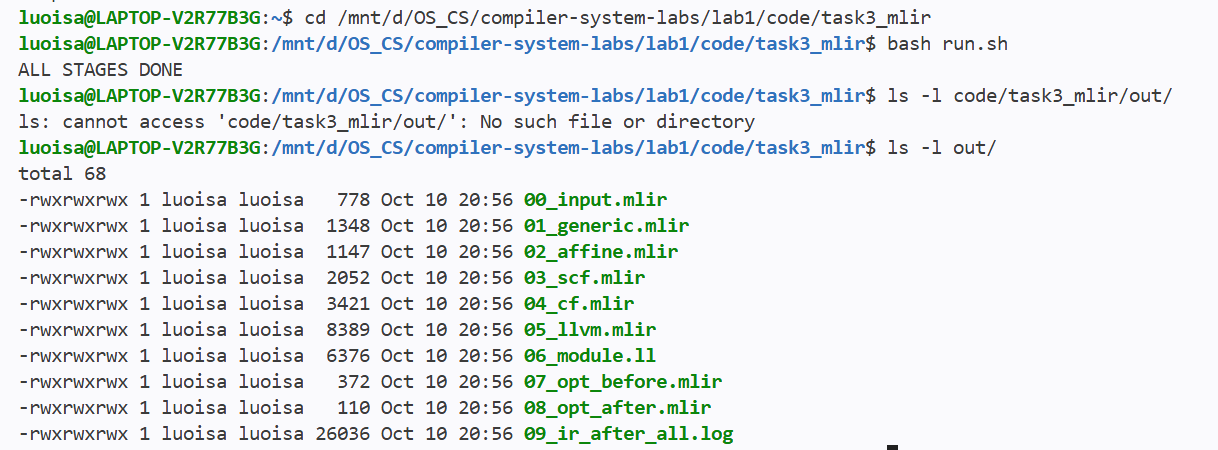
\includegraphics[width=0.92\textwidth]{advanced/3.png}
  \caption{执行 run.sh 一次性生成全部阶段产物，末行提示 ALL STAGES DONE}
  \label{fig:mlir-run}
\end{figure}

\subsubsection{中端优化的观察}

上一小节看到的是“下降”，本小节专门观察“优化”。样例 const\_fold.mlir 故意写了一段包含\textbf{常量运算、公共子表达式与无用计算}的程序：

\begin{lstlisting}[language=MLIR]
func.func @fold() -> i32 {
  %a = arith.constant 3 : i32
  %b = arith.constant 5 : i32
  %c = arith.muli %a, %b : i32          // 3 * 5 = 15
  %d = arith.addi %c, %a : i32          // 15 + 3 = 18
  %e = arith.muli %a, %b : i32          // 与 %c 相同的表达式（可供 CSE 消除）
  %f = arith.addi %d, %e : i32          // 18 + 15 = 33
  %g = arith.muli %f, %a : i32          // 33 * 3 = 99
  %unused = arith.addi %g, %b : i32     // 计算结果无人使用（死代码）
  return %f : i32
}
\end{lstlisting}

优化前后各导出一次：

\begin{lstlisting}[language=bash]
mlir-opt-18 const_fold.mlir > out/07_opt_before.mlir
mlir-opt-18 const_fold.mlir --canonicalize --cse > out/08_opt_after.mlir
\end{lstlisting}

生成的两份文件对比如图~\ref{fig:mlir-opt} 所示。

\begin{figure}[H]
  \centering
  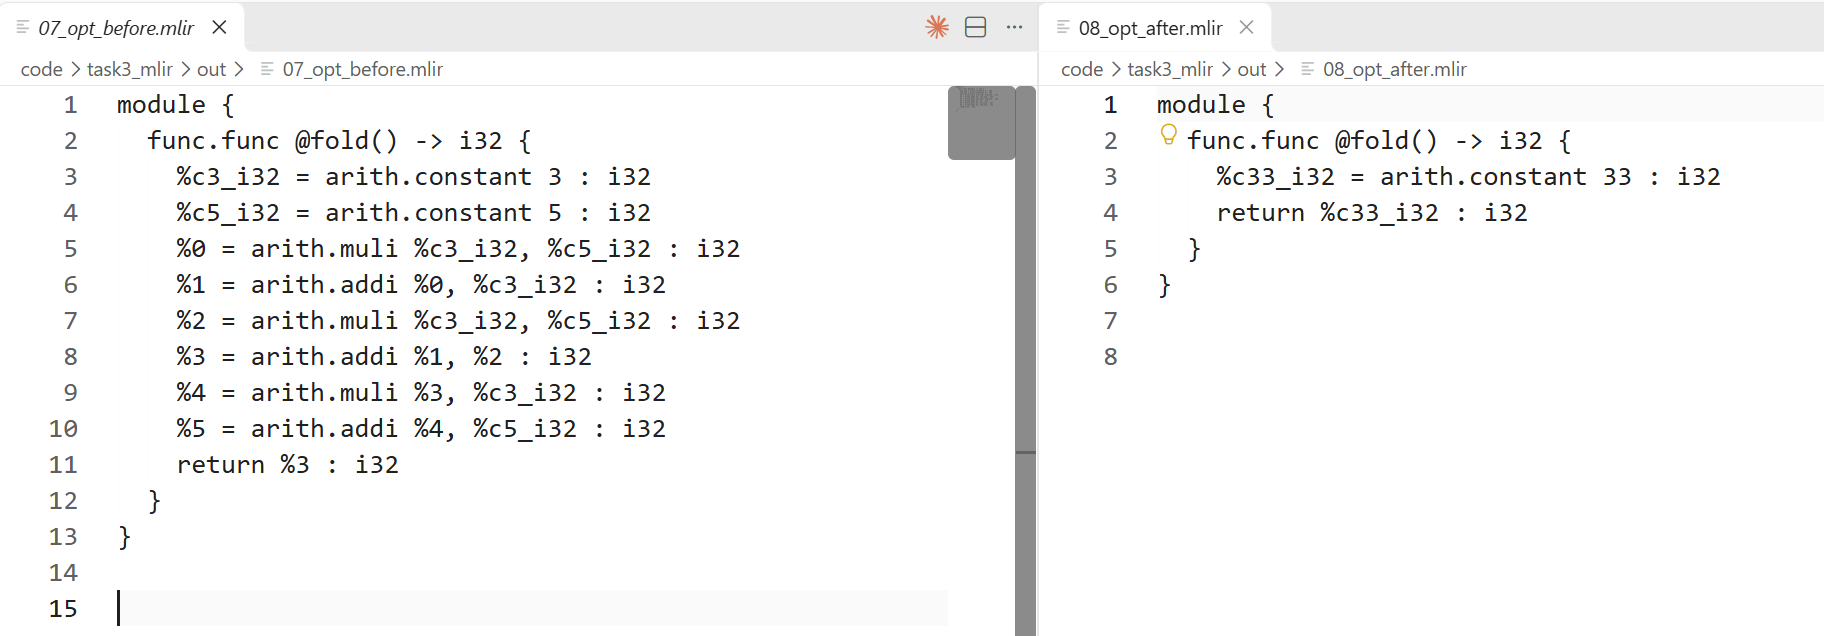
\includegraphics[width=0.92\textwidth]{advanced/07.png}
  \caption{优化前 07\_opt\_before.mlir 与优化后 08\_opt\_after.mlir 的对比}
  \label{fig:mlir-opt}
\end{figure}

\noindent\textbf{优化前}（07\_opt\_before.mlir）——表达式原样保留：

\begin{lstlisting}[language=MLIR]
    %0 = arith.muli %c3_i32, %c5_i32 : i32
    %1 = arith.addi %0, %c3_i32 : i32
    %2 = arith.muli %c3_i32, %c5_i32 : i32
    %3 = arith.addi %1, %2 : i32
    %4 = arith.muli %3, %c3_i32 : i32
    %5 = arith.addi %4, %c5_i32 : i32
    return %3 : i32
\end{lstlisting}

\noindent\textbf{优化后}（08\_opt\_after.mlir）——整段被折叠成一个常量，\%g、\%unused 被作为死代码删除：

\begin{lstlisting}[language=MLIR]
    %c33_i32 = arith.constant 33 : i32
    return %c33_i32 : i32
\end{lstlisting}

这一步里同时发生了三种典型的中端优化，可以逐一对照，如表~\ref{tab:mlirpass} 所示。

\begin{table}[H]
  \centering
  \small
  \setlength{\tabcolsep}{4pt}
  \begin{tabular}{>{\centering\arraybackslash}p{4.0cm}>{\centering\arraybackslash}p{5.3cm}>{\centering\arraybackslash}p{5.3cm}}
    \toprule
\headcol 优化 & \headcol 作用点 & \headcol 效果 \\
    \midrule
常量折叠（constant folding） & arith.muli/arith.addi 的操作数都是常量 & 3*5=15、15+3=18、18+15=33 直接算出 \\
    公共子表达式消除（CSE，--cse） & \%e 与 \%c 是同一表达式 & 合并为一个值 \\
    死代码消除（DCE，--canonicalize 的一部分） & \%g、\%unused 的结果未被使用 & 连同 \%unused 一起删除 \\
    \bottomrule
\end{tabular}
  \caption{一次 --canonicalize --cse 中同时发生的三种优化}
  \label{tab:mlirpass}
\end{table}

\textbf{这正是“中端”的价值所在}：它不改变程序语义，却能让结果从 6 条运算骤减为 0 条运算。在 AI 编译器中，同类的优化（算子融合、常量传播、无用计算删除）规模要大成千上万倍，但道理完全相同。

\subsubsection{用 --mlir-print-ir-after-all 观察 pass 时间线}

前面各阶段是“人为分步导出”的；而在实际工程中，通常一次性把整条流水线交给 mlir-opt，再用打印选项观察每个 pass 之后 IR 的自动变化：

\begin{lstlisting}[language=bash]
mlir-opt-18 gemm.mlir \
  --linalg-generalize-named-ops \
  --convert-linalg-to-affine-loops \
  --lower-affine \
  --convert-scf-to-cf \
  --convert-to-llvm \
  --reconcile-unrealized-casts \
  --mlir-print-ir-after-all > /dev/null 2> out/09_ir_after_all.log
\end{lstlisting}

生成的日志文件如图~\ref{fig:mlir-timeline} 所示。

\begin{figure}[H]
  \centering
  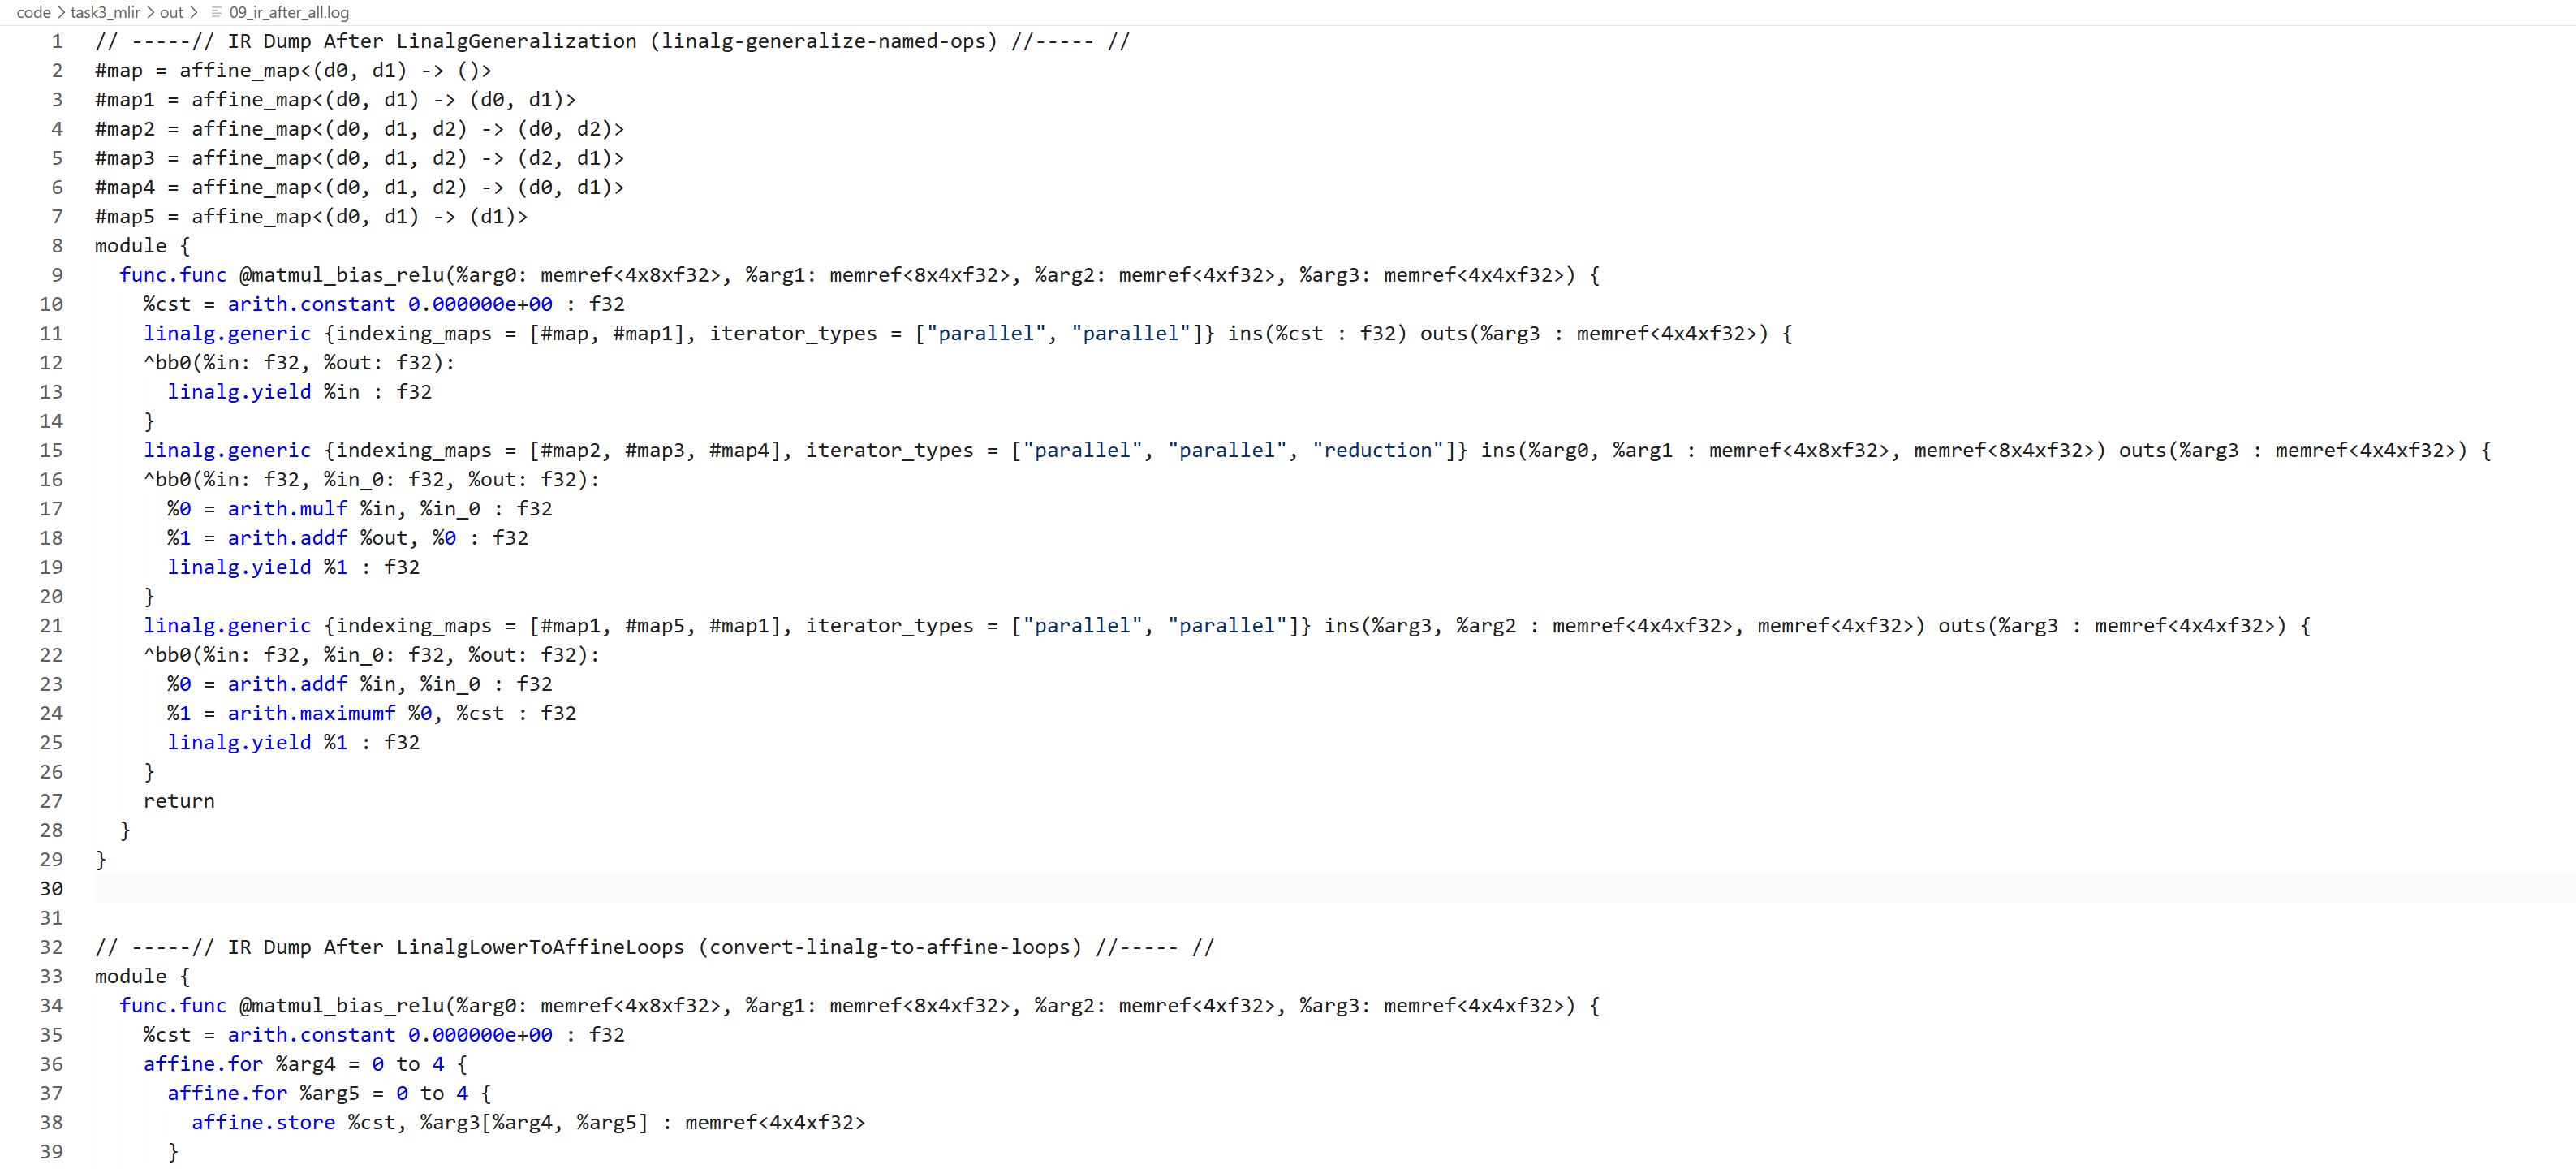
\includegraphics[width=0.92\textwidth]{advanced/08.png}
  \caption{09\_ir\_after\_all.log：每个 pass 之后的 IR 转储与分隔标题}
  \label{fig:mlir-timeline}
\end{figure}

输出文件中，每个 pass 之后都有一段以注释分隔的转储（真实输出的分隔标题）：

\begin{lstlisting}
// -----// IR Dump After LinalgGeneralization (linalg-generalize-named-ops) //----- //
// -----// IR Dump After LinalgLowerToAffineLoops (convert-linalg-to-affine-loops) //----- //
// -----// IR Dump After ConvertAffineToStandard (lower-affine) //----- //
// -----// IR Dump After SCFToControlFlow (convert-scf-to-cf) //----- //
// -----// IR Dump After ConvertToLLVMPass (convert-to-llvm) //----- //
// -----// IR Dump After ReconcileUnrealizedCasts (reconcile-unrealized-casts) //----- //
\end{lstlisting}

这六行标题就是一条\textbf{完整的 pass 时间线}。它把“中端处理”从“一次黑盒运行”变成了“一串可逐步审视的快照”——\textbf{这正是本进阶要求所期望的观察方式}。若在命令行加上 --mlir-print-ir-before-all，则每个 pass 的前后形态可以两两对照；加 --mlir-print-ir-after-change，则只会打印真正产生改动的 pass，便于在长流水线中快速定位“是谁改写了 IR”。

\subsection{实验分析}

\subsubsection{各阶段 IR 的形态与方言对照}

把逐阶段下降的六个阶段汇总，如表~\ref{tab:mlirstages} 所示。

\begin{table}[H]
  \centering
  \small
  \setlength{\tabcolsep}{4pt}
  \begin{tabular}{>{\centering\arraybackslash}p{1.5cm}>{\centering\arraybackslash}p{3.2cm}>{\centering\arraybackslash}p{2.5cm}>{\centering\arraybackslash}p{3.5cm}>{\centering\arraybackslash}p{3.5cm}}
    \toprule
\headcol 阶段 & \headcol 命令 & \headcol 主要方言 & \headcol IR 形态（以矩阵乘为例） & \headcol 关键变化 \\
    \midrule
0 输入 & （无） & func/linalg/memref & linalg.matmul & 高层算子，一句顶三重循环 \\
    1 泛化 & --linalg-generalize-named-ops & linalg & linalg.generic 加循环体 & 并行/归约维被显式标注 \\
    2 降循环 & --convert-linalg-to-affine-loops & affine & 三重 affine.for & 自动生成仿射循环嵌套 \\
    3 去仿射 & --lower-affine & scf/memref & 三重 scf.for & 仿射下标退化为普通下标访问 \\
    4 降 CFG & --convert-scf-to-cf & cf & 基本块加 cf.cond\_br & 结构化循环被摊平为控制流图 \\
    5 降 LLVM & --convert-to-llvm & llvm & llvm.getelementptr/load/store & 描述符展开、类型统一为 i64 \\
    6 转 IR & mlir-translate & LLVM IR & br/phi/getelementptr & 接入 LLVM 后端，出现 PHI 节点 \\
    \bottomrule
\end{tabular}
  \caption{渐进式下降各阶段的 IR 形态与关键变化}
  \label{tab:mlirstages}
\end{table}

可以看出一个非常干净的规律：\textbf{每经过一个 pass，IR 就“更低一层”，可用的高层信息就更少，与机器码的距离就更近。}而每一层都保留了完整的程序语义，可以在任意一层插入针对该层的优化。

\subsubsection{方言分层带来的“一处编写、多级复用”}

MLIR 的设计精髓在于：\textbf{每一层只关心自己那一层的抽象，并只把必要的结构信息向下传递。}例如 linalg 层用 indexing\_maps 与 iterator\_types 描述了算子的并行/归约结构，正是这份“高层结构”让 --convert-linalg-to-affine-loops 得以\textbf{自动}生成循环——编写者不必手写循环，只要把算子的语义描述清楚。

这带来两个直接收益：

\begin{itemize}
  \item \textbf{其一，可组合。} 同一份 linalg 算子，可以配不同的下降路线（降到 affine 做多面体优化，或降到 gpu 方言做 GPU 并行化），不必重写。
  \item \textbf{其二，可复用。} 通用的 pass（如 --canonicalize、--cse）可以作用在任意方言上，只要方言实现了相应接口；新硬件只需提供自己的方言与下降路线，无须改动前端。
\end{itemize}

这与任务二“前端只管产出 LLVM IR、后端只管消费 LLVM IR”的两段式思想一脉相承，只是 MLIR 把中间的“一段”进一步细分成“多级”，以适应 AI 编译器更复杂的优化需求。

\subsubsection{MLIR 中端与经典编译流程的位置关系}

把本次进阶实验与任务一、任务二放在一张图上，如代码~\ref{code:position} 所示。

\begin{lstlisting}[label=code:position]
       任务二（手写 IR）                本实验（AI 编译器中端）              任务一（GCC 四阶段）
   SysY/C --clang--> LLVM IR       模型 --前端--> linalg --[多级下降]--> LLVM IR --llc--> .s --as--> .o --ld--> 可执行
                          ^                        ^                         ^
                          +---------- 二者在 LLVM IR 处汇合 ----------------+
\end{lstlisting}

也就是说，\textbf{MLIR 的中端处理，本质上是在“前端”与“LLVM 后端”之间插入的一段可编程、可分层的优化流水线}：它接手的是 AI 框架导出的高层算子图，交付的是标准 LLVM IR。任务二让我们看到了“LLVM IR 长什么样”，本进阶实验则让我们看到了“LLVM IR 之前还发生了什么”——两者在 06\_module.ll 这一步严丝合缝地接上了。

\subsection{小结}

通过本进阶实验，完成了从"写中间代码"到"观察中间代码被如何变换"的视角转换，主要收获如下：

\begin{enumerate}[1.]
  \item \textbf{理解了 MLIR 的核心主张。} 用"方言"把 IR 分层，用"渐进式下降"把高层算子逐级变为机器码；Operation、Dialect、Pass 三个概念构成整套体系的地基。

  \item \textbf{完整走通了一条下降路线。} linalg 依次经 affine、scf、cf、llvm 各层到达 LLVM IR，每一级的 IR 形态都取到了真实证据；下降终点恰好接上任务二的 LLVM IR，可由 llc 继续生成机器码。

  \item \textbf{掌握了观察中端与复现优化的方法。} 通过 --mlir-print-ir-after-all 等选项配合 mlir-translate，无需插桩即可逐步打开"中端"；在 --canonicalize --cse 下复现了常量折叠、公共子表达式消除与死代码消除，6 条运算被折叠为 0 条。
\end{enumerate}

\section{总结}

通过本次实验，我们对自己的编译器、LLVM IR 编程以及 RISC-V 汇编编程有了更加深刻的理解。

从任务一中，我们首先了解了完整的编译过程，然后分步骤对其进行探究，其中包括预处理阶段的功能、编译器中的六大步骤——词法分析、语法分析、语义分析、中间代码生成、代码优化、目标代码生成，以及汇编器、链接器和程序的执行流程。在预处理器阶段，我们验证了头文件展开、宏定义替换与注释去除等功能；在编译阶段，通过词法分析了解到记号序列的生成，通过语法分析了解到抽象语法树的构造与语法检查功能，通过语义分析了解到类型检查与符号表的构建，通过中间代码生成了解到控制流图的表示，通过代码优化观察到 -O0 与 -O2 之间的巨大差异，通过目标代码生成了解到 LLVM、x86 等形式的目标代码；在汇编阶段，我们分析了节区组织、符号表与重定位表；在链接阶段，我们分析了符号解析、重定位填补以及 PLT/GOT 动态链接机制，最后通过执行程序完成了整个流程。

从任务二中，我们编写了 LLVM IR 程序并进行了优化和探索。首先根据斐波那契数列程序学习了 LLVM IR 语言的基本写法，在此基础上对程序做了数组与算术运算的扩展，并使用 alloca 内存模型、getelementptr 地址计算、SSA 与 PHI 节点等特性完成了完整的手写 IR，最后通过与 C 版本逐字节比对验证了语义等价性。同时将手写 IR 与 Clang 自动生成的 -O0/-O2 版本对照，分析了常量折叠、循环求值等优化技术。

从任务三中，我们编写了两个 RISC-V 汇编程序。首先是斐波那契数列程序，通过 SysY 源程序明确了汇编编写思路，包括程序的输出、栈帧分配以及寄存器分工，然后逐行编写并分析了汇编程序，使用交叉编译器编译并在 QEMU 上运行验证，输出正确。第二个程序是参数超过 8 个的函数程序，专门考察了栈上传参的调用约定，通过推导与运行结果交叉验证了正确性。

从进阶要求中，我们观察了 AI 编译器 MLIR 的中端处理过程，让一个矩阵乘加 ReLU 的 MLIR 样例依次流经从 linalg 方言到 LLVM 方言的完整下降流水线，逐阶段转储并分析了中间表示的变化，复现了常量折叠、公共子表达式消除与死代码消除等中端优化。

四个任务在 LLVM IR 这一层汇合：任务一让我们看到编译器如何生成 LLVM IR，任务二让我们亲手编写 LLVM IR，任务三让我们看到 LLVM IR 如何进一步降到汇编，进阶实验则让我们看到 LLVM IR 之前还发生了什么。本次实验让我们认识到编译器是一系列职责清晰、接口明确的小程序的有序组合，而这套"分层 + 约定 + 验证"的思维方式，也正是我们后续学习编译系统设计的起点。

\newpage

\newpage
\section{参考文献}



[1] Aho A V, Lam M S, Sethi R, Ullman J D. Compilers: Principles, Techniques, and Tools[M]. 2nd ed. Boston: Addison-Wesley, 2006. ISBN 978-0-321-48681-3.

[2] 全国大学生计算机系统能力大赛组织委员会. 2021 年全国大学生计算机系统能力大赛编译系统设计赛技术方案（含 SysY2021 语言定义）[S/OL]. 2021. \url{https://course.educg.net/userfiles/markdown/CONTEST/file/2021_3/1ll1616058425.pdf.}


[3] Free Software Foundation. GNU Compiler Collection (GCC) Internals[EB/OL]. \url{https://gcc.gnu.org/onlinedocs/gccint/.}

[4] Free Software Foundation. Developer Options（\texttt{-fdump-tree-*} 等）[EB/OL]. \url{https://gcc.gnu.org/onlinedocs/gcc/Developer-Options.html.}

[5] LLVM Project. LLVM Language Reference Manual[EB/OL]. \url{https://llvm.org/docs/LangRef.html.}


[6] Free Software Foundation. The GNU Linker (GNU Binutils)[EB/OL]. \url{https://sourceware.org/binutils/docs/ld/.}

[7] Tool Interface Standard (TIS) Committee. Executable and Linkable Format (ELF) Specification, Version 1.2[S]. 1995. \url{https://refspecs.linuxfoundation.org/elf/.}

[8] x86 psABIs. System V Application Binary Interface: AMD64 Architecture Processor Supplement (With LP64 and ILP32 Programming Models)[S/OL]. \url{https://gitlab.com/x86-psABIs/x86-64-ABI.}

[9] RISC-V International. The RISC-V Instruction Set Manual, Volume I: Unprivileged Architecture[S/OL]. \url{https://docs.riscv.org/reference/isa/unpriv/unpriv-index.html.}

[10] RISC-V Non-ISA Specifications. RISC-V ELF psABI Specification[S/OL]. \url{https://github.com/riscv-non-isa/riscv-elf-psabi-doc.}


[11] Lattner C, Amini M, Bondhugula U, et al. MLIR: Scaling Compiler Infrastructure for Domain Specific Computation[C]//2021 IEEE/ACM International Symposium on Code Generation and Optimization (CGO). IEEE, 2021: 2-14. DOI: 10.1109/CGO51591.2021.9370308.

[12] LLVM Project. MLIR Documentation[EB/OL]. \url{https://mlir.llvm.org/docs/.}

\newpage
\section{附录}
\subsection{附录 A　实验环境与工具版本一览}


\begin{table}[H]
  \centering
  \small
  \setlength{\tabcolsep}{4pt}
  \begin{tabular}{>{\centering\arraybackslash}p{2.5cm}>{\centering\arraybackslash}p{3.2cm}>{\centering\arraybackslash}p{3.2cm}>{\centering\arraybackslash}p{3.2cm}>{\centering\arraybackslash}p{3.2cm}}
    \toprule
    \headcol 项目 & \headcol 任务一（四阶段） & \headcol 任务二（LLVM IR） & \headcol 任务三（RISC-V 汇编） & \headcol 进阶（MLIR 中端） \\
    \midrule
    操作系统 & Windows + WSL2，Ubuntu，内核 6.6.114.1 & Windows + WSL2，Ubuntu & WSL2 Ubuntu，Linux 6.6 & Windows + WSL2，Ubuntu 24.04.4 LTS \\
    C 编译器（前端） & GCC 15.2.0 / Clang 21.1.8 & Clang 18.1.3 & \texttt{riscv64-linux-gnu-gcc}（GCC 15.2.0） & Clang 18.1.3 \\
    中间代码工具 & LLVM 21.1.8（\texttt{llvm-as}、\texttt{opt}、\texttt{llc}） & LLVM 18.1.3（\texttt{llvm-as}、\texttt{llvm-dis}、\texttt{opt}、\texttt{llc}） & — & \textbf{MLIR 18.1.3}（\texttt{mlir-opt-18}、\texttt{mlir-translate-18}） \\
    汇编器 / 链接器 & GNU \texttt{as}、\texttt{ld}（随 GCC 15.2.0） & — & \texttt{riscv64-linux-gnu-as}、\texttt{riscv64-linux-gnu-ld} & — \\
    目标架构 & x86-64（System V ABI） & x86-64 & RV64GC（\texttt{rv64i}+\texttt{m}+\texttt{a}+\texttt{f}+\texttt{d}+\texttt{c}），\texttt{lp64d} & x86-64 \\
    模拟器 & — & — & \texttt{qemu-riscv64} 10.2.1 & — \\
    可视化 & Graphviz 14.1.2（\texttt{dot}） & — & — & — \\
    编辑 / 终端 & VSCode + WSL 集成终端 & 同上 & 同上 & 同上 \\
    \bottomrule
  \end{tabular}
\end{table}


\begin{quote}
说明：任务一由 GCC 与 Clang 两套工具链分别取证，故版本号并列；任务二任务三所依据的 SysY 示例程序在校验前已由两名组员共同冻结。
\end{quote}



\subsection{附录 B　复现命令清单}


以下命令均在 WSL 中执行；\texttt{\$} 为提示符，复制时请省略。

\subsubsection{B.1　任务一：GCC / Clang 四阶段观测}


\begin{lstlisting}[language=bash]
cd code/task1_compiler

# 预处理：C 源程序 -> 预处理文件
gcc src/main.c -E -o outputs/main.i

# 词法分析：打印记号流
clang -E -Xclang -dump-tokens src/main.c

# 语法分析：打印抽象语法树
clang -E -Xclang -ast-dump src/main.c

# 编译到 LLVM 中间代码（-O0），再到优化版本与目标汇编
clang -S -emit-llvm src/main.c -o outputs/main.ll
llvm-as outputs/main.ll -o outputs/main.bc
opt -S -O1 outputs/main.bc -o outputs/main-O1.ll
opt -S -O2 outputs/main.bc -o outputs/main-O2.ll
opt -S -O3 outputs/main.bc -o outputs/main-O3.ll
clang -O2 -S -emit-llvm src/main.c -o outputs/main-clangO2.ll
llc outputs/main.ll -o outputs/main-llvm.S

# GCC 内部 GIMPLE / 优化后 SSA
gcc -fdump-tree-gimple src/main.c
gcc -fdump-tree-optimized -O2 src/main.c

# 编译到汇编
gcc src/main.c -S -o outputs/main.s

# 汇编：汇编文本 -> 可重定位目标文件
as outputs/main.s -o outputs/main.o

# 观察目标文件：ELF 头、节表、符号表、重定位表、反汇编
readelf -h outputs/main.o
readelf -S outputs/main.o
readelf -s outputs/main.o
readelf -r outputs/main.o
objdump -d outputs/main.o

# 链接：目标文件 -> 可执行文件
gcc outputs/main.o -o outputs/main
ld outputs/main.o -o /tmp/t          # 故意触发 undefined reference

# 观察可执行文件
file outputs/main
readelf -h outputs/main
readelf -l outputs/main
readelf -d outputs/main
readelf -r outputs/main
readelf -s outputs/main
objdump -d outputs/main

# 静态链接对照
gcc -static outputs/main.o -o outputs/main_static\end{lstlisting}


\subsubsection{B.2　任务二：LLVM IR 与 SysY}


\begin{lstlisting}[language=bash]
cd code/task2_llvm

# 语法与类型检查（能通过即 IR 合法）
llvm-as demo.ll -o /dev/null && echo "llvm-as: OK"

# 手写 IR 与运行库一起编译、运行
clang demo.ll sylib.c -o demo_ir
./demo_ir

# 与期望输出逐字节比对
./demo_ir > actual.txt
diff expected.txt actual.txt && echo "MATCH"

# 生成 Clang 自动 IR 用于对照（-O0 / -O2）
clang -O0 -emit-llvm -S -include syhdr.h demo.c -o auto_O0.ll
clang -O2 -emit-llvm -S -include syhdr.h demo.c -o auto_O2.ll

# 或使用 Makefile 一键复现：make / make check / make auto\end{lstlisting}


\subsubsection{B.3　任务三：RISC-V 汇编}


\begin{lstlisting}[language=bash]
cd code/task3_asm/program1_demo

# 交叉汇编 + 静态链接 + QEMU 运行（务必使用 /usr/bin/qemu-riscv64，见下）
riscv64-linux-gnu-gcc -march=rv64gc -mabi=lp64d -static \
    demo.s sysy_runtime.c -o demo_riscv
/usr/bin/qemu-riscv64 ./demo_riscv

# 交叉编译同一份 demo.c，生成对照汇编并运行
riscv64-linux-gnu-gcc -S -march=rv64gc -mabi=lp64d -fno-stack-protector demo.c -o demo_gcc.s
riscv64-linux-gnu-gcc -march=rv64gc -mabi=lp64d -static demo_gcc.s sysy_runtime.c -o demo_gcc
/usr/bin/qemu-riscv64 ./demo_gcc

# 程序二：超过 8 个参数的函数
cd ../program2_multiarg
riscv64-linux-gnu-gcc -march=rv64gc -mabi=lp64d -static manyargs.s sysy_runtime.c -o manyargs
/usr/bin/qemu-riscv64 ./manyargs\end{lstlisting}


\subsubsection{B.4　进阶要求：MLIR 中端处理}


\begin{lstlisting}[language=bash]
cd code/task3_mlir
bash run.sh          # 一条命令复现报告中的全部 MLIR 中端处理结果，输出写入 out/\end{lstlisting}


\texttt{run.sh} 依次执行：解析输入（\texttt{00\_input}）、具名算子展开（\texttt{01\_generic}）、linalg → affine（\texttt{02\_affine}）、affine → scf（\texttt{03\_scf}）、scf → cf（\texttt{04\_cf}）、全方言 → LLVM（\texttt{05\_llvm}）、LLVM 方言 → LLVM IR（\texttt{06\_module.ll}）、中端优化前后对照（\texttt{07/08}），并用 \texttt{--mlir-print-ir-after-all} 输出逐 pass 时间线（\texttt{09\_ir\_after\_all.log}）。





\subsection{附录 C　源程序与关键产物清单}


\subsubsection{C.1　\texttt{code/task1\_compiler/src/main.c}（任务一分析对象）}


\begin{lstlisting}[language=C]
#include <stdio.h>
#define MAX 100

int main() {
    int i, n, f;
    scanf("%d", &n);
    i = 2;
    f = 1;
    while (i <= n) {
        f = f * i;
        i = i + 1;
    }
    printf("%d\n", f);
    return 0;
}\end{lstlisting}


\subsubsection{C.2　\texttt{code/task2\_llvm/demo.c}（任务二/三共用的 SysY 示例程序）}


\begin{lstlisting}[language=C]
const int N = 8;
int calls = 0;

int fib(int n)
{
    if (n <= 1)
        return n;
    calls = calls + 1;
    return fib(n - 1) + fib(n - 2);
}

int calc(int a, int b)
{
    return (a + b) * (a - b) / b + a % b;
}

int main()
{
    int a[5] = {1, 2, 3, 4, 5};
    int i = 0, x = 0, y = 1, t, sum = 0;

    while (i < N)
    {
        if (i < 5)
            a[i] = x;
        t = x + y;
        x = y;
        y = t;
        i = i + 1;
    }

    putint(fib(5));
    putch(10);

    i = 0;
    while (i < 5)
    {
        if (a[i] % 2 == 0)
            sum = sum + a[i];
        else
            sum = sum + 1;
        i = i + 1;
    }

    putarray(5, a);
    putint(sum);
    putch(10);
    putint(calc(7, 3));
    putch(10);
    putint(calls);
    putch(10);

    return 0;
}\end{lstlisting}


\textbf{期望输出（\texttt{expected.txt}）：}

\begin{lstlisting}
5
5: 0 1 1 2 3
5
14
7\end{lstlisting}


\subsubsection{C.3　\texttt{code/task2\_llvm/sylib.c} 与 \texttt{syhdr.h}（任务二运行库）}


\begin{lstlisting}[language=C]
/* sylib.c */
#include <stdio.h>

void putint(int a)
{
    printf("%d", a);
}

void putch(int a)
{
    putchar(a);
}

void putarray(int n, int a[])
{
    printf("%d:", n);
    for (int i = 0; i < n; i++)
        printf(" %d", a[i]);
    printf("\n");
}

int getint()
{
    int a;
    scanf("%d", &a);
    return a;
}

int getch()
{
    int a;
    scanf("%d", &a);
    return a;
}

int getarray(int a[])
{
    int n;
    scanf("%d", &n);
    for (int i = 0; i < n; i++)
        scanf("%d", &a[i]);
    return n;
}\end{lstlisting}


\begin{lstlisting}[language=C]
/* syhdr.h */
void putint(int);
void putch(int);
void putarray(int, int[]);
int getint(void);
int getch(void);
int getarray(int[]);\end{lstlisting}


\subsubsection{C.4　\texttt{code/task2\_llvm/demo.ll}（手写 LLVM IR 全文）}


\begin{lstlisting}[language=LLVM]
; Hand-written LLVM IR equivalent to demo.c

target triple = "x86_64-pc-linux-gnu"

; --- 全局变量 ---
@N = constant i32 8                              ; const int N = 8
@calls = global i32 0                            ; int calls = 0

; --- 运行库函数声明 ---
declare void @putint(i32)
declare void @putch(i32)
declare void @putarray(i32, ptr)

; ============================================================
; int fib(int n)
; ============================================================
define i32 @fib(i32 %n) {
entry:
  %n.addr = alloca i32, align 4
  store i32 %n, ptr %n.addr, align 4
  %0 = load i32, ptr %n.addr, align 4
  %cmp = icmp sle i32 %0, 1
  br i1 %cmp, label %if.then, label %if.end

if.then:                                          ; n <= 1
  %1 = load i32, ptr %n.addr, align 4
  ret i32 %1

if.end:                                           ; n > 1
  %2 = load i32, ptr @calls, align 4
  %inc = add nsw i32 %2, 1
  store i32 %inc, ptr @calls, align 4
  %3 = load i32, ptr %n.addr, align 4
  %sub1 = sub nsw i32 %3, 1
  %call1 = call i32 @fib(i32 %sub1)
  %4 = load i32, ptr %n.addr, align 4
  %sub2 = sub nsw i32 %4, 2
  %call2 = call i32 @fib(i32 %sub2)
  %add = add nsw i32 %call1, %call2
  ret i32 %add
}

; ============================================================
; int calc(int a, int b)
; ============================================================
define i32 @calc(i32 %a, i32 %b) {
entry:
  %a.addr = alloca i32, align 4
  %b.addr = alloca i32, align 4
  store i32 %a, ptr %a.addr, align 4
  store i32 %b, ptr %b.addr, align 4
  %0 = load i32, ptr %a.addr, align 4
  %1 = load i32, ptr %b.addr, align 4
  %add = add nsw i32 %0, %1
  %2 = load i32, ptr %a.addr, align 4
  %3 = load i32, ptr %b.addr, align 4
  %sub = sub nsw i32 %2, %3
  %mul = mul nsw i32 %add, %sub
  %4 = load i32, ptr %b.addr, align 4
  %div = sdiv i32 %mul, %4
  %5 = load i32, ptr %a.addr, align 4
  %6 = load i32, ptr %b.addr, align 4
  %rem = srem i32 %5, %6
  %add1 = add nsw i32 %div, %rem
  ret i32 %add1
}

; ============================================================
; int main()
; ============================================================
define i32 @main() {
entry:
  %retval = alloca i32, align 4
  %a = alloca [5 x i32], align 4
  %i = alloca i32, align 4
  %x = alloca i32, align 4
  %y = alloca i32, align 4
  %t = alloca i32, align 4
  %sum = alloca i32, align 4
  store i32 0, ptr %retval, align 4

  ; int a[5] = {1, 2, 3, 4, 5};
  %a.0 = getelementptr inbounds [5 x i32], ptr %a, i64 0, i64 0
  store i32 1, ptr %a.0, align 4
  %a.1 = getelementptr inbounds [5 x i32], ptr %a, i64 0, i64 1
  store i32 2, ptr %a.1, align 4
  %a.2 = getelementptr inbounds [5 x i32], ptr %a, i64 0, i64 2
  store i32 3, ptr %a.2, align 4
  %a.3 = getelementptr inbounds [5 x i32], ptr %a, i64 0, i64 3
  store i32 4, ptr %a.3, align 4
  %a.4 = getelementptr inbounds [5 x i32], ptr %a, i64 0, i64 4
  store i32 5, ptr %a.4, align 4

  ; int i = 0, x = 0, y = 1, t, sum = 0;
  store i32 0, ptr %i, align 4
  store i32 0, ptr %x, align 4
  store i32 1, ptr %y, align 4
  store i32 0, ptr %sum, align 4
  br label %while.cond

; ---- while (i < N) ----
while.cond:
  %0 = load i32, ptr %i, align 4
  %1 = load i32, ptr @N, align 4
  %cmp = icmp slt i32 %0, %1
  br i1 %cmp, label %while.body, label %while.end

while.body:
  ; if (i < 5) a[i] = x;
  %2 = load i32, ptr %i, align 4
  %cmp2 = icmp slt i32 %2, 5
  br i1 %cmp2, label %if.then, label %if.end

if.then:
  %3 = load i32, ptr %i, align 4
  %4 = load i32, ptr %x, align 4
  %idx.ext = sext i32 %3 to i64
  %arrayidx = getelementptr inbounds [5 x i32], ptr %a, i64 0, i64 %idx.ext
  store i32 %4, ptr %arrayidx, align 4
  br label %if.end

if.end:
  ; t = x + y;
  %5 = load i32, ptr %x, align 4
  %6 = load i32, ptr %y, align 4
  %add = add nsw i32 %5, %6
  store i32 %add, ptr %t, align 4
  ; x = y;
  %7 = load i32, ptr %y, align 4
  store i32 %7, ptr %x, align 4
  ; y = t;
  %8 = load i32, ptr %t, align 4
  store i32 %8, ptr %y, align 4
  ; i = i + 1;
  %9 = load i32, ptr %i, align 4
  %inc = add nsw i32 %9, 1
  store i32 %inc, ptr %i, align 4
  br label %while.cond

while.end:
  ; putint(fib(5)); putch(10);
  %call = call i32 @fib(i32 5)
  call void @putint(i32 %call)
  call void @putch(i32 10)

  ; i = 0;
  store i32 0, ptr %i, align 4
  br label %while.cond3

; ---- while (i < 5) ----
while.cond3:
  %10 = load i32, ptr %i, align 4
  %cmp3 = icmp slt i32 %10, 5
  br i1 %cmp3, label %while.body3, label %while.end3

while.body3:
  ; if (a[i] % 2 == 0) sum = sum + a[i]; else sum = sum + 1;
  %11 = load i32, ptr %i, align 4
  %idx.ext4 = sext i32 %11 to i64
  %arrayidx4 = getelementptr inbounds [5 x i32], ptr %a, i64 0, i64 %idx.ext4
  %12 = load i32, ptr %arrayidx4, align 4
  %rem5 = srem i32 %12, 2
  %cmp6 = icmp eq i32 %rem5, 0
  br i1 %cmp6, label %if.then7, label %if.else

if.then7:
  %13 = load i32, ptr %sum, align 4
  %14 = load i32, ptr %arrayidx4, align 4
  %add8 = add nsw i32 %13, %14
  store i32 %add8, ptr %sum, align 4
  br label %if.end9

if.else:
  %15 = load i32, ptr %sum, align 4
  %add10 = add nsw i32 %15, 1
  store i32 %add10, ptr %sum, align 4
  br label %if.end9

if.end9:
  ; i = i + 1;
  %16 = load i32, ptr %i, align 4
  %inc11 = add nsw i32 %16, 1
  store i32 %inc11, ptr %i, align 4
  br label %while.cond3

while.end3:
  ; putarray(5, a);
  %arraydecay = getelementptr inbounds [5 x i32], ptr %a, i64 0, i64 0
  call void @putarray(i32 5, ptr %arraydecay)
  ; putint(sum); putch(10);
  %17 = load i32, ptr %sum, align 4
  call void @putint(i32 %17)
  call void @putch(i32 10)
  ; putint(calc(7, 3)); putch(10);
  %call12 = call i32 @calc(i32 7, i32 3)
  call void @putint(i32 %call12)
  call void @putch(i32 10)
  ; putint(calls); putch(10);
  %18 = load i32, ptr @calls, align 4
  call void @putint(i32 %18)
  call void @putch(i32 10)

  ret i32 0
}\end{lstlisting}


\subsubsection{C.5　\texttt{code/task2\_llvm/Makefile}（任务二一键复现）}


\begin{lstlisting}[language=bash]
CC = clang
CFLAGS = -Wall

.PHONY: all check auto clean

all: demo_ir
	./demo_ir

demo_ir: demo.ll sylib.c
	$(CC) demo.ll sylib.c -o demo_ir

check: demo_ir
	./demo_ir > actual.txt
	diff expected.txt actual.txt && echo "PASS: output matches expected.txt"

auto:
	clang -O0 -emit-llvm -S -include syhdr.h demo.c -o auto_O0.ll
	clang -O2 -emit-llvm -S -include syhdr.h demo.c -o auto_O2.ll

clean:
	rm -f demo_ir demo_o2 actual.txt o2_out.txt auto_O0.ll auto_O2.ll *.o\end{lstlisting}


\subsubsection{C.6　\texttt{code/task3\_asm/program1\_demo/sysy.h} 与 \texttt{sysy\_runtime.c}（任务三运行库）}


\begin{lstlisting}[language=C]
/* sysy.h */
#ifndef SYSY_H
#define SYSY_H

/* 输入 */
int getint();
int getch();
int getarray(int a[]);
float getfloat();
int getfarray(float a[]);

/* 输出 */
void putint(int a);
void putch(int a);
void putarray(int n, int a[]);
void putfloat(float a);
void putfarray(int n, float a[]);

/* 计时 */
void starttime();
void stoptime();

#endif\end{lstlisting}


\begin{lstlisting}[language=C]
/* sysy_runtime.c —— SysY 运行时库的简易实现，仅用于本地验证汇编程序 */
#include <stdio.h>

int getint() { int x; scanf("%d", &x); return x; }
int getch() { return getchar(); }
int getarray(int a[]) {
    int n;
    scanf("%d", &n);
    for (int i = 0; i < n; i++) scanf("%d", &a[i]);
    return n;
}

void putint(int a) { printf("%d", a); }
void putch(int a) { putchar(a); }
void putarray(int n, int a[]) {
    printf("%d:", n);
    for (int i = 0; i < n; i++) printf(" %d", a[i]);
    printf("\n");
}\end{lstlisting}


\subsubsection{C.7　手写任务三程序一 RISC-V 全文（\texttt{code/task3\_asm/program1\_demo/demo.s}）}


\begin{lstlisting}[language=riscv]
#==============================================================================
# demo.s —— 与 demo.c 等价的 RISC-V (RV64GC) 汇编程序
#
# 源程序：
#   const int N = 8;
#   int calls = 0;
#   int fib(int n)               —— 递归求斐波那契
#   int calc(int a, int b)       —— 整数四则与取余
#   int main()                   —— 数组、双循环、函数调用与输出
#
# 汇编/链接/运行：
#   riscv64-linux-gnu-gcc -march=rv64gc -mabi=lp64d -static demo.s sysy_runtime.c -o demo_riscv
#   /usr/bin/qemu-riscv64 ./demo_riscv
#
#==============================================================================

    .file   "demo.s"
    .option nopic
    .attribute arch, "rv64i2p1_m2p0_a2p1_f2p2_d2p2_c2p0"
    .attribute unaligned_access, 0
    .attribute stack_align, 16


#------------------------------------------------------------------------------
# 全局数据段
#   N      —— const int，内容不可变，放入只读数据段 .rodata
#   calls  —— int，初值为 0，放入 .bss
#------------------------------------------------------------------------------
    .section .rodata
    .align  2                       # 4 字节对齐，与 int 的自然对齐一致
    .globl  N
    .type   N, @object
    .size   N, 4
N:
    .word   8

    .section .bss
    .align  2
    .globl  calls
    .type   calls, @object
    .size   calls, 4
calls:
    .zero   4


#------------------------------------------------------------------------------
# int fib(int n)
#
# 栈帧布局（sp 为基准，共 32 字节）：
#       24(sp)  ra
#       16(sp)  s1      —— 保存 fib(n-1) 的结果，跨越第二次递归调用
#        8(sp)  n       —— 形参备份
#
# 传参/返回：n 由 a0 传入，返回值由 a0 传出
#------------------------------------------------------------------------------
    .text
    .align  2
    .globl  fib
    .type   fib, @function
fib:
    addi    sp, sp, -32             # 开辟栈帧
    sd      ra, 24(sp)              # 保护返回地址
    sd      s1, 16(sp)              # 保护被调用者保存寄存器 s1
    sw      a0, 8(sp)               # 形参 n 落栈

    # ---- if (n <= 1) return n; ----
    lw      t0, 8(sp)               # t0 = n
    li      t1, 1
    bgt     t0, t1, .Lfib_recur     # n > 1 时转入递归分支
    lw      a0, 8(sp)               # 否则返回值即为 n
    j       .Lfib_ret

.Lfib_recur:
    # ---- calls = calls + 1; ----
    lla     t0, calls               # t0 = &calls
    lw      t1, 0(t0)               # t1 = calls
    addiw   t1, t1, 1               # t1 = calls + 1
    sw      t1, 0(t0)               # calls = t1

    # ---- s1 = fib(n - 1) ----
    lw      a0, 8(sp)
    addiw   a0, a0, -1              # a0 = n - 1
    call    fib
    mv      s1, a0                  # 结果暂存到 s1

    # ---- a0 = fib(n - 2) ----
    lw      a0, 8(sp)
    addiw   a0, a0, -2              # a0 = n - 2
    call    fib

    # ---- return s1 + a0; ----
    addw    a0, s1, a0              # addw 自带符号扩展，无需再 sext.w

.Lfib_ret:
    ld      ra, 24(sp)              # 恢复返回地址
    ld      s1, 16(sp)              # 恢复 s1
    addi    sp, sp, 32              # 回收栈帧
    jr      ra
    .size   fib, .-fib


#------------------------------------------------------------------------------
# int calc(int a, int b)
#   return (a + b) * (a - b) / b + a % b;
#
# 只用 16 字节栈帧安放 a、b传参：a 由 a0 传入，b 由 a1 传入；返回值由 a0 传出
#------------------------------------------------------------------------------
    .text
    .align  2
    .globl  calc
    .type   calc, @function
calc:
    addi    sp, sp, -16
    sw      a0, 0(sp)               # 备份 a
    sw      a1, 4(sp)               # 备份 b

    lw      t0, 0(sp)               # t0 = a
    lw      t1, 4(sp)               # t1 = b

    addw    t2, t0, t1              # t2 = a + b
    subw    t3, t0, t1              # t3 = a - b
    mulw    t2, t2, t3              # t2 = (a + b) * (a - b)
    divw    t3, t2, t1              # t3 = (a + b) * (a - b) / b
    remw    t4, t0, t1              # t4 = a % b

    addw    a0, t3, t4              # 结果放入返回寄存器 a0

    addi    sp, sp, 16
    jr      ra
    .size   calc, .-calc


#------------------------------------------------------------------------------
# int main()
#
# 栈帧布局（sp 为基准，共 80 字节）：
#        0..19(sp)  int a[5]
#       32(sp)      s5  —— sum
#       40(sp)      s4  —— t
#       48(sp)      s3  —— y
#       56(sp)      s2  —— x
#       64(sp)      s1  —— i
#       72(sp)      ra
#
# 局部变量 i、x、y、t、sum 全部驻留在 s1~s5 中；由于 main 要调用 fib / calc / putint 等函数，这些寄存器必须先保存，否则会被被调函数改写。
#------------------------------------------------------------------------------
    .text
    .align  2
    .globl  main
    .type   main, @function
main:
    addi    sp, sp, -80             # 开辟 80 字节栈帧
    sd      ra, 72(sp)
    sd      s1, 64(sp)
    sd      s2, 56(sp)
    sd      s3, 48(sp)
    sd      s4, 40(sp)
    sd      s5, 32(sp)

    # ---- int a[5] = {1, 2, 3, 4, 5}; ----
    # 逐个元素用立即数写入，省去从 .rodata 拷贝常量的间接步骤
    li      t0, 1
    sw      t0, 0(sp)
    li      t0, 2
    sw      t0, 4(sp)
    li      t0, 3
    sw      t0, 8(sp)
    li      t0, 4
    sw      t0, 12(sp)
    li      t0, 5
    sw      t0, 16(sp)

    # ---- int i = 0, x = 0, y = 1, sum = 0; ----
    li      s1, 0                   # i   = 0
    li      s2, 0                   # x   = 0
    li      s3, 1                   # y   = 1
    li      s5, 0                   # sum = 0

    #=====================================================================
    # 第一个 while：生成数组 a 并推进斐波那契数列
    #   while (i < N) { if (i < 5) a[i] = x; t = x+y; x = y; y = t; i++; }
    #=====================================================================
    li      t6, 8                   # N = 8，循环上界

.Lmain_loop1:
    bge     s1, t6, .Lmain_after1   # i >= 8，退出循环

    # ---- if (i < 5) a[i] = x; ----
    li      t1, 5
    bge     s1, t1, .Lmain_push     # i >= 5，跳过数组赋值
    slli    t2, s1, 2               # t2 = i * 4（int 占 4 字节）
    add     t2, sp, t2              # t2 = &a[i]
    sw      s2, 0(t2)               # a[i] = x

.Lmain_push:
    # ---- t = x + y; x = y; y = t; ----
    addw    s4, s2, s3              # t = x + y
    mv      s2, s3                  # x = y
    mv      s3, s4                  # y = t

    addiw   s1, s1, 1               # i = i + 1
    j       .Lmain_loop1

.Lmain_after1:
    # ---- putint(fib(5)); putch(10); ----
    li      a0, 5
    call    fib
    call    putint                  # fib 的结果已在 a0 中，直接传出
    li      a0, 10                  # 10 是换行符 '\n' 的 ASCII 码
    call    putch

    # ---- i = 0; ----
    li      s1, 0

    #=====================================================================
    # 第二个 while：统计数组中偶数之和（奇数按 1 计）
    #   while (i < 5) { if (a[i] % 2 == 0) sum += a[i]; else sum += 1; i++; }
    #=====================================================================
    li      t6, 5                   # 循环上界

.Lmain_loop2:
    bge     s1, t6, .Lmain_after2   # i >= 5，退出循环

    slli    t2, s1, 2
    add     t2, sp, t2              # t2 = &a[i]
    lw      t3, 0(t2)               # t3 = a[i]
    andi    t4, t3, 1               # t4 = a[i] & 1（最低位即奇偶标志）
    bnez    t4, .Lmain_odd          # 最低位非 0，是奇数

    addw    s5, s5, t3              # 偶数：sum = sum + a[i]
    j       .Lmain_next2

.Lmain_odd:
    addiw   s5, s5, 1               # 奇数：sum = sum + 1

.Lmain_next2:
    addiw   s1, s1, 1               # i = i + 1
    j       .Lmain_loop2

.Lmain_after2:
    # ---- putarray(5, a); putint(sum); putch(10); ----
    mv      a1, sp                  # 第二个参数：数组首地址
    li      a0, 5                   # 第一个参数：数组长度
    call    putarray
    mv      a0, s5
    call    putint
    li      a0, 10
    call    putch

    # ---- putint(calc(7, 3)); putch(10); ----
    li      a0, 7                   # 第一个参数
    li      a1, 3                   # 第二个参数
    call    calc
    call    putint
    li      a0, 10
    call    putch

    # ---- putint(calls); putch(10); ----
    lla     t0, calls
    lw      a0, 0(t0)               # 读取递归过程中累加的调用次数
    call    putint
    li      a0, 10
    call    putch

    # ---- return 0; ----
    li      a0, 0
    ld      ra, 72(sp)
    ld      s1, 64(sp)
    ld      s2, 56(sp)
    ld      s3, 48(sp)
    ld      s4, 40(sp)
    ld      s5, 32(sp)
    addi    sp, sp, 80
    jr      ra
    .size   main, .-main

    .ident  "RISC-V RV64GC assembly, handwritten"
    .section .note.GNU-stack,"",@progbits\end{lstlisting}


\subsubsection{C.8　\texttt{code/task3\_asm/program2\_multiarg/manyargs.c}（任务三程序二）}


\begin{lstlisting}[language=C]
#include "sysy.h"

/* 程序二：参数超过 8 个的 SysY 函数
 * RISC-V 只有 a0~a7 八个参数寄存器。凡是参数多于 8 个的函数，
 * 第 9 个及其后的参数都必须由调用者放在自己栈帧的最低端，被调函数再按约定取回。
 */

/* 10 个参数：a~h 走寄存器，i、j 走栈。纯计算，不再调用其它函数。 */
int mix(int a, int b, int c, int d, int e, int f, int g, int h, int i, int j) {
    return (a - j) * (b - i) + (c - h) * (d - g) + e * f;
}

int chain(int a, int b, int c, int d, int e, int f, int g, int h, int i, int j) {
    return mix(j, i, h, g, f, e, d, c, b, a) + a * b + i * j;
}

int main() {
    putint(mix(1, 2, 3, 4, 5, 6, 7, 8, 9, 10));
    putch(10);
    putint(chain(1, 2, 3, 4, 5, 6, 7, 8, 9, 10));
    putch(10);

    int k = 0;
    int s = 0;
    while (k < 5) {
        s = s + mix(k, k + 1, k + 2, k + 3, k + 4, k + 5, k + 6, k + 7, k + 8, k + 9);
        k = k + 1;
    }
    putint(s);
    putch(10);

    return 0;
}\end{lstlisting}


\subsubsection{C.9　手写任务三程序二 RISC-V 全文（\texttt{code/task3\_asm/program2\_multiarg/manyargs.s}）}



\begin{lstlisting}[language=riscv]
#==============================================================================
# manyargs.s —— 参数超过 8 个的 SysY 函数在 RV64 上的手工汇编实现
#
# 源程序：
#   int mix(int a, ..., int j)    —— 10 个参数，纯计算（叶子函数）
#   int chain(int a, ..., int j)  —— 10 个参数，且自己再调用 mix
#   int main()                    —— 调用上面两个函数并输出
#
# 核心约定：RISC-V 只有 a0~a7 八个参数寄存器。第 9 个及其后的参数，由调用者在调用点写到 0(sp)、8(sp)；被调函数开辟自己的栈帧后，在 frame_size(sp)、frame_size+8(sp) 处取回。
#
# 汇编/链接/运行：
#   riscv64-linux-gnu-gcc -march=rv64gc -mabi=lp64d -static manyargs.s sysy_runtime.c -o manyargs
#   /usr/bin/qemu-riscv64 ./manyargs
#
#==============================================================================

    .file   "manyargs.s"
    .option nopic
    .attribute arch, "rv64i2p1_m2p0_a2p1_f2p2_d2p2_c2p0"
    .attribute unaligned_access, 0
    .attribute stack_align, 16


#------------------------------------------------------------------------------
# int mix(int a, int b, int c, int d, int e, int f, int g, int h, int i, int j)
#   return (a - j) * (b - i) + (c - h) * (d - g) + e * f;
#
# 参数分配：
#   a b c d e f g h      ->  a0 a1 a2 a3 a4 a5 a6 a7
#   i（第 9 个参数）      ->  调用者栈上 0(sp)
#   j（第 10 个参数）     ->  调用者栈上 8(sp)
#
# 栈帧布局（16 字节，没有局部变量；这 16 字节只是为了让帧内偏移统一）：
#       16(sp)  第 9 个参数 i
#       24(sp)  第 10 个参数 j
#
#------------------------------------------------------------------------------
    .text
    .align  2
    .globl  mix
    .type   mix, @function
mix:
    addi    sp, sp, -16

    lw      t0, 16(sp)              # t0 = i（第 9 个参数）
    lw      t1, 24(sp)              # t1 = j（第 10 个参数）

    subw    t2, a0, t1              # t2 = a - j
    subw    t3, a1, t0              # t3 = b - i
    mulw    t2, t2, t3              # t2 = (a - j) * (b - i)

    subw    t3, a2, a7              # t3 = c - h
    subw    t4, a3, a6              # t4 = d - g
    mulw    t3, t3, t4              # t3 = (c - h) * (d - g)

    addw    t2, t2, t3              # t2 = 前两项之和
    mulw    t4, a4, a5              # t4 = e * f
    addw    a0, t2, t4              # 返回值 = 三项之和

    addi    sp, sp, 16
    jr      ra
    .size   mix, .-mix


#------------------------------------------------------------------------------
# int chain(int a, int b, int c, int d, int e, int f, int g, int h, int i, int j)
#   return mix(j, i, h, g, f, e, d, c, b, a) + a * b + i * j;
#
# 参数分配（本函数栈帧 64 字节）：
#   a b c d e f g h      ->  a0 a1 a2 a3 a4 a5 a6 a7
#   i（第 9 个参数）      ->  64(sp)
#   j（第 10 个参数）     ->  72(sp)
#
# 栈帧布局（64 字节）：
#        0(sp)  调用 mix 时的第 9 个实参
#        8(sp)  调用 mix 时的第 10 个实参
#       16(sp)  ra           —— chain 要调用 mix，必须保护返回地址
#       24(sp)  s1  —— i
#       32(sp)  s2  —— j
#       40(sp)  s3  —— a
#       48(sp)  s4  —— b
#       56(sp)  s5  —— mix 的返回值
#       64(sp)  自己的第 9 个参数 i
#       72(sp)  自己的第 10 个参数 j
#------------------------------------------------------------------------------
    .text
    .align  2
    .globl  chain
    .type   chain, @function
chain:
    addi    sp, sp, -64
    sd      ra, 16(sp)
    sd      s1, 24(sp)
    sd      s2, 32(sp)
    sd      s3, 40(sp)
    sd      s4, 48(sp)
    sd      s5, 56(sp)

    lw      s1, 64(sp)              # s1 = i（自己的第 9 个参数）
    lw      s2, 72(sp)              # s2 = j（自己的第 10 个参数）
    mv      s3, a0                  # s3 = a
    mv      s4, a1                  # s4 = b

    #=====================================================================
    # 准备 mix 的 10 个实参：mix(j, i, h, g, f, e, d, c, b, a)
    #   a2~a7 里现在是 (c, d, e, f, g, h)，要倒过来装成 (h, g, f, e, d, c)。
    #=====================================================================
    mv      t0, a7                  # t0 = h
    mv      t1, a6                  # t1 = g
    mv      t2, a5                  # t2 = f
    mv      t3, a4                  # t3 = e
    mv      t4, a3                  # t4 = d
    mv      t5, a2                  # t5 = c

    mv      a2, t0                  # 第 3 个实参 = h
    mv      a3, t1                  # 第 4 个实参 = g
    mv      a4, t2                  # 第 5 个实参 = f
    mv      a5, t3                  # 第 6 个实参 = e
    mv      a6, t4                  # 第 7 个实参 = d
    mv      a7, t5                  # 第 8 个实参 = c
    mv      a0, s2                  # 第 1 个实参 = j
    mv      a1, s1                  # 第 2 个实参 = i

    sd      s4, 0(sp)               # 第 9 个实参 = b，写到出参区最低两个槽
    sd      s3, 8(sp)               # 第 10 个实参 = a
    call    mix

    #=====================================================================
    # 返回值 = mix(...) + a * b + i * j
    #=====================================================================
    mv      s5, a0                  # s5 = mix 的返回值
    mulw    t0, s3, s4              # t0 = a * b
    addw    s5, s5, t0
    mulw    t1, s1, s2              # t1 = i * j
    addw    a0, s5, t1              # a0 = 三项之和

    ld      ra, 16(sp)
    ld      s1, 24(sp)
    ld      s2, 32(sp)
    ld      s3, 40(sp)
    ld      s4, 48(sp)
    ld      s5, 56(sp)
    addi    sp, sp, 64
    jr      ra
    .size   chain, .-chain


#------------------------------------------------------------------------------
# int main()
#
# 栈帧布局（48 字节）：
#        0(sp)  调用 mix / chain 时的第 9 个实参
#        8(sp)  调用 mix / chain 时的第 10 个实参
#       16(sp)  ra
#       24(sp)  s1  —— k
#       32(sp)  s2  —— s
#       40(sp)  s3  —— 循环上界
#
#------------------------------------------------------------------------------
    .text
    .align  2
    .globl  main
    .type   main, @function
main:
    addi    sp, sp, -48
    sd      ra, 16(sp)
    sd      s1, 24(sp)
    sd      s2, 32(sp)
    sd      s3, 40(sp)

    # ---- putint(mix(1, 2, 3, 4, 5, 6, 7, 8, 9, 10)); putch(10); ----
    li      a0, 1                   # 第 1~8 个实参依次装入 a0~a7
    li      a1, 2
    li      a2, 3
    li      a3, 4
    li      a4, 5
    li      a5, 6
    li      a6, 7
    li      a7, 8
    li      t0, 9
    sd      t0, 0(sp)               # 第 9 个实参
    li      t0, 10
    sd      t0, 8(sp)               # 第 10 个实参
    call    mix
    call    putint                  # 返回值已在 a0，直接传给 putint
    li      a0, 10
    call    putch

    # ---- putint(chain(1, 2, 3, 4, 5, 6, 7, 8, 9, 10)); putch(10); ----
    li      a0, 1
    li      a1, 2
    li      a2, 3
    li      a3, 4
    li      a4, 5
    li      a5, 6
    li      a6, 7
    li      a7, 8
    li      t0, 9
    sd      t0, 0(sp)
    li      t0, 10
    sd      t0, 8(sp)
    call    chain
    call    putint
    li      a0, 10
    call    putch

    #=====================================================================
    # 循环里连续调用 mix，实参随 k 变化，栈上的两个槽每次都要重填
    #   while (k < 5) { s += mix(k, k+1, ..., k+9); k++; }
    #=====================================================================
    li      s1, 0                   # k = 0
    li      s2, 0                   # s = 0
    li      s3, 5                   # 循环上界

.Lmain_loop:
    bge     s1, s3, .Lmain_out      # k >= 5，退出循环

    addiw   a0, s1, 0               # 第 1 个实参 = k（addiw 顺带做符号扩展）
    addiw   a1, s1, 1               # 第 2 个实参 = k + 1
    addiw   a2, s1, 2
    addiw   a3, s1, 3
    addiw   a4, s1, 4
    addiw   a5, s1, 5
    addiw   a6, s1, 6
    addiw   a7, s1, 7               # 第 8 个实参 = k + 7
    addiw   t0, s1, 8
    sd      t0, 0(sp)               # 第 9 个实参 = k + 8
    addiw   t0, s1, 9
    sd      t0, 8(sp)               # 第 10 个实参 = k + 9
    call    mix

    addw    s2, s2, a0              # s = s + mix(...)
    addiw   s1, s1, 1               # k = k + 1
    j       .Lmain_loop

.Lmain_out:
    mv      a0, s2
    call    putint
    li      a0, 10
    call    putch

    # ---- return 0; ----
    li      a0, 0
    ld      ra, 16(sp)
    ld      s1, 24(sp)
    ld      s2, 32(sp)
    ld      s3, 40(sp)
    addi    sp, sp, 48
    jr      ra
    .size   main, .-main

    .ident  "RISC-V RV64GC assembly, handwritten"
    .section .note.GNU-stack,"",@progbits\end{lstlisting}


\subsubsection{C.10　\texttt{code/task3\_mlir/}（进阶要求：MLIR 样例与脚本）}


\textbf{\texttt{gemm.mlir}（AI 负载：矩阵乘 + 偏置 + ReLU）}

\begin{lstlisting}[language=MLIR]
// gemm.mlir —— 一个典型的“AI 负载”：矩阵乘 + 偏置 + ReLU
// C = relu(A * B + bias)
module {
  func.func @matmul_bias_relu(%A: memref<4x8xf32>,
                              %B: memref<8x4xf32>,
                              %bias: memref<4xf32>,
                              %C: memref<4x4xf32>) {
    %cst = arith.constant 0.0 : f32

    // 第一步：C = A * B
    linalg.fill ins(%cst : f32) outs(%C : memref<4x4xf32>)
    linalg.matmul ins(%A, %B : memref<4x8xf32>, memref<8x4xf32>)
                  outs(%C : memref<4x4xf32>)

    // 第二步：C = relu(C + bias[j])
    linalg.generic {
        indexing_maps = [affine_map<(i, j) -> (i, j)>,
                         affine_map<(i, j) -> (j)>,
                         affine_map<(i, j) -> (i, j)>],
        iterator_types = ["parallel", "parallel"]}
      ins(%C, %bias : memref<4x4xf32>, memref<4xf32>)
      outs(%C : memref<4x4xf32>) {
      ^bb0(%c: f32, %b: f32, %o: f32):
        %s = arith.addf %c, %b : f32
        %r = arith.maximumf %s, %cst : f32
        linalg.yield %r : f32
    }
    return
  }
}\end{lstlisting}


\textbf{\texttt{const\_fold.mlir}（中端优化观察：常量折叠 / 代数化简 / CSE）}

\begin{lstlisting}[language=MLIR]
func.func @fold() -> i32 {
  %a = arith.constant 3 : i32
  %b = arith.constant 5 : i32
  %c = arith.muli %a, %b : i32          // 3 * 5 = 15
  %d = arith.addi %c, %a : i32          // 15 + 3 = 18
  %e = arith.muli %a, %b : i32          // 与 %c 相同的表达式（可供 CSE 消除）
  %f = arith.addi %d, %e : i32          // 18 + 15 = 33
  %g = arith.muli %f, %a : i32          // 33 * 3 = 99
  %unused = arith.addi %g, %b : i32     // 计算结果无人使用（死代码）
  return %f : i32
}\end{lstlisting}


\textbf{\texttt{run.sh}（一键复现全部 MLIR 中端处理）}

\begin{lstlisting}[language=bash]
#!/usr/bin/env bash
set -e
source /home/luoisa/mlir-local/env.sh
cd "$(dirname "$0")"
mkdir -p out

mlir-opt-18 gemm.mlir > out/00_input.mlir
mlir-opt-18 gemm.mlir --linalg-generalize-named-ops > out/01_generic.mlir
mlir-opt-18 gemm.mlir --linalg-generalize-named-ops \
  --convert-linalg-to-affine-loops > out/02_affine.mlir
mlir-opt-18 gemm.mlir --linalg-generalize-named-ops \
  --convert-linalg-to-affine-loops --lower-affine > out/03_scf.mlir
mlir-opt-18 gemm.mlir --linalg-generalize-named-ops \
  --convert-linalg-to-affine-loops --lower-affine \
  --convert-scf-to-cf > out/04_cf.mlir
mlir-opt-18 gemm.mlir --linalg-generalize-named-ops \
  --convert-linalg-to-affine-loops --lower-affine \
  --convert-scf-to-cf --convert-to-llvm --reconcile-unrealized-casts > out/05_llvm.mlir
mlir-translate-18 --mlir-to-llvmir out/05_llvm.mlir > out/06_module.ll
mlir-opt-18 const_fold.mlir > out/07_opt_before.mlir
mlir-opt-18 const_fold.mlir --canonicalize --cse > out/08_opt_after.mlir
mlir-opt-18 gemm.mlir --linalg-generalize-named-ops \
  --convert-linalg-to-affine-loops --lower-affine \
  --convert-scf-to-cf --convert-to-llvm --reconcile-unrealized-casts \
  --mlir-print-ir-after-all > /dev/null 2> out/09_ir_after_all.log

echo "ALL STAGES DONE"\end{lstlisting}



\subsection{附录 D　术语表}


\begin{table}[H]
  \centering
  \small
  \setlength{\tabcolsep}{4pt}
  \begin{tabular}{>{\centering\arraybackslash}p{3.5cm}>{\centering\arraybackslash}p{5cm}>{\centering\arraybackslash}p{7.5cm}}
    \toprule
    \headcol 中文 & \headcol 英文 / 缩写 & \headcol 说明 \\
    \midrule
    预处理器 & preprocessor (cpp) & 纯文本加工：头文件展开、宏替换、条件编译、注释删除 \\
    词法分析 & lexical analysis / scanning & 源码 → 记号流（token），并记录位置信息 \\
    语法分析 & syntax analysis / parsing & 记号流 → 抽象语法树（AST） \\
    语义分析 & semantic analysis & 建立符号表、类型检查 \\
    中间表示 & Intermediate Representation (IR) & 与目标无关的程序内部形式 \\
    三地址码 & three-address code & 每条语句至多一个运算符的中间形式 \\
    静态单赋值 & Static Single Assignment (SSA) & 每个变量只被赋值一次 \\
    Φ 节点 & PHI node & SSA 中用于汇合分支处变量取值的伪指令 \\
    基本块 & basic block & 单入口单出口、内部无跳转的指令序列 \\
    常量折叠 & constant folding & 编译期直接算出常量表达式的结果 \\
    公共子表达式消除 & Common Subexpression Elimination (CSE) & 复用已计算过的相同表达式 \\
    死代码消除 & Dead Code Elimination (DCE) & 删除结果无用的计算 \\
    内联 / 循环求值 & inlining / loop evaluation & 优化手段，前者展开函数体，后者在编译期求值循环 \\
    过程链接表 & Procedure Linkage Table (PLT) & 动态链接函数的跳板 \\
    全局偏移表 & Global Offset Table (GOT) & 存放全局/外部符号运行时地址的表 \\
    重定位 & relocation & 链接时按最终地址修补引用 \\
    符号解析 & symbol resolution & 为未定义符号在库中查找到定义 \\
    可重定位目标文件 & relocatable object file (\texttt{.o}) & 汇编器产物，含符号表与重定位表 \\
    调用约定 & calling convention & 参数传递、返回值、寄存器保存的约定 \\
    被调用者保存寄存器 & callee-saved register & 被调函数如需使用须先保存、返回前恢复 \\
    渐进式下降 & progressive lowering & MLIR 中由高层方言逐级降至低层方言 \\
    方言 & dialect & MLIR 中一组操作/类型/属性的集合 \\
    处理趟 & pass & MLIR 中对 IR 的一次变换或分析 \\
    通用算子 & \texttt{linalg.generic} & linalg 方言中可表达任意逐元素/归约运算的通用形式 \\
    \bottomrule
  \end{tabular}
\end{table}
\end{document}
